\documentclass[9pt, oneside, b5paper, openright]{memoir}
%\documentclass[9pt, twoside, openright, showtrims]{memoir}
\usepackage[b5paper, total={5in, 7in}]{geometry}
%\setstocksize{11in}{8in}
%\settrimmedsize{9in}{8in}{*}
%\settrims{0.7in}{0in}
%\settypeblocksize{7.5in}{6.3in}{*}
%\setlrmargins{.85in}{*}{*}
%\setulmargins{*}{.6in}{*}
%\setheadfoot{\onelineskip}{2\onelineskip}
%\setheaderspaces{*}{2\onelineskip}{*}
%\checkandfixthelayout

\makeatletter
\DeclareOldFontCommand{\rm}{\normalfont\rmfamily}{\mathrm}
\DeclareOldFontCommand{\sf}{\normalfont\sffamily}{\mathsf}
\DeclareOldFontCommand{\tt}{\normalfont\ttfamily}{\mathtt}
\DeclareOldFontCommand{\tt}{\smallfont\ttfamily}{\texxttt}
\DeclareOldFontCommand{\bf}{\normalfont\bfseries}{\mathbf}
\DeclareOldFontCommand{\it}{\normalfont\itshape}{\mathit}
\DeclareOldFontCommand{\sl}{\normalfont\slshape}{\@nomath\sl}
\DeclareOldFontCommand{\sc}{\normalfont\scshape}{\@nomath\sc}
\makeatother

% \usepackage{xcolor, calc, graphicx, soul, fourier, verbments, makeidx, mflogo}
\usepackage{xcolor, calc, graphicx, soul, float, makeidx, mflogo,
  pstricks, minitoc, amsmath, amssymb, pst-poly, longtable, tikz, titlesec,
  scalerel, stackengine, microtype, enumitem, wrapfig, mathtools}
% make minimum size of math font bigger
\let\frac\dfrac
\usetikzlibrary{shapes, arrows, calc}
\graphicspath{ {./images/} }
% Define block styles
\tikzstyle{decision} = [diamond, draw,
  text width=4.5em, text badly centered, node distance=3cm, inner sep=0pt]
\tikzstyle{startstop} = [rectangle, draw,
  text width=5em, text centered, rounded corners, minimum height=2em]
\tikzstyle{line} = [draw, -latex']
\tikzstyle{cloud} = [draw, ellipse, node distance=3cm,
  minimum height=0.5cm]
\tikzstyle{io} = [trapezium, trapezium left angle=70, trapezium right
  angle=110, minimum width=0.5cm, minimum height=0.5cm, text centered, draw=black,
]
\tikzstyle{process} = [rectangle, minimum width=1cm, minimum height=0.5cm, text
  centered, draw=black]
\tikzstyle{arrow} = [->,>=stealth]

\newcommand\dangersign[1][2ex]{%
  \renewcommand\stacktype{L}%
  \scaleto{\stackon[1.3pt]{\color{red}$\triangle$}{\tiny !}}{#1}%
}

\let\footruleskip\undefined
\usepackage{fancyhdr}
\usepackage{fancyvrb}
\pagestyle{fancy}
\usepackage[shellescape, latex]{gmp}
\showtrimson

\definecolor{niceblack}{rgb}{.1, .1, .1}
\definecolor{webred}{rgb}{.7,0,0}
\definecolor{webbg}{rgb}{1,.8,.2}
\definecolor{bootstrapurl}{rgb}{0,.5,.75}
\definecolor{nicered}{rgb}{.7,0,0}
\definecolor{nicegreen}{rgb}{.129,.447,.149}
\definecolor{niceblue}{rgb}{0, 0, .6}
\definecolor{niceyellow}{rgb}{1,1,.95}
\color{niceblack}
\usepackage[colorlinks]{hyperref}
\hypersetup{%
  pdftitle={Algebra},
  pdfauthor={Shiv S. Dayal},
  bookmarksnumbered,
  pdfstartview={FitH},
  urlcolor=cyan,
  linkcolor=cyan,
}%
\setlength{\tabcolsep}{10pt}
\renewcommand{\arraystretch}{1.5}

\renewcommand{\chaptermark}[1]{%
  \markboth{#1}{}}
\renewcommand{\sectionmark}[1]{%
  \markright{#1}{}}

\makeatletter
\newlength\dlf@normtxtw
\setlength\dlf@normtxtw{\textwidth}
\def\myhelvetfont{\def\sfdefault{mdput}}
\newsavebox{\feline@chapter}
\newcommand\feline@chapter@marker[1][4cm]{%
  \sbox\feline@chapter{%
    \resizebox{!}{#1}{\fboxsep=1pt%
      \colorbox{cyan}{\color{white}\bfseries\sffamily\thechapter}%
  }}%
  \rotatebox{90}{%
    \resizebox{%
      \heightof{\usebox{\feline@chapter}}+\depthof{\usebox{\feline@chapter}}}%
              {!}{\scshape\so\@chapapp}}\quad%
  \raisebox{\depthof{\usebox{\feline@chapter}}}{\usebox{\feline@chapter}}%
}
\newcommand\feline@chm[1][4cm]{%
  \sbox\feline@chapter{\feline@chapter@marker[#1]}%
  \makebox[0pt][l]{% aka \rlap
    \makebox[1cm][r]{\usebox\feline@chapter}%
}}
\makechapterstyle{daleif1}{
  \renewcommand\chapnamefont{\normalfont\HUGE\sffamily\scshape\raggedleft\so}
  \renewcommand\chaptitlefont{\normalfont\HUGE\sffamily\bfseries\scshape\color{cyan}}
  \renewcommand\chapternamenum{}
  \renewcommand\printchaptername{}
  \renewcommand\printchapternum{\null\hspace*{4.5in}\feline@chm[1cm]\par}
  \renewcommand\afterchapternum{\par\vskip\midchapskip}
  \renewcommand\printchaptertitle[1]{\chaptitlefont\raggedleft ##1\par}
}
\makeatother
\chapterstyle{daleif1}

\title{\sffamily\color{cyan}\HUGE{\textbf{A Variable in Algebra}}}
\author{\vspace*{1cm}\LARGE{Shiv S. Dayal}}
\date{}
\titleformat{\section}
  {\normalfont\sffamily\Large\bfseries\color{cyan}}
  {\thesection}{0.2em}{}
\titleformat{\subsection}
  {\normalfont\sffamily\large\bfseries\color{cyan}}
  {\thesection}{0.2em}{}
\titleformat{\subsubsection}
  {\normalfont\sffamily\large\bfseries\color{cyan}}
  {\thesection}{0.2em}{}
\titleformat{\subsubsubsection}
  {\normalfont\sffamily\bfseries\color{cyan}}
  {\thesection}{0.2em}{}
\renewcommand{\ttdefault}{pcr}
\setlength{\parskip}{1em}
\renewcommand{\rmdefault}{ptm}
\renewcommand{\rmdefault}{phv}
\usepackage{fontspec}
%\setmainfont{TeX Gyre Heros}
%\setmonofont[Ligatures=TeX,Scale=.90]{Courier}
\setsansfont{Roboto}
\renewcommand{\contentsname}{Table of Contents}
\makeindex
\setcounter{secnumdepth}{5}
\usepackage{etoolbox}
\makeatletter
\preto{\@verbatim}{\topsep=0pt \partopsep=0pt }
\makeatother
\begin{document}
\minitoc
\minilof
\minilot
\maketitle
\thispagestyle{empty}
\pagestyle{empty}
\vfill
\newpage
\vspace*{5in}
Build Date: \today
\vspace*{0.2in}

Copyright, \copyright~ Shiv Shankar Dayal, 2011-2023. All rights reserved.\\\\
Permission is granted to copy, distribute and/or modify this document under the
terms of the GNU Free Documentation License, Version 1.3 or any later version
published by the Free Software Foundation; with no Invariant Sections, no
Front-Cover Texts, and no Back-Cover Texts. A copy of the license is included
in the section entitled ``GNU Free Documentation License''.
\newpage
\vspace*{2in}
\begin{center}
  \Large \it Dedicated to my family\\and Free Software Community
\end{center}
\vspace*{1cm}
\begin{center}
  \large When you take an action think of the poorest person you have seen and evaluate how
  your action will benefit that person.
\end{center}
\newpage
\setcounter{page}{1}
\pagenumbering{roman}
\tableofcontents
% \newpage
% \listofpyglistings
\newpage
\pagestyle{fancy}
\frontmatter
\setcounter{page}{1}
\pagenumbering{roman}
\chapter{Preface}
This is a book on algebra, which, covers basics of algebra till high school level. It covers the most essential topics to take up a
bachelor's course where knowledge of algebra is required. There is no specific purpose for writing this book. This is a book for
self study and is not recommended for courses in schools and universities. I will try to cover as much as I can and will keep
adding new material over a long period. I have no interest in writing a book in a fixedly way which serves a university or college
course as I have always loved freedom. Life, freedom and honor in that order are important.

Algebra is probably one of the most fundamental subjects in Mathematics as further study of subjects like trigonometry, coordinate
geometry and rest all depend on it. That is the primary reason I have chosen it to be the first subject in mathematics to be dealt
with. It is very important to understand algebra for the readers if they want to advance further in mathematics.

\section*{Why I Wrote This Book?}
I wrote this book for myself! I did not write it for anybody else. My knowledge, which I have acquired by reading books written by
many great mathematicians and authors and interactions with many intelligent people, is what has been put in the book. I have just
tried to add my flavor to it. Think of it as notes for me. Just that I like to organize my notes so it has taken form of a book and
nothing more. If you benefit from this then that is a pure coincidence and not intentional at all.

\section*{How to Read This Book?}
No I will not simply tell that you must solve the problems. My advice would be more detailed. Every chapter will have theory. Read
that first. Make sure you understand that. Of course, you have to meet the prerequisites for the book. Then, go on and try to solve
the problems. In this book, there are no pure problems. Almost all have answers except those which are of similar kind and
repetitive in nature for the sake of practice. If you can solve the problem then all good else look at the answer and try to
understand that. Then, few days later take on the problem again. If you fail to understand the answer you can always email me with
your work and I will try to answer to the best of my ability. However, if you have a local expert seek his/her advice first. Just
that email is bad for mathematics.

Note that mathematics is not only about solving problems. If you understand the theory well, then you will be able to solve
problems easily. However, problems do help enforce with the enforcement of theory in your mind.

I am a big fan of old MIR publisher's problem books, so I emphasize less on theory and more on problems. I hope that you find
this style much more fun as a lot of theory is boring. Mathematics is about problem solving as that is the only way to
enforce theory and find innovtive techniques for problem solving.

\section*{Who Should Read This Book?}
Since this book is written for self study anyone with interest in algebra can read it. That does not mean that school or college
students cannot read it. You need to be selective as to what you need for your particular requirements. This is mostly high school
course with a little bit of lower classes' course thrown in with a bit of detail here and there.

\section*{Prerequisite}
You should have knowledge till grade 10th course. Attempt has been made to keep it simple and give as much as background to the
topic which is reasonable and required. However, not everything will be covered below grade 10.

\section*{Goals for Readers}
The goal of for reading this book is becoming proficient in solving simple and basic problems of algebra. Another goal would be to
be able to study other subjects which require this knowledge like trigonometry or calculus or physics or chemistry or other
subjects. If you can solve 95\% problems after 2 years of reading this book then you have achieved this goal.

All of us possess a certain level of intelligence. At average any person can read this book. But what is most important is you have
to have interest in the subject. Your interest gets multiplied with your intelligence and thus you will be more capable than you
think you can be. One more point is focus and effort. It is not something new which I am telling but I am saying it again just to
emphasize the point. Trust me if you are reading this book for just scoring a nice grade in your course then I have failed in my
purpose of explaining my ideas.

Also, if you find this book useful feel free to share it with others without hesitation as it is free as in freedom. There are no
conditions to share it.

\section*{Acknowledgements}
I am in great debt of my family and free software community because both of
these groups have been integral part of my life. Family has prvided direct
support while free software community has provided the freedom and freed me
from the slavery which comes as a package with commercial software. I am
especially grateful to my wife, son and parents because it is their time which
I have borrowed to put in the book. To pay my thanks from free software
community  I will take one name and that is Richard Stallman who started all
this  and is still fighting this never-ending war. When I was doing the Algebra
book then I realized how difficult it is to put Math on web in HTML format and
why Donald Knuth wrote \TeX{}. Also, \TeX{} was one of the first softwares to
be released as a free software.

Now as this book is being written using \LaTeX{} so obviously Leslie Lamport
and all the people involved with it have my thanks along with Donald Knuth. I
use Emacs with Auctex and hope that someday I will use it in a much more
productive way someday.

I have used Asymptote and tikz for drawing all the diagrams. Both are wonderful
packages and works very nicely. Asymptote in particular is very nice for 3d-drawings and linear equation solving.

I would like to thank my parents, wife and son for taking out their fair share
of time and the support which they have extended to me during my bad
times. After that I would like to pay my most sincere gratitude to my teachers
particularly H. N. Singh, Yogendra Yadav, Satyanand Satyarthi, Kumar Shailesh
and Prof. T. K. Basu. Now is the turn of people from software community. I must
thank the entire free software community for all the resources they have
developed to make computing better. However, few names I know and here they
go. Richard Stallman is the first, Donald Knuth, Edger Dijkstra, John von Neumann after that as their lives have strong influence in
how I think and base my life on.

I am not a native English speaker and this book has just gone through one pair
of eyes therefore chances are high that it will have lots of errors(particularly with commas and spelling mistakes). At the
same time it may contain lots of technical errors. Please feel free to drop me
an email at
\href{mailto:shivshankar.dayal@gmail.com}{shivshankar.dayal@gmail.com} where I
will try to respond to each mail as
much as possible. Please use your real names in email not something like
coolguy. If you have more problems which you want to add it to the book please send
those by email or create a PR on github. The github url is \url{https://github.com/shivshankardayal/Algebra-Latex}.
\begin{flushright}
Shiv Shankar Dayal\\
Nalanda,\\
India, 2015
\end{flushright}

\newpage
\mainmatter
\pagenumbering{arabic}
\part{Theory and Problems}
\chapter{Logarithm}
\textbf{Definition:} A number $x$ is called the logarithm of a number $y$ to the base $b$ if $b^x = y$, where $b > 0, b\neq 1, y > 0$.

\noindent Mathematically, it is represented by the equation $\log_b y = x$ or $b^x = y$.

\textbf{Notes:}
\begin{enumerate}
\item The conditions $b>0, b\neq 1$ and $y>0$ are necessary in the definition of logarithm.
\item When $b=1$ suppose logarithm is defined, and we have to find the value of $\log_1y$. Let
  $\log_1y=x\Rightarrow 1^x=y\Rightarrow 1=y$.

  If $\log_12$ is defined then $1 = 2$. So we see that $b = 1$ leads to meaningless results. Similarly, it is true for $b \neq 1$.
\item Similarly if $y < 0$, then $b^x = y$, which is meaningless as L.H.S. is positive while R.H.S. is negative.
\item Let the condition to be true when $b = 0$. Thus, $0^x = y\Rightarrow 0 = y$. Thus, if $\log_0 2$ is defined then $0 =
  2$. Hence, our assumption leads to failure.
\item No number can have two different logarithms to a given base. Assume that a number $N$ has two different logarithms $x$ and
  $y$ with base $b$. Then, $\log_b N = x$ and $\log_b N = y$

  $\Rightarrow N = b^x$ and $N = b^y$

  $\Rightarrow b^x = b^y \Rightarrow x = y$
\item When the number or base is negative the value of logarithm comes out to be a complex number with non-zero imaginary part.

  Let $\log_e(-5) = x \Rightarrow \log_e(5.e^{i\pi}) = x$ (In complex numbers $e^{i\pi} = -1$)

  $x = \log_e5 + i\pi$
\end{enumerate}

\section{Important Results}
\begin{enumerate}
\item $\log_b 1 = 0$

  \textbf{Proof:} Let $\log_b 1 = x\Rightarrow b^x = 1 \Rightarrow x = 0$
\item $\log_b b = 1$

  \textbf{Proof:} Let $\log_b b = x \Rightarrow b^x = b \Rightarrow x = 1$
\item $b^{\log_b N} = N$

  \textbf{Proof:} Let $\log_b N = x\Rightarrow b^x = N \Rightarrow b^{\log_b N} = N$
\end{enumerate}
\section{Important Formulas}
\begin{enumerate}
\item $\log_b(x.y) = \log_bx + \log_by, (x>0, y>0)$

  \textbf{Proof:} Let $\log_bx = m \Rightarrow b^m = x$. Similarly, $b^n = y$

  $xy = b^{m + n} = b^o$ (say)

  $m + n = o \Rightarrow \log_b(x.y) = \log_bx + \log_by$

  \textbf{Corollary:} $\log_b(xyz) = \log_bx + \log_by + \log_bz$

  If $x, y < 0,$ then $\log_b(x.y) = \log_b|x| + \log_b|y|$
\item $\log_b\left(\frac{x}{y}\right) = \log_b x - \log_b y, (x, y > 0)$

  \textbf{Proof:} Let $\log_bx = m \Rightarrow b^m = x$ and $\log_by = n \Rightarrow b^n = y$

  $\frac{x}{y} = b^{m - n}$ and $\log_b\left(\frac{x}{y}\right) = o \Rightarrow b^o = \frac{x}{y}$

  $\Rightarrow m - n = o \Rightarrow \log_b\left(\frac{x}{y}\right) = \log_b x - \log_b y$

  $\log_b\left(\frac{x}{y}\right) = \log_b|x| - \log_b|y|, (x, y < 0)$
\item $\log_bN^k = k\log_b N$

  \textbf{Proof:} Let $\log_bN = x \Rightarrow b^x = N$

  Let $\log_bN^k = y \Rightarrow b^y = N^k \Rightarrow b^y = b^{kx} \Rightarrow y = kx$

  $\Rightarrow \log_bN^k = k\log_b N$
\item $\log_ba = \log_ca\log_bc$

  \textbf{Proof:} Let $\log_ba = x \Rightarrow b^x = a$

  $\log_ca = y \Rightarrow c^y = a$

  $\log_bc = z \Rightarrow b^z = c$

  $b^x = a = c^y = b^{yz} \Rightarrow x = yz \Rightarrow \log_ba = \log_ca\log_bc$

  Alternatively, we can also write it as $\log_ba = \frac{\log_ca}{\log_cb}$
\item $\log_{b^k}N = \frac{1}{k}\log_bN[b > 0]$

  \textbf{Proof:} From previous item we can infer that $\log_{b^k}N = \frac{\log N}{\log b^k} = \frac{1}{k}\log_bN$

  $\log_{b^k}N = \frac{1}{k}\log_{|b|}N[b< 0, k = 2m, m\in N]$
\item $\log_ba = \frac{1}{\log_ab}$

  \textbf{Proof:} Let $\log_ba = x \Rightarrow b^x = a$

  Also let $\log_ab = y \Rightarrow a^y = b = a^{xy} \Rightarrow xy = 1$

  $\Rightarrow \log_ba = \frac{1}{\log_ab}$
\end{enumerate}

\section{Bases of Logarthims}
There are two popular bases for logarithms. Common base is $10$ and another is $e$. When base is $10$, logarithm is known as
\textit{common logarithm} and when base is $e$, logarithm is known as \textit{natural} or \textit{Napierian logarithm}.

$\log_{10}x$ is also written as $lg~x$ and $\log_ex$ as $ln~x$.

\section{Characteristics and Mantissa}
Typically a logarithm will have an integral part and a fractional part. The integral part is called \textit{characteristics} and
fractional part is called \textit{mantissa}.

For example, if $\log x = 4.7$ then $4$ is characteristics and $.7$ is mantissa of logarithm. If characteristics is less that zero
then at times it is written with a bar above it. For example, $\log x=-5.3=\overline{5}.3$

As you can easily figure out the number of possitive integers having base $b$ and characteristics $n$ is $b^{n + 1} - b^n$.

\section{Inequality of Logarithms}
If $b > 1$ and $\log_bx_1 > \log_bx_2$ then $x_1 > x_2$. If $b < 1$ and $\log_bx_1 > \log_bx_2$ then $x_1 < x_2$.

\section{Expansion of Logarithm and Its Graph}
The logarithm series is given below:

$$\log(1 + x) = x - \frac{x^2}{2} + \frac{x^3}{3} - \frac{x^4}{4} + \ldots$$

\begin{figure}[H]
\begin{center}
  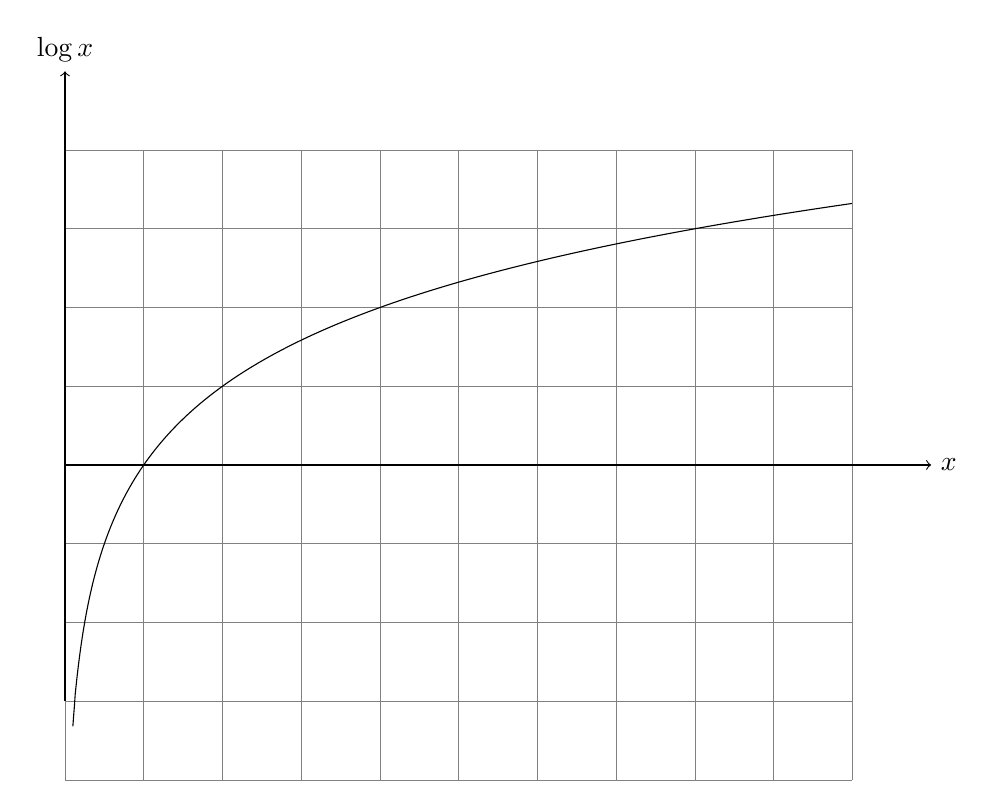
\begin{tikzpicture}
    \draw [help lines] (0,-4) grid [step=1] (10,4);
    \draw (0,0) -- (10,0);
    \draw[->] (0, 0) -- (11, 0) node[right] {$x$};
    \draw[->] (0, -3) -- (0, 5) node[above] {$\log x$};
    \draw plot [domain=0.1:10,samples=1000] (\x,{log2(\x)});
  \end{tikzpicture}
  \caption{Graph of $\log 2$}
\end{center}
\end{figure}

So we can see that rate of increment of logarithm function decreases. Rate of increment of logarithm function is given by
$\frac{1}{x}$ at any point $x$, as we will learn when we study Calculus and derivatives.

\section{Problems}
\begin{enumerate}
\item Find the value of $x$, where $\log_{\sqrt{8}} x = \frac{10}{3}$.
\item Prove that $\log_ba.\log_cb.\log_ac = 1$.
\item Prove that $\log_3\log_2\log_{\sqrt{5}}625 = 1$.
\item If $a^2 + b^2 = 23ab$, then prove that $\log\tfrac{a + b}{5} = \frac{1}{2}(\log a + \log b)$.
\item Prove that $7\log\frac{16}{15} + 5\log\frac{25}{24} + 3\log\frac{81}{80} = \log 2$.
\item Find the value of $\log\tan1^\circ + \log\tan2^\circ + \ldots + \log\tan89^\circ$.
\item Evaluate $\log_9\tan\frac{\pi}{6}$.
\item Evaluate $\frac{\log_{a^2}b}{\log_{\sqrt{a}}b^2}$.
\item Evaluate $\log_{\sqrt{5}}.008$.
\item Evaluate $\log_{2\sqrt{3}}144$.
\item Prove that $\log_3\log_2\log_{\sqrt{3}}81 = 1$.
\item Prove that $\log_ax\log_by = \log_bx\log_ay$.
\item Prove that $\log_2\log_2\log_216 = 1$.
\item Prove that $\log_ax = \log_bx\log_cb\ldots\log_nm\log_an$.
\item Prove that $a^x = 10^x\log_{10}a$.
\item If $a^2 + b^2 = 7ab$, prove that $\log\left\{\tfrac{1}{3}(a + b)\right\} = \frac{1}{2}(\log a + \log b)$.
\item Prove that $\frac{\log a\log_ab}{\log b\log_ab} = -\log_ab$.
\item Prove that $\log(1 + 2 + 3) = \log 1 + \log 2 + \log 3$.
\item Prove that $2\log(1 + 2 + 4 + 7 + 14) = \log 1 + \log 2 + \log 4 + \log 7 + \log 14$.
\item Prove that $\log 2 + 16\log\frac{16}{15} + 12\log\frac{25}{24} + 7\log\frac{81}{80} = 1$.
\item Simplify $\frac{\log_911}{\log_513}\div\frac{\log_311}{\log_{\sqrt{5}}}13$.
\item Simplify $3^{\sqrt{\log_32}} - 2^{\sqrt{\log_23}}$.
\item Find the least integer $n$ such that $7^n > 10^5$, given that $\log_{10}343 = 2.5353$.
\item If $a, b, c$ are in G.P., prove that $\log_ax, \log_bx, \log_cx$ are in H.P.
\item Prove that $\log\sin8x = 3\log2 + \log\sin x + \log\cos x + \log\cos2x + \log\cos4x$.
\item If $x = \log_{2a}a, y = \log_{3a}2a$ and $z = \log_{4a}3a$ then prove that $xyz + 1 = 2yz$.
\item If $a$ and $b$ are the lengths of the sides and $c$ be the length of the hypotenuse of a right-angle triangle and $c - b \neq
  1$ and $c + b\neq 1$, prove that $\log_{c + b}a + \log_{c - b}a = 2\log_{c + b}a\log_{c - b}a$.
\item If $\frac{\log x}{y - z} = \frac{\log y}{z - x} = \frac{\log z}{x - y}$, then prove that $x^xy^yz^z = 1$.
\item If $\frac{yz\log(yz)}{y + z} = \frac{zx\log(zx)}{z + x} = \frac{xy\log(xy)}{x + y}$, prove that $x^2 = y^y = z^2$.
\item Prove that $(yz)^{\log y - \log z}(zx)^{\log z - \log x}(xy)^{\log x - \log y} = 1$.
\item Prove that $\frac{1}{\log_2N} + \frac{1}{\log_3N} + \ldots + \frac{1}{\log_{1988}N} = \frac{1}{\log_{1988!}N}$.
\item If $0<x<1$, prove that $\log(1 + x) + \log(1 + x^2) + \log(1 + x^4) + \ldots$ to $\infty = -\log(1 - x)$.
\item Find the sum of the series $\frac{1}{\log_2a} + \frac{1}{\log_4a} + \ldots$ up to $n$ terms.
\item If $\log_410 = x, \log_220 = y$ and $\log_58 = z$, prove that $\frac{1}{x + 1} + \frac{1}{y + 1} + \frac{1}{z + 1} = 1$.
\item If $x = \log_abc, y = \log_bca, z = \log_cab$, prove that $\frac{1}{x + 1} + \frac{1}{y + 1} + \frac{1}{z + 1} = 1$.
\item Prove that $\frac{1}{1 + \log_ba + \log_bc} + \frac{1}{1 + \log_ca + \log_cb} + \frac{1}{1 + \log_ab + \log_ac} = 1$.
\item Prove that $x^{\log y - \log z}y^{\log z - \log x}z^{\log x - \log y} = 1$.
\item If $\frac{\log a}{y - z} = \frac{\log b}{z - x} = \frac{\log c}{x - y}$, prove that $a^xb^yc^z = 1$.
\item If $\frac{x(y + z - x)}{\log x} = \frac{y(z + x - y)}{\log y} = \frac{z(x + y - z)}{x - y}$, prove that $y^zz^y = z^xx^z =
  x^yy^x$.
\item If $\frac{\log a}{b - c} = \frac{\log b}{c - a} = \frac{\log c}{a - b},$ prove that $a^{b + c}b^{c + a}c^{a + b} = 1$.
\item If $\frac{\log x}{q - r} = \frac{\log y}{r - p} = \frac{\log z}{p - q}$, prove that $x^{q + r}y^{r + p}z^{p + q} =
  x^py^qz^r$.
\item If $y = a^{\frac{1}{1 - \log _ax}}$ and $z = a^{\frac{1}{1 - \log_ay}}$, prove that $x = a^{\frac{1}{1 - \log_az}}$.
\item Let $f(x) = \frac{1}{1 - \log_ex}$, $f(y) = e^{f(z)}$ and $z = e^{f(x)}$, prove that $x = e^{f(y)}$.
\item Show that $\frac{1}{\log_2n} + \frac{1}{\log_3n} + \frac{1}{\log_4n} + \ldots + \frac{1}{\log_{43}n} =
  \frac{1}{\log_{43!}n}$.
\item Show that $2(\log a + \log a^2 + \log a^3 + \ldots + \log a^n) = n(n + 1)\log a$.
\item Find the number of digits in $12^{12}$, without actual computation. [Given $\log 2 = 0.301$ and $\log 3 = 0.477$]
\item How many positive integers have a characteristics of $2$ when base is $3$.
\item Prove that $\log_ax\log_by = \log_bx\log_ay$.
\item If $a, b, c$ are in G.P., prove that $\log_ax, \log_bx, \log_cx$ are in H.P.
\item How many zeros are there between the decimal point and first significant digit in $0.0504^{10}?$ Given $\log 2 = 0.301, \log
  3 = 0.477, \log 7 = 0.845$.
\item Find the number of digits in $72^{15}$ without actual computation. Given $\log 2 = 0.301$ and $\log  3 = 0.477$.
\item How many positive integers have characteristics $2$ when base is $5$?
\item If $\log 2 = 0.301$ and $\log 3 =0.477$, find the number of digits in $3^{15}\times 2^{10}$.
\item If $\log 2 = 0.301$ and $\log 3 =0.477$, find the number of digits in $6^{20}$.
\item If $\log 2 = 0.301$ and $\log 3 =0.477$, find the number of digits in $5^{25}$.
\item Solve $\log_a[1 + \log_b\{1 + \log_c(1 + \log_px)\}] = 0$.
\item Solve $\log_7\log_5(\sqrt{x + 5} + \sqrt{x}) = 0$.
\end{enumerate}

\noindent Solve the following equations:

\begin{enumerate}[resume]
\item $\log_2x + \log_4(x + 2) = 2$.
\item $\log_{x + 2}x + \log_x(x + 2) = \frac{5}{2}$.
\item $\log(x + 1) = 2\log x$.
\item $2\log_xa + \log_{ax}a + 3\log_{a^2x}a = 0.$ Given $a > 0$.
\item $x + \log_{10}(1 + 2^x) = x\log_{10}5 + \log_{10}6$.
\item $x^{\tfrac{3}{4}(\log_2x)^2 + \log_x{2 - \tfrac{5}{4}}} = \sqrt{2}$.
\item $(x^2 + 6)^{\log_3x} = (5x)^{\log_3x}$.
\item $(3 + 2\sqrt{2})^{x^2 - 6x + 9} + (3 - 2\sqrt{2})^{x^2 - 6x + 9} = 6$.
\item $\log_8\left(\tfrac{8}{x^2}\right)\div(\log_8x)^2 = 3$.
\item $\sqrt{\log_2(x)^4} + 4\log_4\sqrt{\tfrac{2}{x}} = 2$.
\item $2\log_{10}x - \log_x0.01 = 5$.
\item $\log_{\sin x}2\log_{\cos x}2 + \log_{\sin x}2 + \log_{\cos x}2 = 0$.
\item $2^{x + 3} + 2^{x+2} + 2^{x + 1} = 7^x + 7^{x - 1}$.
\item $\log_{\sqrt{2}\sin x}(1 + \cos x) = 2$.
\item $\log_{10}[198 + \sqrt{x^3 - x^2 - 12x + 36}] = 2$.
\item If $\log 2 = 0.30103$ and $\log 3 = 0.47712,$ solve the equation $2^x3^{2x} - 100 = 0$.
\item $\log_x3\log_{\frac{x}{3}}3 + \log_{\frac{x}{81}}3 = 0$.
\item $\log_{(2x + 3)}(6x^2 + 23x + 21) = 4 - \log_{(3x + 7)}(4x^2 + 12x + 9)$.
\item $\log_2(x^2 - 1) = \log_{\frac{1}{2}}(x - 1)$.
\item $\log_5\left(5^{\tfrac{1}{x} + 125}\right) = \log_56 + 1 + \frac{1}{2x}$.
\item $\log_{100}|x + y| = \frac{1}{2}$ and $\log_{10}y - \log_{10}|x| = \log_{100}4$.
\item $2\log_2\log_2x + \log_{\tfrac{1}{2}}\log_2(2\sqrt{2}x) = 1$.
\item $\log_{\tfrac{3}{4}}\log_8(x^2 + 7) + \log_{\tfrac{1}{2}}\log_{\tfrac{1}{4}}(x^2 + 7)^{-1} = 2$.
\item $\log_{10}x + \log_{10}x^{\tfrac{1}{2}} + \log_{10}x^{\tfrac{1}{4}} + \ldots$ to $\infty = y$ and $\frac{1 + 3 + 5 + \ldots +
  (2y - 1)}{4 + 7 + 10 + \ldots + (3y + 1)} = \frac{20}{7\log_{10}x}$.
\item $18^{4x - 3} = (54\sqrt{2})^{3x - 4}$.
\item $4^{\log_93} + 9^{\log_24} = 10^{\log_x83}$.
\item $3^{4\log_9(x + 1)} = 2^{2\log_2(x + 3)}$.
\item $\frac{6}{5}a^{\log_ax\log_{10}a\log_a5} - 3^{\log_{10}\tfrac{x}{10}} = 9^{\log_{100}x + \log_42}$.
\item $2^{3x + \frac{1}{2}} + 2^{x + \frac{1}{2}} = 2^{\log_26}$.
\item $(5 + 2\sqrt{6})^{x^2 - 3} + (5 - 2\sqrt{6})^{x^2 - 3} = 10$.
\item For $x> 1$, show that $2\log_{10x}x - \log_x{.01}\geq 4$.
\item Show that $|\log_b a + \log_ab| > 2$.
\item Solve $\log_{0.3}(x^2 + 8) > log_{0.3}9x$.
\item Solve $\log_{x - 2}(2x - 3) > \log_{x - 2}(24 - 6x)$.
\item Find the interval in which $x$ will lie if $\log_{0.3}(x - 1) < \log_{0.09}(x - 1)$.
\item Solve $\log_{\tfrac{1}{2}}x \geq \log_{\tfrac{1}{3}}x$.
\item Solve $\log_{\tfrac{1}{3}}\log_4(x^2 - 5) > 0$.
\item Solve $\log(x^2 -2x -2)\leq 0$.
\item Solve $\log_2^2(x-1)^2 - \log_{0.5}(x - 1) > 5$.
\item Prove that $\log_217\log_{\tfrac{1}{5}}2\log_3\tfrac{1}{5} > 2$.
\item Show that $\log_{20}3$ lies between $\frac{1}{2}$ and $\frac{1}{3}$.
\item Show that $\log_{10}2$ lies between $\frac{1}{4}$ and $\frac{1}{3}$.
\item Solve $\log_{0.1}(4x^2 - 1) > \log_{0.1}3x$.
\item Solve $\log_2(x^2 - 24) > \log_25x$.
\item Show that $\frac{1}{\log_3\pi} + \frac{1}{\log_4\pi} > 2$.
\item Without actual computation find greater among $(0.01)^{\tfrac{1}{3}}$ and $(0.001)^{\tfrac{1}{5}}$.
\item Without actual computation find greater among $\log_23$ and $\log_311$.
\item Solve $\log_3(x^2 + 10) > \log_37x$.
\item Solve $x^{\log_{10}x} > 10$.
\item Solve $\log_2x\log_{2x}2log_24x > 1$.
\item Solve $\log_2x\log_32x + \log_3x\log_24x > 0$.
\item Find the value of $\log_{12}60$ if $\log_630 = a$ and $\log_{15}24 = b$.
\item If $\log_ax, \log_bx$ and $\log_cx$ are in A.P. and $x\neq 1$, prove that $c^2 = (ac)^{\log_ab}$.
\item If $a = \log_{\tfrac{1}{2}}\sqrt{0.125}$ and $b = \log_3\left(\frac{1}{\sqrt{24} - \sqrt{17}}\right)$ then find whether $a >0,
  b> 0$.
\item Which one is greater among $\cos(\log_e\theta)$ and $\log_e(\cos\theta)$ if $e^{-\tfrac{\pi}{2}} < \theta < \frac{\pi}{2}$.
\item If $\log_2x + \log_2y \geq 6$, prove that $x + y\geq 16$.
\item If $a,b,c$ eb three distinct positive numbers, each different from $1$ such that $\log_ba\log_ca - \log_qaa + \log_ab\log_cb
  - \log_bb + \log_ac\log_bc - \log_cc = 0$.
\item If $y = 10^{\tfrac{1}{1 - \log x}}$ and $z = 10^{\tfrac{1}{1 - \log y}}$, prove that $x = 10^{\tfrac{1}{1 - \log z}}$.
\item If $n$ is a natural number such that $n = p_1^{a_1}p_2^{a_2}p_3^{a_3}\ldots p_k^{a_k}$ and $p_1, p_2, p_3, \ldots, p_k$ are
  distinct primes, then show that $\log n\geq k\log 2$.
\item The numbers $3, 3\log_yx, 3\log_zy, 7\log_xz$ form and A.P. then prove that $x^{18} = y^{21} = z^{28}$.
\item Prove that $\log_418$ is an irrational number.
\item If $x, y, z> 1$ are in G.P. then prove that $\frac{1}{1+ \ln x}, \frac{1}{1 + \ln y}, \frac{1}{1 + \ln z}$ are in H.P.
\item Find the value of $\log_{30}8$, if $\log_{30}3 = a$ and $\log_{30}5 = b$.
\item Find the value of $\log_{54}168$, if $\log_712 = a$ and $\log_{12}24 = b$.
\item If $a\neq 0$ and $\log_x(a^2 + 1) < 0$ then find the interval in which $x$ lies.
\item If $\log_{12}18 - a$ and $\log_{24}54=b$, prove that $ab + 5(a - b) = 1$.
\item If $a,b,c$ are in G.P., show that $\log_ax, \log_bx, \log_cx$ are in H.P.
\item If $a, a_1, a_2, \ldots, a_n$ are in G.P. and $b, b_1, b_2, \ldots, b_n$ in A.P. with positive terms and also the common
  difference of A.P. and common rations of G.P. are positive, show that there exists a system of logarithm for which $\log a_n -
  b_n = \log a - b$ for any $n$. Find the base of this system.
\item If $\log_32, \log_3(2^x - 5)$ and $\log_3\left(2^x - \frac{7}{2}\right)$ are in A.P., find the value of $x$.
\item Prove that $\log_27$ is an irraational number.
\item If $\log_{0.5}(x - 2) < \log_{0.25}(x - 2)$, then find the interval in which $x$ lies.
\end{enumerate}

\chapter{Progressions}
There are three different progressions: arithmetic progression, geometric progression and harmonic progression. We start this
chapter with arithmetic progression or A.P.

\section{Arithmetic Progressions}
Consider sequences like $1, 2, 3, 4, \ldots$ or $-1, -2, -3, -4, \ldots$ or $1, 3, 5, 7, \ldots$ or $a, a + d, a + 2d, \ldots$

These sequences increase or decrease with a common difference. When quantities increase or decrease with a common difference they
are said to be in \textit{Arithmetic Progression}. The \textit{common difference} can be found by subtracting any term of the
series that follows it. For example for the first series it is $1$ and for the last it is $d$.

Consider the series $a, a + d, a + 2d, a + 3d, \ldots$

Simple observation tells us that $1$st term is $a$, $2$nd term is $a + d$, the $3$rd term is $a + 2d$ and hence the $n$th term will
be $a + (n - 1)d$. These terms are typically written as $t_1, t_2, t_3, \ldots, t_n$.

\subsection{$n$th Term of Arithmetic Progression}
Following above discussion, we can clearly say that the $n$th term of an arithmetic progression is given by $t_n = a + (n - 1)d$,
where $a$ is called the first term and $d$ the common difference.

\subsection{Sum of an Arithmetic Progression}
Let $S_n$ represent the sum of first $n$ terms of an arithmetic progression, then we can write.

$$S_n = a + (a + d) + (a + 2d) + \ldots + [a + (n - 2)d] + [a + (n - 1)d]$$
Writing the terms in reverse order we have
$$S_n = [a + (n - 1)s] + [a + (n - 2)d] + \ldots + (a + d) + a$$
Adding term by term, we get
$$2S_n = [2a + (n - 1)d] + [2a + (n - 1)d] + \ldots\text{~to~}n\text{~terms~}$$
$$2S_n = n[2a + (n - 1)d]\Rightarrow S_n = \frac{n}{2}[2a + (n - 1)d]$$

We also see that $S_n = \frac{n}{2}(t_1 + t_n)$

We also see that if a series is $1 + 2 + 3 + \ldots + n = \sum_{i=0}^ni = \frac{n(n + 1)}{2}$.

\subsection{Arithmetic Mean}
When three quantities are in arithmetic progression the quantity in the middle is known to be arithmetic mean of the other two. For
example, if $a, b, c$ are in A.P., then $b$ is said to be arithmetic mean of $a$ and $c$. In general, it is written $b = \frac{a +
  c}{2}$. This can be examined further. Let $b = a + d$, then $c = a + 2d$. Clearly, $b = \frac{a + c}{2}$.

It is also possible to insert $n$ numbers between any two numbers such that all of them are in A.P. Consider two numbers $a$ and
$b$ in between which we want to insert $n$ numbers such that they are in A.P. Clearly, $b$ will become $n +2$th term of A.P. Let
common difference be $d$ then we can write $b = a + (n + 1)d \Rightarrow d = \frac{b - a}{n + 1}$. Now all the $n$ arithmetic means
can be deduced. Let those be $m1, m2, \ldots, m_n$ then $m_1 = a + \frac{b - a}{n + 1}, m_2 = a + \frac{2(b - a)}{n + 1}, \ldots,
m_n = a + \frac{n(b - a)}{n + 1}$.

First A.M. $= a + d = \frac{an + b}{n +1}$

Second A.M. $= a + 2d = \frac{a(n - 1) + b}{n + 1}$

$\ldots$

$n$th A.M. $= a + nd = \frac{a + nb}{n + 1}$

Suppose there are $n$ terms of an A.P., then the arithmetic mean of those $n$ terms is given by $\frac{t_1 + t_2 + \ldots +
  t_n}{n}$.

\subsection{Deducing Number of Terms}
We know that $S_n = \frac{n}{2}[2a + (n - 1)d]$. Say $S_n, a$ and $d$ are known and we have to evaluate $n$. This being a quadratic
equaion will have two roots for $n$. If the results are positive and integral then there is no problem in interpreting the
results. In some cases for a negative root a suitable interpretation can be given.

\textbf{Example:} How many terms of the series $-8, -6, -4, \ldots$ must be added for the sum to be $36$?

$\frac{n}{2}[-16 + (n - 1)2] = 36\Rightarrow n^2 - 9n - 36 = 0 \Rightarrow n = 12, -3$

If we take $12$ terms of the series, we have $-8, -6, -4, -2, 0, 2, 4, 6, 8, 10, 12, 14$. The sum of these terms is $36$ and sum of
last three terms is also $36$ which is represented by $n = -3$.

\subsection{Properties of an A.P.}
\begin{enumerate}
\item If a fixed number is added to or subtracted from each item of a given A.P., then the resulting is also an A.P., and it has
  the same common difference as that of the given A.P.
\item If each term of an A.P. is multiplied or divided by a non-zero fixed constant then the resulting sequence is also an A.P. The
  common difference is multiplied or divided by the same factor.
\item If $a_1, a_2, a_3, \ldots$ and $b_1, b_2, b_3, \ldots$ are two arithmetic progressions then $a_1 + b_1, a_2 + b_2, a_3 + b_3,
  \ldots$ are also in A.P.
\item If we have to choose three unknown terms in an A.P. then it is best to choose them as $a - d, a, a + d$.
\item If we have to choose four unknown terms in an A.P. then it is best to choose them as $a - 3d, a - d, a + d, a + 3d$.
\item In an A.P., the sum of terms equidistant from the beginning and end is constant and is equal to the sum of first and last
  term.
\item Any term of an A.P., except the first, is equal to half the sum of terms which are equidistant from it:
  $$a_n = \frac{1}{2}(a_{n - k} + a_{n + k}), ~k<n,\text{~and for~} k = 1$$
  $$a_n = \frac{1}{2}(a_{n - 1} + a_{n + 1})$$
\item $t_n = S_n - S_{n - 1}, n\geq 2$
\item If $t_n = pn + q$ i.e. a linear expression in $n$ then it will form an A.P. of common difference $p = t_n - t_{n - 1}$ and
  first term $p + q$. For example, if $t_n = 3n + 4$, then it is an A.P. of common difference $3$ anda the first term as $7$.
\item If $S_n = an^2 + bn + c$ i.e. a quadratic function in $n$, then the series in an A.P. where $a = 2a,$ twice the coefficient
  of $n^2$.
\end{enumerate}

\subsection{Sum of Squares and Cubes and More}
We observe that
$$i^3 - (i - 1)^3 = 3i^3 - 3i + 1 \Rightarrow \sum_{i = 1}^n[i^3 - (i - 1)^3] = 3\sum_{i = 0}^ni^2 - \frac{3n(n + 1)}{2} + n$$
$$n^3 = 3\sum_{i = 0}^ni^2 - \frac{3n(n + 1)}{2} + n \Rightarrow 3\sum_{i=0}^ni^2 = n^3 + \frac{3n(n + 1)}{2} - n$$
$$\sum_{i=0}^ni^2 = \frac{n(n + 1)(2n + 1)}{6}$$

Following in a similar fashion, we can show that

$$\sum_{i=0}^n = \left\{\frac{n(n + 1)}{2}\right\}^2$$

More powers can be evaluated in a similar fashion.

\section{Geometric Progressions}
A succession of numbers is said to be in geometric progressions or geometric sequence if the ratio of any term and the term
preceeding it is constant throughout. This constant is called \textit{common ratio} of the G.P.

Example: $1, 2, 4, 8, 16, \ldots$

Here, $\frac{t_2}{t_1} = \frac{t_3}{t_2} = \ldots = 2$.

Also, $1, 3, 9, 27,\ldots$ are in geometric progression whose first term is $1$ and common ratio is $3$.

Also, $2, -4, 8, -16, \ldots$ are in geometric progression whose firts term is $2$ and common ratio is $-2$.

\subsection{Properties of a G.P.}
\begin{enumerate}
\item If the each term of a G.P. be multiplied by a non-zero number, then the sequence obtained is also a G.P.

  \textbf{Proof:} Let the given G.P. be $a, ar, ar^2, ar^3, \ldots$

  Let $k$ be a non-zero number, the sequence obtained by multiplying each term of the given G.P. by $k$ is $ak, ark, ar^2k, ar^3k,
  \ldots$

  Clearly, the series is in G.P. with the same common ratio as previous ratio i.e. $r$.

  Again, dividing each term of G.P. $a, ar, ar^2, a^3, \ldots$ we obtain the sequence $\frac{a}{k}, \frac{ar}{k}, \frac{ar^2}{k},
  \ldots$

  It is clear that this new sequence is also a G.P., whose common ratio is $r$.
\item The reciprocals of the terms of a G.P. are also in G.P.

  \textbf{Proof:} Let the G.P. be $a, ar, ar^2, \ldots$, the sequence whose terms are reciprocals of this G.P. is $\frac{1}{a},
  \frac{1}{ar}, \frac{1}{ar^2}, \ldots$

  It is clear that this sequence is in G.P., whose first term is $\frac{1}{a}$ and common ratio is $\frac{1}{r}$.
\end{enumerate}

\subsection{Sum of the First $n$ Terms of a G.P.}
Let $a$ be the first term and $r$ be the common ratio of a G.P. and $S_n$ be the sum of its first $n$ terms

\textbf{Case I:} When $r\neq 1$
$$S_n = a + ar + ar^2 + \ldots + ar^{n - 2} + ar^{n - 1}$$
$$rS_n = ar + ar^2 + \ldots + ar^{n - 1} + ar^n$$

Subtracting, we get $(1 - r)S_n = a - ar^n = a(1 - r^n)$

$\therefore S_n = \frac{a(1 - r^n)}{1 - r} = \frac{a(r^n - 1)}{r - 1}$

\textbf{Case II:} When $r = 1$

$S_n = a + a + \ldots + a = na$ and this G.P. is also an A.P. whose common difference is $0$.

\subsection{Sum of Infinite Terms of a G.P.}
If $|r|\geq 1$ then sum would be $\pm\infty$. However, if $|r|< 1$ then sum would be finite.

We have obtained that $S_n = \frac{a(1 - r^n)}{1 - r}$

We see that as $n$ approaches $\infty, r^n$ will approach $0$. Thus, $S_\infty = \frac{a}{1 - r}$

\subsection{Recurring Decimals}
Recurring decimals are a very interesting and nice example to demonstrate the infinite G. P. and the value can be obtained by the
formula derived in previous section. Consider a recurring decimal $\dot{7}$.

$$.\dot{7} = .777777 ... \text{to }\infty$$
$$= .7 + .07 + .007 + .0007 + \ldots$$
$$= \frac{7}{10} + \frac{7}{100} + \frac{7}{1000} + \ldots$$
$$= \frac{7}{10} + \frac{7}{10^2} + \frac{7}{10^3} + \ldots$$
$$= 7\left(\frac{1}{10} + \frac{1}{10^2} + \frac{1}{10^3} + \ldots\right)$$
$$= \frac{7}{9}$$

\subsection{Geometric Mean}
Like arithmetic means; we also have geometric means. Say two numbers $a$ and $b$ are in G.P. and $x$ is a geometric mean between
them then by definition $a, x, b$ will be in G.P. Then,
$$\frac{x}{a} = \frac{b}{x}$$
$$\Rightarrow x^2 = ab \Rightarrow x = \sqrt{ab}$$

If $G_1, G_2, \ldots, G_n$ are $n$ geometric means between two numbers $a$ and $b$, then $G_1G_2\ldots G_n = \sqrt{ab^n}$

\noindent\textbf{Proof:} $b$ is the $n + 2$nd term. Thus, $b = ar^{n + 1}$ where common ratio is $r$.

Thus, $G_1 = ar, G_2 = ar^2, \ldots, G_n = ar^n$

$G_1G_2\ldots G_n = ar^{1 + 2 + \ldots + n} = ar^{\frac{n(n + 1)}{2}}$

$= \sqrt{ab^n}$

If $a_1, a_2, \ldots, a_n$ are $n$ positive numbers in G.P. then their geometric mean is given by $G = (a_1a_2\ldots
a_n)^{\frac{1}{n}}$

Thus, first G.M. $= ar = a\left(\frac{b}{a}\right)^{1/(n + 1)}$

Second G.M. $= ar^2 = a\left(\frac{b}{a}\right)^{2/(n + 1)}$

$\ldots$

$n$th G.M. $= ar^{n} = a\left(\frac{b}{a}\right)^{n/(n + 1)}$
\subsection{Notes}
\begin{enumerate}
\item Odd number of terms in a G.P. should be taken as $\ldots\frac{a}{r^2}, \frac{a}{r}, a, ar, ar^2, \ldots$
\item Even number of terms in a G.P. should be taken as $\ldots, \frac{a}{r^5}, \frac{a}{r^3}, \frac{a}{r}, ar, ar^3, ar^5, \ldots$
\item If $a_1, a_2, \ldots, a_n$ and $b_1, b-2, \ldots, b_n$ be two G.P. of common ratios $r_1$ and $r_2$ then $a_1b_1, a_2b_2,
  a_3b_3, \ldots$ and $\frac{a_1}{b_1}, \frac{a_2}{b_2}, \frac{a_3}{b_3}, \ldots$ also form G.P., where common ratios will be
  $r_1r_2$ and $\frac{r_1}{r_2}$ respectively.
\item Let $a_1, a_2, a_3, \ldots$ be a G.P. of positive terms, then $\log a_1, \log a_2, \log a_3, \ldots$ will be an A.P. and
  vice-versa.

  Let $a$ be the first term and $r$ be the common ratio of the G.P. then $a_i = ar^{i - 1}$. Now $\log a_i = \log a + (i - 1)\log
  r$ which represents $i$th term of an A.P. with first term as $\log a$ and common difference $\log r$.

  Conversely, let us assume that $\log a_1, \log a_2, \log a_3, \ldots$ are in A.P. then $a_i = x^{a + (i - 1)d} = x^ax^{{i - 1}d}$
  where $x$ is the base of the logarithm. This shows that $a_1, a_2, a_3,\ldots$ will be in G.P., whose first term is $x^a$ and
  whos ecommon ratio is $x^d$.
\item Increasing and decreasing G.P.

  \textbf{Case I:} Let the first term $a$ be positive. Then if $r > 1$, then it is an increasing G.P. but if $0< r< 1$ then it is a
  decreasing G.P.

  \textbf{case II:} Let the first term $a$ be negative. Then if $r > 1$, then it is a decreasing G.P. but if $0 < r < 1$ then it is
  an increasing G.P.
\end{enumerate}

\subsection{Arithmetico Geometric Series}
If the termms of an A.P. are multiplied y corresponding terms of a G.P., then the new series obtained is called an
Arithmetico-Geometric series.

\textbf{Exmaple:} If the terms of the arithmetic series $2 + 5 + 8 + \ldots$ are multiplied with the corresponsing terms of the
geometric series $x + x^2 + x^3 + \ldots$ then the resulting arithmetico-geometric series is $2x + 5x^2 + 8x^3 + \ldots$

\subsection{Sum of $n$ terms of an Arithmetico-Geometric Series}
Let $a_1, a_2, \ldots, a_n$ be an A.P. and $b_1, b_2, \ldots, b_n$ be a G.P. Let $d$ be the common difference of the A.P. and $r$
be the common ratio of the G.P. Also, let $a = a_1$ and $b = b_1$, then
$$S_n = ab + (a + d)br + (a+ 2d)br^2 + \ldots + [a + (n - 1)d]br^{n - 1}$$
$$rS_n = abr + (a + d)br^2 + (a + 2d)br^3 + \ldots + [a + (n - 1)d]br^n$$
$$\Rightarrow (1 - r)S_n = ab + dbr + dbr62 + \ldots + dbr^{n - 1} - [a + (n - 1)d]br^n$$
$$= ab + \frac{dbr(1 - r^{n - 1})}{(1 - r) - [a + (n - 1)d]br^n}$$
$$S_n = \frac{ab}{1 - r} + \frac{dbr(1 - r^{n - 1})}{(1 - r)^2} - \frac{[a + (n - 1)d]br^n}{1 - r}(r\neq 1)$$

If $|r|< 1$, then $lim_{n\to \infty}r^n = 0$, therefore , sum of an infinite number of terms of an arithmetico-geometric series is
given by
$$S_\infty = \frac{ab}{1 - r} + \frac{dbr}{(1 - r)^2}$$

\section{Harmonic Progressions}
Consider an A.P. then an H.P. is formed by terms given by reciprocal of terms of the A.P. respectively. So if the terms of A.P. are
$a_1, a_2, \ldots, a_n$ then terms of H.P. are given by $\frac{1}{a_1}, \frac{1}{a_2}, \ldots, \frac{1}{a_n}$.

When we study H.P. and its properties we do that by studying the properties of the corresponding A.P.

\subsection{Harmonic Means}
Numbers $H_1, H_2, \ldots, H_n$ are said to be the $n$ H.M. between two numbers $a$ and $b$, if $a, H_1, H_2, \ldots, H_n, b$ are
in H.P. For example, $\frac{1}{2}, \frac{1}{3}, \frac{1}{4}$ are the H.M. between $1$ and $\frac{1}{5}$ because $1, \frac{1}{2},
\frac{1}{3}, \frac{1}{4}, \frac{1}{5}$ are in H.P.

Let $a$ and $b$ be the two given quantities and $H$ be the H.M. between them. Then $a, H, b$ will be in H.P.

$\therefore \frac{1}{a}, \frac{1}{H}, \frac{1}{b}$ will be in H.P.

$\frac{1}{H} - \frac{1}{a} = \frac{1}{b} - \frac{1}{H} \Rightarrow H = \frac{2ab}{a =b}$

Let $H_1, H_2, \ldots, H_n$ be the $n$ H.M. between two given quantities $a$ and $b$, and $d$ be the c.d. of the corresponding A.P.
Then $a, H_1, H_2, \ldots, H_n, b$ will be in H.P.

$\therefore \frac{1}{a}, \frac{1}{H_1}, \frac{1}{H_2}, \ldots, \frac{1}{H_n}, \frac{1}{b}$ will be in A.P.

$\frac{1}{b} = t_{n + 2} = \frac{1}{a} + (n + 1)d \Rightarrow d = \frac{a - b}{ab(n + 1)}$

$\therefore \frac{1}{H_1} = \frac{1}{a} + d \Rightarrow H_1 = \frac{ab(n + 1)}{a + nb}$

$H_2 = \frac{ab(n + 1)}{2a + (n - 1)b}$

$\ldots$

$H_n = \frac{ab(n + 1)}{an + b}$

\section{Relation between A.M., G.M. and H.M.}
Let $a$ and $b$ be two real, positive and unequal quantities and $A, G$ and $H$ be the single A.M., G.M. and H.M. between them
respectively.

Then, $A = \frac{a + b}{2}, G = \sqrt{ab}, H = \frac{2ab}{a + b}$

$AH = ab = G^2$ and thus $A, G, H$ form a G.P.

Similarly it can be probve that $A > G > H$

For equal $a$ and $b$, it can be easily verified that $A = G = H$

\section{Problems}
\begin{enumerate}
\item If $n$th term of a sequence is $2n^2 + 1,$ find the sequence. Is this seuquence in A.P.?
\item Find the first five terms of the sequence for which $t_1 = 1, t_2 = 2$ and $t_{n + 2} = t_n + t_{n + 1}$.
\item Write the sequence whose $n$th term is $3n + 5$.
\item Write the sequence whose $n$th term is $2n^2 + 3$.
\item Write the sequence whose $n$th term is $\frac{3n}{2n + 4}$.
\item Write the first three terms of sequence defined by $t_1 = 2, t_{n + 1} = \frac{2t_n + 1}{t_n + 3}$.
\item If $n$th term of a sequence is $4n^2 + 1$, find the sequence. Is this sequence an A.P.?
\item If $n$th term of a sequence is $2an + b$, where $a, b$ are constants, is this sequence an A.P.?
\item Find the 5th term of the sequence whose first three terms are $3, 3, 6$ and each term after the second is the sum of two
  preceding terms.
\item Consider the sequence defined by $t_n = an^2 + bn + c$. If $t_1 = 1, t_2 = 5$ and $t_3 = 11$ then find the value of
  $t_{10}$.
\item Show that the seuquence $9, 12, 15, 18, \ldots$ is an A.P. Find its $16^{th}$ term and the general term.
\item Show that the sequence $\log a, \log (ab), \log(ab^2), \log (ab^3), \ldots$ is an A.P. Find its $n^{th}$ term.
\item Find the sum to $n$ terms of the sequence $\langle t_n \rangle$, where $t_n = 5 -6n, n\in N$.
\item How many terms are there in the A.P. $3, 7, 11, \ldots, 407?$
\item If $a, b, c, d, e$ are in A.P. find the value of $a - 4b + 6c - 4d + e$.
\item In a certain A.P. $5$ times the $5$th term is equal to $8$ times the $8$th term, then prove that $13$th term is
  zero.
\item Find the term of the series $25, 22\frac{3}{4}, 20\frac{1}{2},18\frac{1}{4}, \ldots$ which is numerically smallest positive
  number.
\item A person was appointed in the pay scale of Rs. $700 - 40 - 1500$. Find in how many years he will reach the maximum of the
  scale.
\item Find the A.P. whose $7$th and $13$th terms are respectively $34$ and $64$.
\item Is $55$ a term of the sequence $1, 3, 5, 7, \ldots$? If yes, find which term it is.
\item Find the first negative term of the sequence $2000, 1995, 1990, \ldots$
\item How many terms are identical in two arithmetic progressions $2, 4, 6, 8, \ldots$ up to $100$ terms and $3, 6, 9, \ldots$ up
  to $80$ terms.
\item Find the number of all positive integers of $3$ digits which are divisible by $5$.
\item Is $105$ a term of the arithmetic progression $4, 9, 14, \ldots?$
\item Find the first negative term of the sequence $999, 995, 991, \ldots$.
\item Each of the series $3 + 5 + 7 + \ldots$ and $4 + 7 + 10 + \ldots$ is continued to $100$ term. Find how many terms are
  identical?
\item If $m$ times the $m$th term of an A.P. is equal to $n$ times the $n$th term, find its $(m + n)$th term.
\item If $a, b, c$ be the $p$th, $q$th and $r$th terms respectively of an A.P., prove that $a(q - r) + b(r - p) + c(p - q) =
  0$.
\item Find the number of integers between $100$ and $1000$ that are divisible by $7$ and not divisible by $7$.
\item If $a, b, c$ be the $p$th, $q$th and $r$th terms respectively of an A.P., prove that $(a - b)r + (b - c)p + (c - a)q =
  0$.
\item The sum of three numbers in A.P. is $27$ and the sum of their squares is $293.$ Find the numbers.
\item The sum of four integers in A.P. is $24$ and their product is $945.$ Find the numbers.
\item If the $p$th term of an A.P. is $q$ and the $q$th term is $p$, find the first term and common difference. Also, show that $(p
  + q)$th term is zero.
\item For an A.P. show that $t_m + t_{2n + m} = 2t_{m + n}$.
\item Divide $15$ into three parts which are in A.P. and the sum of their squares is $83$.
\item Three numbers are in A.P. Their sum is $27$ and the sum of their squares is $275$. Find the numbers.
\item The sum of three numbers in A.P. is $12$ and the sum of their cubes is $408$. Find the numbers.
\item Divide $20$ into four parts which are in A.P. such that the product of first and fourth is to product of second and third is
  $2:3$.
\item The sum of three numbers in A.P. is $-3$ and their product is $8$. Find the numbers.
\item Divide $32$ into four parts which are in A.P. such that the ratio of product of extremes to the product of means is $7:15$.
\item If $(b + c - a)/a, (c + a - b)/b, (a + b - c)/c$ are in A.P. then prove that $1/a, 1/b, 1/c$ are also in A.P.
\item If $a, b, c \in R+$ form an A.P., then prove that $a + 1/bc, b + 1/ca, c + 1/ab$ are also in A.P.
\item If $a, b, c$ are in A. P., then prove that $a^2(b + c), b^2(c + a), c^2(a + b)$ are also in A.P.
\item If $a, b, c$ are in A.P., then prove that $\frac{1}{\sqrt{b} + \sqrt{c}}, \frac{1}{\sqrt{c} + \sqrt{a}}, \frac{1}{\sqrt{a} +
  \sqrt{b}}$ are also in A.P.
\item If $a, b, c$ are in A.P., then prove that $a\left(\frac{1}{b} + \frac{1}{c}\right), b\left(\frac{1}{c} + \frac{1}{a}\right),
  c\left(\frac{1}{a} + \frac{1}{b}\right)$ are also in A.P.
\item If $(b - c)^2, (c - a)^2, (a - b)^2$ are in A.P. then prove that $\frac{1}{b - c}, \frac{1}{c - a}, \frac{1}{a - b}$ are also
  in A.P.
\item If $a, b, c$ are in A.P. then prove that $b + c, c + a, a + b$ are also in A.P.
\item If $a^2, b^2, c^2$ are in A.P. then prove that $\frac{1}{b+c}, \frac{1}{c+a}, \frac{1}{a + b}$ are in A.P.
\item If $a, b, c$ are in A.P., show that $2(a - b) = a - c = 2(b - c)$.
\item If $a, b , c$ are in A.P., then prove that $(a - c)^2 = 4(b^2 - ac)$.
\item In an A.P. if $S_1 = t_1 + t_2 + \ldots + t_n$ ($n$ odd), $S_2 = t_2 + t_4 + \ldots + t_{n - 1},$ then find the value of
  $S_1/S_2$ in terms of $n$.
\item Find the degree of the polynomial $(1 + x)(1 + x^6)(1 + x^{11})\ldots (1+ x^{101})$.
\item Prove that a sequence is an A.P. if the sum of its terms is of the form $An^2 + Bn,$ where $A, B$ are constants.
\item If the sequence $a_1, a_2, \ldots, a_n$ form an A.P., then prove that $a_1^2 - a_2^2 + a_3^2 - a_4^2 + \ldots + a_{2n - 1}^2
  - a_{2n}^2 = \frac{n}{2n - 1}(a_1^2 - a_{2n}^2)$.
\item Find the sum of first $24$ terms of the A.P. $a_1, a_2, a_3, \ldots, a_{24},$ if it is known that $a_1 + a_5 + a_{10} +
  a_{15} + a_{20} + a_{24} = 225$
\item If the arithmetic progression whose common difference is non-zero, the sum of first $3n$ terms is equal to next $n$
  terms. Then, find the ratio of sum of first $2n$ terms to the sum of next $2n$ terms.
\item If the sum of $n$ terms of a series be $5n^2 + 3n,$ find its $n$th term. Are the terms of this series in A.P.?
\item Find the sum of the series $(a + b)^2 + (a^2 + b^2) + (a - b)^2 + \ldots$ to $n$ terms.
\item Find $1 - 3 + 5 - 7 + 9 - 11 + \ldots$ to $n$ terms.
\item The interior angles of a polygon are in A.P. The smallest angle is $120$\textdegree and the commnon difference is
  $5$\textdegree. Find the number of sides of the polygon.
\item $25$ trees are planted in a straight line at intervals of $5$ meters. To water them the gardener must bring water for each
  tree separately from a well $10$ meters from the first tree. How far he will have to travel to water all the trees beginning with
  the first if he starts from the well.
\item If $a$ be the first term of an A.P. and the sum of its first $p$ terms is equal to zero, show that the sum of the next $q$
  terms is $-\frac{a(p + q)}{p - 1}q$.
\item The sum of the first $p$ terms of an A.P. is equal to the sum of its first $q$ terms, prove that the sum of its first $(p +
  q)$ terms is zero.
\item Prove that the sum of latter half of $2n$ terms of a series in A.P. is equal to the one third of the sum of first $3n$ terms.
\item If $S_1, S_2, S_3, \ldots, S_p$ be the sum of $n$ terms of arithmetic progressions whose first terms are respectively $1, 2,
  3, \ldots$ and common differences are $1, 2, 3, \ldots$ prove that $$S_1 + S_2 + S_3 + \ldots + S_p = \frac{np}{4}(n+1)(p+1)$$
\item If $a,b$ and $c$ be the sum of $p, q$ and $r$ terms rspectively of an A.P., prove that $$\frac{a}{p}(q - r) + \frac{b}{q}(r -
  p) + \frac{c}{r}(p - q) = 0$$
\item If the sum of $m$ terms of an A.P. is equal to half the sum of $(m + n)$ terms and is also equal to half the sum of $(m + p)$
  terms, prove that $(m + n)\left(\frac{1}{m} - \frac{1}{p}\right) = (m + p)\left(\frac{1}{m} - \frac{1}{n}\right)$.
\item If there are $(2n + 1)$ terms in an A.P., then prove that the ratio of sum of odd terms and the sum of even terms is $n + 1:
  n$.
\item The sum of $n$ terms of two series in A.P. are in the ration $(3n - 13): (5n + 21)$. Find the ratio of their $24$th terms.
\item If the $m$th term of an A.P. is $\frac{1}{n}$ and $n$th term of an A.P. is $\frac{1}{m}$ then prove that the sum to $mn$
  terms is $\frac{mn + 1}{2}$.
\item If the sum of $m$ terms of an A.P.is $n$ and the sum of its $n$ terms is $m$, show that sum of $(m + n)$ terms is $-(m + n)$.
\item If $S$ be the sum of $2n + 1$ terms of an A.P., and $S_1$ that of alternate terms beginning with the first, then show that
  $\frac{S}{S_1} = \frac{2n + 1}{n + 1}$
\item If $a, b, c$ be the $1$st, $3$rd, $n$th terms respectively of an A.P., prove that the sum of $n$ terms is $\frac{c + a}{2} +
  \frac{c^2 - a^2}{b - a}$.
\item The sum of $n$ terms of two series in A.P. are in ratio $(3n + 8):(7n + 15)$. Find the ratio of their $12$th terms.
\item If the ratio of the sum of $m$ terms and $n$ terms of an A.P. is $m^2:n^2,$ prove that the ratio of its $m$th and $n$th term
  wil be $(2m - 1):(2n -1)$.
\item How many terms are in the G.P. $5, 20, 80, ..., 5120$?
\item How many terms are in the G.P. $0.03, 0.06, 0.12, \ldots, 3.84$?
\item A boy agrees to work at the rate of one rupee the first day, two rupee the second day, four rupees the third day, eight
  rupees the fourth day and so on. How much would he get on $20th$ day?
\item The population of a city in January $1987$ was $20,000$. It increased at the rate of $2\%$ per annum. Find the population of
  the city in January $1997$.
\item The sum of $n$ terms of a sequence is $2^n - 1,$ find its $n$th term. Is the sequence in G.P.?
\item If the fifth term of a G.P. is $81$ and second term is $24$. Find the G.P.
\item The seventh term of a G.P. is $8$ times the fourth term. Find the G.P. when its $5$th term is $48$.
\item If the $5$th and $8$th terms of a G.P. be $48$ and $384$ respectively, find the G.P
\item If the $6$th and $10$th terms of a G.P. are $\frac{1}{16}$ and $\frac{1}{256}$ respectively, find the G.P.
\item If the $p$th, $q$th and $r$th terms of a G.P. be $a, b, c (a, b, c >0)$, then prove that $(q - r)\log a + (r - p)\log b + (p
  - q)\log c = 0$.
\item If the $(p + q)$th term of a G.P. is $a$ and the $(p - q)$th term is $b$, show that its $p$th term is $\sqrt{ab}$.
\item If the $p$th, $q$th and $r$th terms of a G.P. be $x, y$ and $z$ respectively, prove that $x^{q - r}.y^{r - p}.z^{p - q} = 1$.
\item The first term of a G.P. is $1$. The sum of third and fifth terms is $90$. Find the common ratio of G.P.
\item Fifth term of a G.P. is $2$. Find the product of its first nine terms.
\item The fourth, seventh and last term of a G.P. are $10, 80$ and $2560$ respectively. Find the first term and number of terms in
  the G.P.
\item Three numbers are in G.P. If we double the middle term they form an A.P. Find the common ratio of the G.P.
\item If $p, q$ and $r$ are in A.P. show that $p$th, $q$th and $r$th term of a G.P. are in G.P.
\item If $a, b, c$ and $d$ are in G.P., show that $(ab + bc + cd)^2 = (a^2 + b^2 + c^2)(b^2 + c^2 + d^2)$.
\item Three non-zero numbers $a, b$ and $c$ are in A.P. Increasing $a$ by 1 or increading $c$ by 2,the numbers are in G.P. Then
  find $b$.
\item Three numbers are in G.P. whose sum is $70$. If the extremes be each multiplied by $4$ and the mean by $5$, they will be in
  A.P. Find the numbers.
\item If the product of three numbers in G.P. be $216$ and their sum is $19$, find the numbers.
\item A number consists of three digits in G.P. The sum of the right hand and left hand digits exceed twice the middle digit by $1$
  and the sum of left hand and middle digit is two-third of the sum of the middle and right hand digits. Find the number.
\item In a set of four numbers, the first three are in G.P. and the last three are in A.P. with a common difference of $6$. If the
  first number is same as fourth, find the four numbers.
\item The sum of three numbers in G.P. is $21$ and the sum of their squares is $189$. Find the numbers.
\item The prodduct of three consecutive terms of a G.P. is $-64$ and the first term is four times the third. Find the terms.
\item Three numbers whose sum is $15$ are in A.P. If $1, 4, 19$ be added to them respectively the resulting numbers are in
  G.P. Find the numbers.
\item From three numbers in G.P. other three numbers in G.P. are subtracted. Resulting numbers are found to be in G.P. again. Prove
  that the three sequences have the same common ratio.
\item If $a, b, c, d$ are in G.P., show that $(b - c)^2 + (c - a)^2 + (d - b)^2 = (a - d)^2$.
\item If $a,b,c,d$ are in G. P., then show that $(a^2 + b^2 + c^2)(b^2 + c^2 + d^2) = (ad + bc + cd)^2$.
\item If $a^x = b^y = c^z$ where $x, y, z$ are in G.P., show that $\log_ba = \log_cb$.
\item If the continued product of three numbers in a G.P. is $216$ and the sum of their products in pairs is $156$, find the
  numbers.
\item If $a, b, c, d$ are in G.P., show that $(a + b)^2, (b + c)^2, (c + d)^2$ are in G.P.
\item If $a, b, c, d$ are in G.P., show that $(a - b)^2, (b - c)^2, (c - d)^2$ are in G.P.
\item If $a, b, c, d$ are in G.P., show that $a^2 + b^2 + c^2, ab + bc + cd, b^2 + c^2 + d^2$ are in G.P.
\item If $a, b, c, d$ are in G.P., show that $\frac{1}{(a + b)^2}, \frac{1}{(b + c)^2}, \frac{1}{(c + d)^2}$ are in G.P.
\item If $a, b, c, d$ are in G.P., show that $a(b - c)^3 = d(a - b)^3$.
\item If $a, b, c, d$ are in G.P., show that $(a + b + c + d)^2 = (a + b)^2 + (c + d)^2 + 2(b + c)^2$.
\item If $a, b, c$ are in G.P., show that $a^2b^2c^2\left(\frac{1}{a^3} + \frac{1}{b^3} + \frac{1}{c^3}\right) = a^3 + b^3 + c^3$.
\item If $a, b, c$ are in G.P., show that $(a^2 - b^2)(b^2 + c^2) = (b^2 - c^2)(a^2 + b^2)$.
\item If $a, b, c$ are in G.P., show that $\log a, \log b, \log c$ are in A.P.
\item Find $1 + \frac{1}{2} + \frac{1}{4} + \frac{1}{8} + \ldots$ to $n$ terms.
\item Find $1 + 2 + 4 + 8 + \ldots$ to $12$ terms.
\item Find $1 - 3 + 9 - 27 + \ldots$ to $9$ terms.
\item Find $1 + \frac{1}{3} + \frac{1}{9} + \frac{1}{27} \ldots$ to $n$ terms.
\item Find the sum of $n$ terms of the series $(a + b) + (a^2 + 2b) + (a^3 + 3b) + \ldots$ to $n$ terms.
\item A man agrees to work at the rate of one dollar the first day, two dollars the second day, four dollars the third day, eight
  dollars the fourth day and so on. How much would he get at the end of $120$ days.
\item Find the sum to $n$ terms of the series $8 + 88 + 888 + \ldots$.
\item  Find the sum to $n$ terms of the series $6 + 66 + 666 + \ldots$.
\item Find the sum to $n$ terms of the series $4 + 44 + 444 + \ldots$.
\item Find the sum to $n$ terms of the series $.5 + .55 + .555 + \ldots$.
\item Find $1 - \frac{1}{2} + \frac{1}{4} - \frac{1}{8}$ to $n$ terms.
\item If you had a choice of a salary of a salary of $\$ 1000$ a day for a month of $31$days or $\$ 1$ for the first day, doubling
  every day which choice would you make?
\item How many terms of the series $1 + 3 + 3^2 + 3^3 + \ldots$ must be taken to make $3280$?
\item Find the least value of $n$ for which $1 + 3 + 3^2 + \ldots + 3^{n - 1} > 1000$.
\item Find $1 + \frac{1}{2} + \frac{1}{4} + \frac{1}{8}$ to $\infty$.
\item A person starts collecting \$ 1 first day, \$ 3 second day, \$ 9 third day and so on. What will be his collection in $20$
  days.
\item Find the sum of $\left(x^2 + \frac{1}{x^2} + 2\right) + \left(x^4 + \frac{1}{x^4} + 5\right) + \left(x^6 + \frac{1}{x^6} +
  8\right) + \ldots$ to $n$ terms.
\item How many terms of the series $1 + 2 + 2^2 + \ldots$ must be taken to make $511?$
\item Find the least value of $n$ such that $1 + 2 + 2^2 + \ldots + 2^{n - 1} \geq 300$.
\item Determine the no. of terms of a G.P. if $a_1 = 3, a_n = 96$ and $S_n = 189$.
\item Prove that $a^n - b^n$ is divisible by $a - b$ for any $n \in N$.
\item Prove that $a^n + b^n$ is divisible by $a + b$ for any $n \in N$.
\item Express $0.4\dot{2}\dot{3}$ as a rational number.
\item Find $\frac{1}{5} + \frac{1}{7} + \frac{1}{5^2} + \frac{1}{7^2}$ to $\infty$.
\item Prove that the sum of $n$ terms of the series $11 + 103 + 1005+ \ldots$ is $\frac{10}{9}(10^n - 1) + n^2$.
\item Find the sum to $n$ terms of the series $\left(x + \frac{1}{x}\right)^2 + \left(x^2 + \frac{1}{x^2}\right)^2 + \left(x^3 +
  \frac{1}{x^3}\right)^2 + \ldots$.
\item If $S$ be the sum, $P$ be the product and $R$ the sum of reciprocals of $n$ terms in G.P., prove that $P^2 =
  \left(\frac{S}{R}\right)^n$.
\item Find $1 + \frac{x}{1 + x} + \frac{x^2}{(1 + x)^2} + \ldots$ to $\infty$ if $x > 0$.
\item Prove that in an infinite G.P. whose common ratio is $r$ is numerically less than one, the ratio of any term to the
  sum of all the succeediing terms is $\frac{1 - r}{r}$.
\item If $S_1, S_2, S_3, \ldots, S_p$ are the sum of infinite geometric series whose first terms are $1, 2, 3, \ldots, p$
  and whose common ratios are $\frac{1}{2}, \frac{1}{3}, \frac{1}{4}, \ldots, \frac{1}{p + 1}$ respectively, prove that $S_1 + S_2
  + S_3 + \ldots + S_p = p(p + 3)/2$.
\item If $x = 1 + a + a^2 + a^3 + \ldots~\text{to}~\infty$ and $y = 1 + b + b^2 + b^3 + \ldots~\text{to}~\infty,$ show
  that $1 + ab + a^2b^2 + a^3b^3 + \ldots~\text{to}~\infty = \frac{xy}{x + y - 1},$ where $0<a< 1$ and $0<b<1$.
\item Find the sum to infinity for the series $1 + (1 + a)r + (1 + a + a^2)r^2 + \ldots,$ where $0<a<1$ and $0<r<1$.
\item After striking the floor a certain ball rebound to $\frac{4}{5}$th of the height from which it has fallen. Find the total
  distance it travels before coming to rest if it is gently dropped from a height of $120$ meters.
\item If $a$ be the first term and $b$ be the $n$th term and $p$ be the product of $n$ terms of a G.P., show that $p^2 = (ab)^n$.
\item Show that the ratio of sum of $n$ terms of two G.P.'s having the same common ratio is equal to the ratio of their $n$th
  terms.
\item If $S_1, S_2, S_3$ be the sum of $m, 2n, 3n$ terms respectively of a G.P. show that $(S_2 - S_1)^2 = S_1(S_3 - S_2)$.
\item If $S_n$ denotes the sum of $n$ terms of a G.P.,whose first term is $a$ and common ratio is $r,$ find $S_1 + S_2 +  \ldots +
  S_{2n - 1}$.
\item The sum of $n$ terms of a series is $a.2^n - b,$ find its $n$th term. Are the terms of this series in G.P.
\item Find $\frac{1}{1 + x^2}\left[1 + \frac{2x}{1 + x^2} + \left(\frac{2x}{1 + x^2}\right)^2 + \ldots~\text{to}~\infty\right]$
  where $x\geq 0$.
\item The sum of an infinite G.P. whose common ratio is numerically less than $1$ is $32$ and the sum of their first two
  terms is $24.$ Find the terms of the G.P.
\item The sum of infinite number of terms of a decreasing G.P. is $4$ and the sum of the squares of its terms to infinity
  is $\frac{16}{3},$ find the G.P.
\item If $p(x) = (1 + x^2 + x^4 + \ldots + x^{2n - 2})/(1 + x + x^2 + \ldots + x^{n - 1})$ is a polynomial in $x$, then
  find the possible values of $n$.
\item If each term in a G.P. is twice the terms following it, then find the common ratio of the G.P.
\item If $x = a + \frac{a}{r} + \frac{a}{r^2} + \ldots \infty, y = b - \frac{b}{r} + \frac{b}{r^2} - \ldots \infty$ and $z
  = c + \frac{c}{r^2} + \frac{c}{r^4} + \ldots \infty,$ then prove that $\frac{xy}{z} = \frac{ab}{c}$.
\item A G.P. consists of an even number of terms. If the sum of all terms is $5$ times the sum of the terms occupying odd
  places, then find the common ratio.
\item If sum of $n$ terms of a G.P. is $3 - \frac{3^{n + 1}}{4^{2n}},$ then find the common ratio.
\item In an infinite G.P. whose terms are all positive, the common ratio being less than unity, prove that any term $>, =,
  <$ the sum of all the succeeding terms according as the common ratio $<, =, \frac{1}{2}$.
\item Prove that $(666\ldots n~\text{digits})^2 + 888\ldots n~\text{digits} = 444\ldots 2n~\text{digits}$.
\item Find the sum $(x + y) + (x^2 + xy + y^2) + (x^3 + x^2y + xy^2 + y^3) + \ldots$ to $n$ terms.
\item If the sum of the series $\sum_{n = 0}^\infty r^n, |r| < 1$ is $s,$ then find the sum of the series $\sum_{n=0}^\infty
  r^{2n}$.
\item If for a G.P. $t_m = \frac{1}{n^2}$ and $t_n = \frac{1}{m^2}$ then find the term $t_{\frac{m + n}{2}}$.
\item If $a, b, c$ be three successive terms of a G.P. with common ratio $r$ and $a < 0$ satisfying the condition $c > 4b
  - 3a,$ then prove that $r > 3$ or $r < 1$.
\item If $(1 - k)(1 + 2x + 4x^2 + 8x^3 + 16x^4 + 32x^5) = 1 - k^6,$ where $k \neq 1,$ then find $\frac{k}{x}$.
\item If $(a^2 + b^2 + c^2)(b^2 + c^2 + d^2) \leq (ab + bc + cd)^2,$ where $a, b, c, d$ are non-zero real numbers, then
  show that they are in G.P.
\item If $a_1, a_2, \ldots, a_n$ are $n$ non-zero numbers such that $(a_1^2 + a_2^2 + \ldots + a_{n - 1}^2)(a_2^2 + a_3^2
  + \ldots + a_n^2) \leq (a_1a_2 + a_2a_3 + \ldots + a_{n - 1}a_n)^2,$ then show that $a_1, a_2, \ldots, a_n$ are in G.P.
\item $\alpha, \beta$ be the roots of $x^2 - 3x + a = 0$ and $\gamma, \delta$ be the roots of $x^2 - 12x + b = 0$ and the
  numbers $\alpha, \beta, \gamma, \delta$ form an increasing G.P., then find the values of $a$ and $b$.
\item There are $4n + 1$ terms in a certain sequence of which the first $2n + 1$ terms are in A.P. of common difference
  $2$ and the last $2n + 1$ terms are in G.P. of common ratio $\frac{1}{2}.$ If the middle terms of both the A.P. and G.P. are same
  then find the mid term of the sequence.
\item If $f(x) = 2x + 1$ and three unequal numbers $f(x), f(2x), f(4x)$ are in G.P, then find the number of values for
  $x$.
\item Three distinct real numbers, $a, b, c$ are in G.P. such that $a + b + c = xb,$ then show that $x < -1$ or $x > 3$.
\item If $x = \sum_{n=0}^\infty a^n, y = \sum_{n=0}^\infty b^n, z = \sum_{n=0}^\infty c^n$ where $a, b, c$ are in A.P.,
  such that $|a| < 1, |b|< 1, |c| < 1,$ then show that $\frac{1}{x}, \frac{1}{y}, \frac{1}{z}$ are in A.P. as well.
\item Given that $0 < x< \frac{\pi}{4}, \frac{\pi}{4} < y <\frac{\pi}{2}$ and $\sum_{k=0}^\infty(-1)^k\tan^{2k}x = p,
  \sum_{k=0}^\infty(-1)^k\cot^{2k}y = q$ then prove that $\sum_{k = 0}^\infty \tan^{2k}x\cot^{2k}y$ is $\frac{1}{\frac{1}{p} +
    \frac{1}{q} - \frac{1}{pq}}$
\item An equilateral triangle is drawn by joining the mid-points of a given equilateral triangle. A third equilateral
  triangle is drawn inside the second in the same manner and the process is continued indefinitely. If the side of first
  equilateral triangle is $3^{1/4}$ inch, then find the sum of areas of all these triangles.
\item If $S = exp(1 + |\cos x| + \cos^2x + |\cos^3x| + \cos^4x \ldots~\text{to}~\infty)\log_c 4$ satisfies the roots of
  the equation $t^2 - 20t + 64 = 0$ for $0 < x< \pi$ then find the values of $x$.
\item If $S\subset (-\pi, \pi),$ denote the set of values of $x$ satisfying the equation

  $8^{1 + |\cos x| + \cos^2x + |\cos^3x| + \ldots~\text{to}~\infty} = 4^3$ then find the value of $S$.
\item If $0 < x <\frac{\pi}{2}$ and $2^{\sin^2x + \sin^4x + \ldots~\text{to}~\infty}$ satisfies the roots of the equation
  $x^2 - 9x + 8 = 0,$ then find the value of $\cos x/(\cos x + \sin x)$.
\item If $S_\lambda = \sum_{r=0}^\infty \frac{1}{\lambda^r},$ then find $\sum_{\lambda = 1}^n(\lambda - 1)S_\lambda$.
\item If $a, b, c$ are in A.P. then prove that $2^{ax + 1}, 2^{bx + 1}, 2^{cx + 1}$ are in G.P. $\forall x\neq 0$.
\item If $\frac{a + be^x}{a - be^x} = \frac{b + ce^x}{b - ce^x} = \frac{c + de^x}{c - de^x}$ then prove that $a, b, c, d$
  are in G.P.
\item If $x, y, z$ arein G.P. and $\tan^{-1}x, \tan^{-1}y, \tan^{-1}z$ are in A.P. then prove that $x = y = z$ but their
  common values are not necessarily zero.
\item If $a, b, c$ are three unequal numbers such that $a, b, c$ are in A.P. and $b - a, c - b, a$ are in G.P. then prove
  that $a:b:c = 1:2:3$.
\item The sides $a,b,c$ of a triangle are in G.P. sych that $\log a - \log 2b, \log 2b - \log 3c, \log 3c - a$ are in
  A.P., then prove that $\triangle ABC$ is an obtuse angled triangle.
\item If the roots of the equation $ax^3 + bx^2 + cx + d = 0$ be in G.P. then prove that $c^3a = b^3d$.
\item Find the $100$th term of the sequence $1, \frac{1}{3}, \frac{1}{5}, \frac{1}{7}, \ldots$.
\item If $p$th term of an H.P. is $qr,$ and $q$th term is $rp,$ prove that $r$th term is $pq$.
\item If the $p$th, $q$th and $r$th terms of an H.P. be respectively $a, b$ and $c,$ then prove that $(q - r)bc + (r - p)ca + (p -
  q)ab = 0$.
\item If $a, b, c$ are in H.P., prove that $\frac{a - b}{b - c} = \frac{a}{c}$.
\item If $a, b, c, d$ are in H.P., then, prove that $ab + bc + cd = 3ad$.
\item If $x_1, x_2, x_3, \ldots, x_n$ are in H.P., prove that $x_1x_2 + x_2x_3 + x_3x_4 + \ldots + x_{n - 1}x_n = (n - 1)x_1x_n$.
\item If $a, b, c$ are in H.P., show that $\frac{a}{b + c}, \frac{b}{c + a}, \frac{c}{a + b}$ are in H.P.
\item If $a^2, b^2, c^2$ are in A.P. show that $b + c, c + a, a + b$ are in A.P.
\item Find the sequence whose $n$th term is $\frac{1}{3n - 2}.$ Is tihs sequence an H.P.?
\item If $m$th term of an H.P. be $n$ and $n$th term be $m,$ prove that $(m + n)$th term $= \frac{mn}{m + n}$ and $(mn)$th term $=
  1$.
\item The sum of three rational numbers in H.P. is $37$ and the sum of their reciprocals is $\frac{1}{4},$ find the numbers.
\item If $a, b, c$ are in H.P., prove that $\frac{1}{b - a} + \frac{1}{b - c} = \frac{1}{a} + \frac{1}{c}$.
\item If $a, b, c$ are in H.P., prove that $\frac{b + a}{b - a} + \frac{b + c}{b - c} = 2$.
\item If $x_1, x_2, x_3, x_4, x_5$ are in H.P., prove that $x_1x_2 + x_2x_3 + x_3x_4 + x_4x_5 = 4x_1x_5$.
\item If $x_1, x_2, x_3, x_4$ are in H.P., prove that $(x_1 - x_3)(x_2 - x_4) = 4(x_1 - x_2)(x_3 - x_4)$.
\item If $b + c, c + a, a + b$ are in H.P., prove that $\frac{a}{b + c}, \frac{b}{c + a}, \frac{c}{a + b}$ are in A.P.
\item If $b + c, c + a, a + b$ are in H.P., prove that $a^2, b^2, c^2$ are in A.P.
\item If $a, b, c$ are in A.P., prove that $\frac{bc}{ab + ac}, \frac{ca}{bc + ab}, \frac{ab}{ca + cb}$ are in H.P.
\item If $a, b, c$ are in H.P., prove that $\frac{a}{b + c - a}, \frac{b}{c + a - b}, \frac{c}{a + b - c}$ are in H.P.
\item If $a, b, c$ are in H.P., prove that $\frac{a}{b + c}, \frac{b}{c + a}, \frac{c}{a + b}$ are in H.P.
\item Find the sum of $n$ terms of the series whose $n$th term is $12n^2 - 6n + 5$.
\item Find the sum to $n$ terms of the series $1^2 + 3^2 + 5^2 + 7^2 + \ldots$.
\item Find the sum to $n$ terms of the series $1.2.3 + 2.3.4 + 3.4.5 + \ldots$.
\item Find the sum of the series $1.n + 2.(n - 1) + 3.(n - 2) + \ldots + n.1$.
\item Find the sum to $n$ terms of the series $1 + (1 + 2) + (1 + 2 + 3) + \ldots$.
\item Find the sum to $n$ terms of the series $1 + (2 + 3) + (4 + 5 + 6) + \ldots$.
\item Find the sum of series $\frac{1^3}{1} + \frac{1^3 + 2^3}{1 + 3} + \frac{1^3 + 2^3 + 3^3}{1 + 3 + 5} + \ldots$ to $16$ terms.
\item Find $(3^3 - 2^3) + (5^3 - 4^3) + (7^3 - 6^3) + \ldots$ to $10$ terms.
\item Find $\frac{1}{1.2} + \frac{1}{2.3} + \frac{1}{3.4} + \ldots$ to $n$ terms.
\item Find the sum of $\frac{1}{1.2.3} + \frac{1}{2.3.4} + \frac{1}{3.4.5} + \ldots$ to infinity.
\item Find the sum of $n$ terms of the series $1 + 5 + 11 + 19 + \ldots$.
\item A sum is distributed among certain number of persons. Second person gets one rupee more than the first, third person
  gets two rupees more than the second, fourth person gets three rupees more than the third and so on. If the first person gets one
  rupee and the last person get $67$ rupees, find the number of persons.
\item Natural numbers have been grouped in the following way $1, (2, 3), (4, 5, 6), (7, 8, 9, 10), \ldots$ Show that the
  sum of the numbers in the $n$th group is $\frac{n(n^2 + 1)}{2}$.
\item Find $1 + 3 + 7 + 15 + \ldots$ to $n$ terms.
\item Find $1 + 2x + 3x^2 + 4x^3 + \ldots$ to $n$ terms.
\item Find $1 + 2.2 + 3.2^2 + 4.3^3 + \ldots + 100.2^{99}$.
\item Find $1 + 2^2x + 3^2x^2 + 4^2x^4 + \ldots \text{~to~}\infty, |x| < 1$
\item If the sum of $n$ terms of a sequence be $2n^2 + 4,$ find its $n$th term. Is this sequence in A.P.?
\item Find the sum of $n$ terms of the series whose $n$th term is $n(n - 1)(n + 1)$.
\item Find the sum of $80$ terms of the series whose $n$th term is $n(n^2 - 1)$.
\item Find the sum of the series $1^3 + 3^3 + 5^3 + \ldots$ to $n$ terms.
\item Find the sum of the series $1^2 + 4^2 + 7^2 + 10^2 + \ldots$ to $n$ terms.
\item Find the sum of the series $1^2 + 2 + 3^2 + 4 + 5^2 + 6 + \ldots$ to $2n$ terms.
\item Find the sum of the series $1^2 - 2^2 + 3^2 - 4^2 + \ldots$ to $n$ terms.
\item Find the sum of the series $1.3 + 3.5 + 5.7 + \ldots$ to $n$ terms.
\item Find the sum of the series $1.2 + 2.3 + 3.4 + \ldots$ to $n$ terms.
\item Find the sum of the series $1.2^2 + 2.3^2 + 3.4^2 + \ldots$ to $n$ terms.
\item Find the sum of the series $2.1^2 + 3.2^2 + 4.3^2 + \ldots$ to $n$ terms.
\item Find the sum of the series $1 + (1 + 3) + (1 + 3 + 5) + \ldots$ to $n$ terms.
\item Find the sum of the series $1^2 + (1^2 + 2^2) + (1^2 + 2^2 + 3^2) + \ldots$ to $n$ terms.
\item Find the sum of the series $1.2.3 + 2.3.5 + 3.4.7 + \ldots$ to $n$ terms.
\item Find the sum of the series $1.2.3 + 2.3.4 + 3.4.5 + \ldots$ to $n$ terms.
\item Find the sum of the series $1.3^2 + 2.5^2 + 3.7^2 + \ldots$ to $20$ terms.
\item Find the sum of the series $(n^2 - 1^2) + 2(n^2 - 2^2) + 3(n^2 - 3^2) + \ldots$ to $n$ terms.
\item Find the sum of the series $1^2 + (1^2 + 2^2) + (1^2 + 2^2 + 3^2) + \ldots$ to $10$ terms.
\item Find the sum of the series $(3^3 - 2^3) + (5^3 - 4^3) + (7^3 - 6^3) + \ldots$ to $10$ terms.
\item Find the sum of the series $1 + \frac{1}{1.2} + \frac{1}{1 + 2 + 3} + \ldots$ to $n$ terms.
\item Find the sum to infinity of the series $\frac{1}{2.4} + \frac{1}{4.6} + \frac{1}{6.8} + \frac{1}{8.10} + \ldots$.
\item Find the sum of the series $2 + 6 + 12 + 20 + \ldots$ to $n$ terms.
\item Find the sum of the series $3 + 6 + 11 + 18 + \ldots$ to $n$ terms.
\item Find the sum of the series $1 + 9 + 24 + 46 + 75 + \ldots$ to $n$ terms.
\item Find the $n$th term of the series $2 + 4 + 7 + 11 + 16 + \ldots$.
\item Find the sum to $10$ terms of the series $1 + 3 + 6 + 10 + \ldots$.
\item The odd natural numbers have been divided in groups as $(1, 3), (5, 7, 9, 11)$,

  $(13, 15, 17, 19, 21, 23), \ldots$
  Show that the sum of numbers in the $n$th group is $4n^3$.
\item Show that the sum of numbers in each of the following groups is an square of an odd positive integer $(1), (2,3,4),
  (3,4,5,6,7), \ldots$.
\item Find the sum to $n$ terms of the series $2 + 5 + 14 + 41 + \ldots$.
\item Find the sum to $n$ terms of the series $1.1 + 2.3 + 4.5 + 8.7 + \ldots$.
\item If $a_1, a_2, a_3, \ldots, a_{2n}$ are in A.P., show that $a_1^2 - a_2^2 + a_3^2 - a_4^2 + \ldots + a_{2n - 1}^2 -
  a_{2n}^2 = \frac{n}{2n - 1}(a_1^2 - a_{2n}^2)$.
\item If $\alpha_1, \alpha_2, \alpha_3, \ldots, \alpha_n$ are in A.P., whose common difference is $d$ show that $\sin
  d$

  $[\sec\alpha_1\sec\alpha_2 + \sec\alpha_2\sec\alpha_3$ $+ \ldots + \sec\alpha_{n - 1}\sec\alpha_n] = \tan\alpha_n -
  \tan\alpha_1$.
\item If $a_1, a_2, a_3, \ldots, a_n$ be in A.P., prove that $\frac{1}{a_1a_n} + \frac{1}{a_2a_{n - 1}} + \ldots +
  \frac{1}{a_na_1} =\frac{2}{a_1 + a_n}$

  $\left(\frac{1}{a_1} + \frac{1}{a_2} + \ldots + \frac{1}{a_n}\right)$.
\item If $a_1, a_2, a_3, \ldots$ be in A.P. such that $a_i\neq 0,$ show that $S = \frac{1}{a_1a_2} + \frac{1}{a_2a_3}
  + \ldots + \frac{1}{a_na_{n + 1}} = \frac{n}{a_1a_{n + 1}}$.
\item If $a_1, a_2, a_3, \ldots, a_n$ be in A.P. and $a_1 = 0,$ show that $\frac{a_3}{a_2} + \frac{a_4}{a_3} + \ldots +
  \frac{a_n}{a_{n - 1}} - a_2\left(\frac{1}{a_2} + \frac{1}{a_3} + \ldots + \frac{1}{a_{n - 2}}\right) = \frac{a_{n - 1}}{a_2} +
  \frac{a_2}{a_{n - 1}}$.
\item If $a_1, a_2, \ldots, a_n$ are in A.P., whose common difference is $d,$ show that $\sum_{k = 1}^n\frac{a_ka_{k +
    1}a_{k + 2}}{a_k+a_{k + 2}}$ $= \frac{n}{2}\left[a_1^2 + (n + 1)a_1d + \frac{(n - 1)(2n + 5)}{6}d^2\right]$.
\item If $x, y$ and $z$ are positive real numbers different from $1,$ and $x^{18} = y^{21} = z^{28},$ show that $3, 3\log_y
  x, 3\log_z y, 7\log_x z$ are in A.P.
\item If $I_n = \int_{0}^{\frac{\pi}{2}}\frac{\sin^2nx}{\sin^2x}dx,$ then $I_1, I_2, I_3, \ldots$ are in A.P.
\item Can there be an A.P. whose terms are distinct prime numbers?
\item Four distinct no. are in A.P. If one of these integers is sum of the squares of remaining three, then $0$ must be
  one of the numbers in A.P.
\item In an A.P. of $2n$ terms the middle pair of terms are $p + q$ and $p - q.$ Show that the sum of cubes of the terms
  in A.P. are $2np[p^2 + (4n^2 - 1)q^2]$.
\item Find the sum $S_n$ of the cubes of the first $n$ terms of an A.P. and show that the sum of the first $n$ terms of
  the A.P. is a factor of $S_n$.
\item Show that any positive integral power (greater than $1$) of a positive integer $m,$ is the sum of $m$ consecutive
  odd positive integers. Find the first odd integer for $m^r(r > 1)$.
\item If $a$ be the sum of $n$ terms and $b^2$ the sum of the square of $n$ terms of an A.P., find the first term and
  common difference of the A.P.
\item If $a_1, a_2, \ldots, a_n$ are in A.P., whose common diference is $d$, then find the sum of the series $\sin
  d[\csc a_1\csc a_2 + \csc a_2\csc a_3 + \ldots + \csc a_{n - 1}\csc a_n]$.
\item If $a_1, a_2, \ldots, a_n$ are in A.P. where $a_i > 0~\forall i,$ show that $$\frac{1}{\sqrt{a_1} + \sqrt{a_2}} +
  \frac{1}{\sqrt{a_2} + \sqrt{a_3}} + \ldots + \frac{1}{\sqrt{a_{n - 1}} + \sqrt{a_n}} = \frac{n - 1}{\sqrt{a_1} + \sqrt{a_n}}$$
\item If $a_1, a_2, \ldots, a_n$ are in A.P., whose common differemce is $d$ show that $\sum_{2}^n\tan^{-1}\frac{d}{1 +
  a_{n - 1}a_n} = \tan^{-1}\frac{a_n - a_n}{1 + a_na_1}$.
\item If $a_1, a_2, \ldots, a_n$ are the first $n$ items of an A.P. with first term $a$ and common difference $d$ such
  that $ad > 0.$ Let $S_n = \frac{1}{a_1a_2} + \frac{1}{a_2a_3} - \ldots + \frac{1}{a_{n - 1}a_n}$ Prove that the product
  $a_1a_nS_n$ does not depend on $a$ or $d$.
\item If $a_1, a_2, \ldots, a_n, a_{n + 1}, \ldots$ be in A.P., whose common difference is $d$ and $S_1 = a_1 + a_2 +
  \ldots + a_n,$ $S_2 = a_{n + 1} + \ldots + a_{2n}, S_3 = a_{2n + 1} + \ldots + a_{3n}$ Show that $S_1, S_2, S_3, \ldots$ are in
  A.P. whose common difference is $n^2d$.
\item If $a, b, c$ are three terms of an A.P. such that $a\neq b,$ show that $(b - c)/(a - b)$ is a rational number.
\item Prove that $\tan 70^\circ, \tan 50^\circ + \tan 20^\circ, \tan 20^\circ$ are in A.P.
\item If $\log_l x, \log_m x, \log_n x$ are in A.P. and $x \neq 1,$ prove that $n^2 = (nl)^{\log_l m}$.
\item The length of sides of a right angled triangle are in A.P., show that their ratio is $3:4:5$
\item If $\log_3 2, \log_3(2^x - 5), \log_3\left(2^x - \frac{7}{2}\right)$ are in A.P., determine the value of $x$.
\item Find the values of $a$ for which $5^{1 + x} + 5^{1 - x}, \frac{a}{2}, 25^x + 25^{-x}$ are in A.P.
\item If $\log 2, \log(2^x - 1)$ and $\log(2^x + 3)$ are in A.P., then find $x$.
\item If $1, \log_y x, \log_zy, -15\log_xz$ are in A.P., then prove that $x = z^3$ and $y = z^{-3}$.
\item Show that $\sqrt{2}, \sqrt{3}, \sqrt{5}$ cannot be terms of a single A.P.
\item A circle of one centimeter radius is drawn on a piece of paper and with the same center $3n - 1$ other circles are
  drawn of radii $2$ cm, $3$ cm, $4$ cm and so on. The inner circle is painted blue, the ring between that and next circle is
  painted red, the next ring yellow then other rings blue, red, yellow and so on in this order. Show that the successive aread of
  each color are in A.P.
\item If $x, y, z(x, y, z\neq 0)$ are in A.P. and $\tan^{-1}x, \tan^{-1}y, \tan^{-1}z$ are also in A.P., then prove that
  $x = y = z$.
\item If $\theta$ and $\alpha$ are two real numbers such that $\frac{\cos^4\theta}{\cos^2\alpha}, \frac{1}{2},
  \frac{\sin^4\theta}{\sin^2\alpha}$ are in A.P., prove that $\frac{\cos^{2n + 2}\theta}{\cos^{2n}\alpha}, \frac{1}{2},
  \frac{\sin^{2n + 2}\theta}{\sin^{2n}\alpha}$.
\item If $a_n = \displaystyle\int_0^\pi (\sin 2nx/\sin x)dx,$ show that $a_1, a_2, a_3, \ldots$ are in A.P.
\item If $l_n = \displaystyle\int_0^{\frac{\pi}{4}}tan^nxdx,$ show that $\frac{1}{l_2 + l_4}, \frac{1}{l_3 + l_5}, \frac{1}{l_4 + l_6},
  \ldots$ are in A.P. Find the common difference of A.P.
\item If $\alpha, \beta, \gamma$ are in A.P.and $\alpha = \sin(\beta + \gamma), \beta = \sin(\gamma + \alpha)$ and $\gamma
  = \sin(\alpha + \beta).$ Prove that $\tan \alpha = \tan \beta = \tan \gamma$.
\item Suppose $a, b, c$ are three positive real numbers in A.P., such that $abc = 4.$ Prove that the minimum value of $b$
  is $4^{\frac{1}{3}}$.
\item The sixth term of an A.P. is $2,$ and its common difference is greater than $1.$ Show that the value of the common
  difference of the progression so that the product of first, fourth and fifth terms is greatest is $\frac{8}{5}$.
\item Find the sum of $n$ terms of the series: $\log a + \log\frac{a^3}{b} + \log \frac{a^5}{b^2} + \log \frac{a^7}{b^3} +
  \ldots$.
\item The first, second and the last terms of an A.P. are $a,b, c$ respectively. Prove that the sum of al the terms is
  $\frac{(b + c - 2a)(a + c)}{2(b - a)}$.
\item If $S_n$ denotes the sum of $n$ terms of an A.P., show that $S_{n + 3} = 3(S_{n + 2} - S_{n + 1}) + S_n$.
\item If $a_1, a_2, \ldots, a_n$ are in arithmetic progression with common difference $d,$ prove that
  $\sum_{r < s}a_ra_s = \frac{1}{2}n(n - 1)[a_1^2 + (n - 1)a_1d + \frac{1}{12}(3n^2 - 7n + 2)d^2]$.
\item Balls are arranged in rows to form an equilateral triangle. The first row consists of one ball, the second of two
  balls and so on. If $669$ more balls are added, then all balls can be arranged in the shape of a square and each of the sides
  contained $8$ balls less than each side of the triangle did. Determine the initial no. of balls.
\item Find the sum of the  product of the first $n$ natural numbers takes two at a time.
\item A postman delivered daily for $42$ days $4$ more letters each day than on the previous day. The total delivery made
  for the first $24$ days of the period was the same as that for the last $18$ days. How many letters did he deliver during the
  whole period?
\item If $S_n$ denotes the sum to $n$ terms of an A.P. and $S_n = n^2p, S_m = m^2p, m\neq n,$ prove that $S_n = p^3$.
\item There are $n$ A.P.'s whose common difference are $1, 2, 3, \ldots, n$ respectively the first term of each being
  unity. Prove that the sum of their $n$th terms is $\frac{n}{2}(n^2 + 1)$.
\item If $S_1, S_2, \ldots, S_m$ are the sum of $n$ terms of $m$ A.P.s whose first terms are $1, 2, \ldots, m$ and whose
  common differences are $1, 3, 5, \ldots, 2m - 1$ respectively, show that $S_1 + S_2 + \ldots + S_m = \frac{1}{2}mn(mn + 1)$
\item A straight line is drawn through the center of a square $ABCD$ intersecting side $AB$ at point $N$ so that $AN:NB =
  1:2.$ On this line take an arbitrary point $M$ lying inside the square. Prove that the distances from $M$ to the sides $AB, AD,
  BC, CD$ of the square taken in that order, form an A.P.
\item If the sides of a right-angled triangle are in G.P., find the cosine of the greater acute angle.
\item If $a, b, c, d$ are non-zero real numbers and $(a^2 + b^2 + c^2)(b^2 + c^2 + d^2) = (ab + bc + cd)^2,$ prove that
  $a, b, c, d$ are in G.P.
\item Does there exist a geometric progression containing $27, 8$ and $12$ as three of its terms? If it exists, how many
  such progressions are possible?
\item Show that $10, 11, 12$ cannot be terms of a G.P.
\item If $\displaystyle\int_0^{\frac{\pi}{2}}\cos^nx\cos(nx)dx,$ then prove that $I_1, I_2, I_3, \ldots$ are in G.P.
\item Let $\displaystyle I_n = \int_0^\pi \frac{\sin(2n - 1)x}{\sin x}dx.$ Show that $I_1, I_2, I_3, \ldots$ are in A.P. as well as in
  G.P.
\item Prove that the three successive terms of a G.P. will form sides of a triangle if the common ratio $r$ satisfied the
  inequality $\frac{1}{2}(\sqrt{5} - 1) < r < \frac{1}{2}(\sqrt{5} + 1)$.
\item Find out whether $111\ldots1( 91$ digits $)$ is a prime number.
\item Find the natural number $a$ for which $\sum_{k = 1}^nf(a + k) = 16(2^n - 1),$ where the function $f$ satisfied the
  relation $f(x + y) = f(x)f(y)$ for all natural nuumbers $x, y$ and further $f(1) = 2$.
\item In a certain test, there are $n$ questions. In this test $2^{n - i}$ students give wrong answers to at least $i$
  questions ($1\leq i \leq n.$) If total no. of wrong answers given is $2047,$ find the value of $n$.
\item If $S_1, S_2, S_3, \ldots, S_2n$ are the sums of infinite geometric series whose first terms are respectively $1, 2,
  3, \ldots, 2n$ and common ratio are respectively $\frac{1}{2}, \frac{1}{3}, \ldots, \frac{1}{2n + 1},$ find the value of $S_1^2 +
  S_2^2 + \ldots + S_{2n - 1}^2$.
\item A sqaure is given, a second square is made by joining the middle points of the first square and then a third square
  is made by joining the middle points of the sides of second square and so on till infinity. Show that the area of first square is
  equal to sum of the areas of all the succeeding squares.
\item If $a$ is the value of $x$ for which the function $7 + 2x\log 25 - 5^{x - 1} - 5^{2 - x}$ has the greatest value and
  $r = \displaystyle\lim_{x\to 0}\int_{0}^x\frac{t^2}{x^2\tan(\pi + x)}dt,$ find $\displaystyle\lim_{n \to \infty}\sum_{n =
  1}^nar^{n - 1}$.
\item If $p$th, $q$th, $r$th terms of a G.P. are positive numbers $a, b, c$ respectively, show that the vectors $(\log
  a).\vec{i} + (\log b)\vec{j} + (\log c)\vec{k}$ and $(q - r)\vec{i} + (r - p)\vec{j} + (p - q)\vec{k}$ are perpendicular.
\item The pollution in a normal atmosphere is less that $0.01\%.$ Due to leakage of gas from a factory the pollution
  increased to $20\%.$ If everyday $80\%$ of the pollution us neutralised, in how many days the atmosphere will be normal?
\item The sides of a triangle are in G.P. and its largest angle is twice the smallest one. Prove that the common ratio of
  the G.P. lies in the interval $(1, \sqrt{2})$.
\item If $a, b, c, d$ are in G.P., then prove that $ax^3 + bx^2 + cx + d$ is divisible by $ax^2 + c$.
\item If $a, b, c$ are three distinct real numbers and they are in G.P. If $a + b + c = xb,$ then prove that $x < -1$ or
  $x > 3$.
\item If $a, b, c, d, p$ are real and $(a^2 + b^2 + c^2)p^2 - 2(ab + bc + cd)p + (b^2 + c^2 + d^2)\leq 0.$ Show that $a,
  b, c, d$ are in G.P. whose common ratio is $p$.
\item If $2x^4 = y^4 + z^4, xyz = 8$ and $\log_yx, \log_zy, \log_xz$ are in G.P., show that $x = y = z = 2$.
\item If $a, b, c, d$ are in both A.P. and G.P. and $b = 2,$ then find the number of such sequences.
\item If $\log_x a, a^{x/2}, \log_b x$ are in G.P., then find $x.$
\item The $(m + n)$th and $(m - n)$th terms of a G.P. are $p$ and $q$ respectively. Show that $m$th and $n$th terms are
  $\sqrt{pq}$ and $p\left(\frac{q}{p}\right)^\frac{m}{2n}$ respectively.
\item If the $p$th, $q$th and $r$th terms of an A.P. are in G.P., then find the common ratio of the G.P.
\item A G.P. consists of $2n$ terms. If the sum of the terms occupying the odd places is $S_1,$ and that of the terms in
  even places is $S_2,$ show that the common ratio of the progression is $S_2/S_1$.
\item If $x\neq 1, y\neq 1, x \neq y,$ find the sum to $n$ terms of the series $(x + y) + (x^2 + xy + y^2) + (x^3 + x^2y +
  xy^2 + y^3) + \ldots$.
\item Find a geometric progression of real numbers such that the sum of its first four terms is equal to $30$ and sum of
  the squares of its first four terms is $340$.
\item If $S_n$ denotes the sum of $n$ terms of a G.P. whose first term and common ratio are $a$ and $r$ respectively, show
  that $$rS_n + (1 - r)\sum_{n = 1}^nS_n = na$$
\item Find the sum of $2n$ terms of the series where every even term if $x$ times the term just before it and every odd
  term is $y$ times the term just before it, the first term being $1$.
\item Prove that in the sequence of numbers $49, 4489, 444889, \ldots$ in which every number is made by inserting $48$ in
  the middle of previous number as indicated, each number is the square of an integer.
\item If there be $m$ quantities in a G.P., whose common ratio is $r$ and $S_m$ denotes the sum of the first $m$ terms
  then prove that the sum of their products taken two and two together is $\frac{r}{r + 1}S_mS_{m - 1}$.
\item Solve the following equations for $x$ and $y$
  $$\log_{10}x + \log_{10}x^{1/2} + \log_{10}x^{1/4} + \ldots = y$$
  $$\frac{1 + 3 + 5 + (2y - 1)}{4 + 7 + 10 + \ldots + 3y + 1} = \frac{20}{7\log_{10}x}$$
\item If $a_1, a_2, \ldots, a_n$ are in G.P. and $S = a_1 + a_2 + \ldots + a_n, T = \frac{1}{a_1} + \frac{1}{a_2} + \ldots
  + \frac{1}{a_n}$ and $P = a_1.a_2.\ldots.a_n$ show that $P^2 = \left(\frac{S}{T}\right)^n$.
\item Let $a, b, c$ be respectively the sums of the first $n$ terms, the next $n$ terms and the next $n$ terms of a
  G.P. show that $a, b, c$ are in G.P.
\item If $S_n$ denotes the sum to $n$ terms of a G.P. whose first term and common ratio are $a$ and $r$ respectively, then
  prove that $S_1 + S_2 + \ldots + S_n = \frac{na}{1 - r} - \frac{ar(1 - r^n)}{(1 - r)^2}$
\item If $S_n$ denotes the sum to $n$ terms of a G.P. whose first term and common ratio are $a$ and $r$ respectively, then
  prove that $S_1 + S_3 + S_5 + \ldots + S_{2n - 1} = \frac{na}{1 - r} - \frac{ar(1 - r^{2n})}{(1 - r)^2(1 + r)}$
\item Let $s$ denote the sum of terms of an infinite geometric progression and $\sigma^2$ the sum of squares of the
  terms. Show that the sum of first $n$ terms of this geometric progression is given by $s\left[1 - \left(\frac{s^2 - \sigma^2}{s^2
      + \sigma^2}\right)^n\right],$ where $|r| < 1$.
\item Let $a_1, a_2, a_3, \ldots, a_n$ be a geometric progression with first term $a$ and common ratio $r,$ then the sum
  of the products $a_1, a_2, \ldots, a_n$ taken two at a time i.e. $\sum_{i < j}a_ia_j = \frac{a^2r(1 - r^{n - 1})(1 - r^n)}{(1 -
    r)^2(1 + r)}$.
\item If $a_1, a_2, a_3, \ldots$ is a G.P. with first term $a$ and common ratio $r,$ show that $\frac{1}{a_1^2 - a_2^2} +
  \frac{1}{a_2^2 - a_3^2} + \ldots + \frac{1}{a_{n - 1}^2 - a_n^2}$ $ = \frac{r^2(1 - r^{2n - 2})}{a^2r^{2n - 2}(1 - r^2)^2}$.
\item If $a_1, a_2, a_3, \ldots$ is a G.P. with first term $a$ and common ratio $r,$ show that $\frac{1}{a_1^m + a_2^m} +
  \frac{1}{a_2^m + a_3^m} + \ldots + \frac{1}{a_{n - 1}^m + a_n^m}$ $= \frac{r^{mn - m} - 1}{a^m(1 + r^m)(r^{mn - m} - r^{mn -
      2m})}$.
\item If $a_1, a_2, \ldots, a_{2n}$ are $2n$ positive real numbers which are in G.P. show that $\sqrt{a_1a_2} +
  \sqrt{a_3a_4} + \sqrt{a_5a_6} + \ldots$ $ + \sqrt{a_{2n - 1}a_{2n}} = \sqrt{a_1 + a_3 + \ldots + a_{2n - 1}}\sqrt{a_2 + a_4 +
    \ldots + a_{2n}}$.
\item Find the solution of the system of equations $1 + x + x^2 + \ldots + x^{23} = 0$ and $1 + x + x^2 + \ldots + x^{19}
  = 0$.
\item A man invests $\$a$ at the end of the first year, $\$2a$ at the end of the second year, $\$3a$ at the end of the
  third year, and so on up to the end of $n$th year. If the rate of interest is $\$r$ per rupee and the interest is compounded
  annually, find the amount the man will receive at the end of $(n + 1)$th year.
\item Find the value of $(0.16)^{\log_{2.5}\left(\frac{1}{3} + \frac{1}{3^2} + \frac{1}{3^3} + \ldots \infty\right)}$
\item One side of an equilateral triangle is $24$ cm. The mid-point of its sides are joined to form another triangle,
  whose mid-points are in turn joined for form still another triangle. The process continues indefinitely. Find the sum of
  perimeter of all the triangles.
\item A ball is dropped from a height of $900$ cm. Each time is rebounces, it rises to $2/3$ of the height it has fallen
  through. Find the total distance travelled by the ball before it comes to rest.
\item A square is drawn by joining the mid-points of the sides of a given square. A third square is drawn inside the
  second square in the same way and this process continutes indeinitely. If the sides of the first square is $4$ cm, determine the
  sum of the areas of all the squares.
\item In an increasing G.P., the sum of the first and the last term is $66,$ the product of the second and the last term
  but one term is $128,$ and the sum of all the terms is $126.$ How many terms are there in the progression?
\item The sum of an infinite G.P. is $2$ and the sum of the G.P. made from the cubes of the terms of this infinite series
  is $24.$ Then find the series.
\item The sum of an infinite G.P. is $3$ and the sum of squares of the terms of this series is also $3.$ Find the sequence.
\item If the sum of an infinitely decreasing G.P. is $3.5$ and the sum of the squares of its terms is $147/16.$ Show that
  the sum of the cubes of the terms is $1029/38$.
\item Find the value of $x$ in $]-\pi, \pi[$ which satisfy the equation $8^{1 + |\cos x| + \cos^2 x + |\cos^3 x| + \ldots
      \text{~to~}\infty} = 64$.
\item If $A = 1 + r^a + r^{2a} + \ldots \text{~to~}\infty$ and $B = 1 + r^b + r^{2b} + \ldots \text{~to~}\infty,$ prove
  that $r = \left(\frac{A - 1}{A}\right)^{\frac{1}{a}} = \left(\frac{B - 1}{B}\right)^{\frac{1}{b}}$.
\item If $s_1, s_2, \ldots, s_n$ are the sums of infinite geometric series whose first terms are $1, 2, 3, \ldots, n$ and
  common ratios are $\frac{1}{2}, \frac{1}{3}, \ldots, \frac{1}{n + 1}$ respectively, then prove that $s_1 + s_2 + \ldots + s_n =
  \frac{1}{2}n(n + 3)$.
\item If $S_n$ be the sum of infinite G.P.'s whose first term is $n$ and the common ratio is $\frac{1}{n + 1},$ find
  $\displaystyle\lim_{n\to \infty} \frac{S_1S_n + S_2S_{n - 1} + \ldots + S_nS_1}{S_1^2 + S_2^2 + \ldots + S_n^2}$.
\item The sum of the terms of an infinitely decreasing G.P. is equal to the greatest value of the function $f(x) = x^3 +
  3x - 9$ on the interval $[-5, 3],$ and the difference between the first and second terms is $f'(0).$ Prove that the common ratio
  of the progression is $\frac{2}{3}$.
\item Find the sum of the series $\frac{5}{13} + \frac{55}{13^2} + \frac{555}{13^3} + \ldots \infty$.
\item If $e^{{\sin^2x + \sin^4x + \sin^6x + \ldots \infty}\log_e2}$ satisfies the equation $x^2 - 9x + 8 = 0,$ find the
  value of $\frac{\cos x}{\cos x + \sin x}, 0 < x < \frac{\pi}{2}$.
\item If $-\frac{\pi}{2} < x < \frac{\pi}{2}$ and the sum to infinite number of terms of series $\cos x + \frac{2}{3}\cos
  x\sin^2x + \frac{4}{9}\cos x\sin^4x + \ldots$ is finite, then show that $x$ lies in the set $\left(-\frac{\pi}{2},
  \frac{\pi}{2}\right)$
\item Suppose $0 < x < \pi$ and the expression $e^{{1 + |\cos x| + \cos^2x + |\cos^3x| + \ldots \infty}\log_e 4}$
  satisfies the quadratic equation $y^2 - 20y + 64 = 0,$ then find the value of $x$.
\item An A.P. and a G.P. with positive terms have the same number of terms and their first terms as well as the last
  terms are equal. Show that the sum of A.P. is greater than or equal to the sum of the G.P.
\item Given a G.P. and A.P. of positive terms $a, a_1, a_2, \ldots, a_n, \ldots$ and $b, b_1, b_2, \ldots, b_n, \ldots$
  respectively, with the common ratio of the G.P. being different from $1,$ prove that there exists $x\in R, x > 0$ such that
  $\log_x a_n - b_n = \log_x a - b,~\forall n\in N$.
\item If the $(m + 1)$th, $(n + 1)$th and $(r + 1)$th terms of an A.P. are in G.P., and $m, n, r$ are in H.P., show that
  the ratio of the first term to the common difference of the A.P. is $-n/2$.
\item If $a, b, c$ are in G.P. and $a - b, c - a, b - c$ are in H.P., then show that $a + 4b + c = 0$.
\item If $S_1, S_2$ and $S_3$ denote the sum to $n(> 1)$ terms of three sequences in A.P., whose first terms are unity
  and common differences are in H.P., prove that $n = \frac{2S_3S_1 - S_1S_2 - S_2S_3}{S_1 - 2S_2 + S_3}$
\item Find a three-digit number such that its digits are in G.P. and the digits of the number obtained from it by
  subtracting $400$ form an A.P.
\item If $a, b, c$ be distinct positive numbers in G.P. and $\log_c a, \log_b c, \log_a b$ be in A.P., prove that the
  common difference of the progression is $3/2$.
\item If $p$ be the first of the $n$ arithmetic means between two numbers $a$ and $b$ and $q$ the first of the $n$
  harmonic means between the same two numbers, prove that the value of $q$ cannot lie between $p$ and $\left(\frac{n + 1}{n -
    1}\right)^2p$.
\item Find a three digit number whose consecutive numbers form a G.P. If we subtract $792$ from this number, we get a
  number consisting of the same digits written in the reverse order. Now if we increase the second digit of the required number by
  $2,$ the resulting number will form an A.P.
\item An A.P. and a G.P. each has $p$ as first term and $q$ as second term where $0 < q < p.$ Find the sum to infinity,
  $s$ of the G.P., and prove that the sum of first $n$ terms of the A.P. may be written as $np - \frac{n(n - 1)}{2}.\frac{p^2}{s}$.
\item If $\log_xy, \log_zx, \log_yz$ are in G.P., $xyz = 64$ and $x^3, y^3, z^3$ are in A.P., then find $x, y$ and $z.$
\item Find all complex numbers $x$ and $y$ such that $x, x + 2y, 2x + y$ are in A.P. and $(y + 1)^2, xy + 5, (x + 1)^2$
  are in G.P.
\item Find A.P. of distinct terms whose first term is $3$ and second, tenth and thirty fourth terms form a G.P.
\item Let $a, b, c, d$ be four positive real numbers such that the geometric mean of $a$ and $b$ is equal to the
  gerometric mean of $c$ and $d$ and the arithmetic mean of $a^2$ and $b^2$ is equal to the arithmetic mean of $c^2$ and $d^2.$
  Show that the arithmetic mean of $a^n$ and $b^n$ is equal to the arithmetic mean of $c^n$ and $d^n$ for every integral value of
  $n$.
\item The sum of first ten terms of an A.P. is equal to $155,$ and the sum of first two terms of a G.P. is $9.$ Find
  these progressions if the first term of the A.P. euqals the common ratio of the G.P. and the first term of G.P. equals the common
  difference of A.P.
\item If $a, b, c$ be in H.P., prove that $\left(\frac{1}{a} + \frac{1}{b} - \frac{1}{c}\right)\left(\frac{1}{b} +
  \frac{1}{c} - \frac{1}{a}\right) = \frac{4}{ac} - \frac{3}{b^2}$.
\item If $a, b, c$ are positive real numbers which are in H.P. show that $\frac{a + b}{2a - b} + \frac{b + c}{2c - b}\geq
  4$.
\item If $(a + b)/(1 - ab), b, (b + c)/(1 - bc)$ are in A.P., then prove that $a, b^{-1}, c$ are in H.P.
\item Suppose $a, b, c$ are in A.P. and $|a|, |b|, |c| < 1$ if $x = 1 + a + a^2 + \ldots \infty, y = 1 + b + b^2 + \ldots
  \infty,$ $z = 1 + c + c^2 + \ldots \infty$ then prove that $x, y, z$ are in H.P.
\item If $a^{\frac{1}{x}} = b^{\frac{1}{y}} = c^{\frac{1}{z}}$ and $a, b, c$ are in G.P. prove that $x, y, z$ are in A.P.
\item If $a, b, c$ be in A.P., $l, m, n$ be in H.P. and $al, bm, cn$ be in G.P. with common ratio not equal to $1$ and
  $a, b, c, l, m, n$ are positive show that $a:b:c = \frac{1}{n}:\frac{1}{m}:\frac{1}{l}$.
\item Find three numbers $a, b, c$ between $2$ and $18$ such that their sum is $25$, the numbers $2, a, b$ are
  consecutive terms of an A.P. and the numbers $b, c, 18$ are consecutive terms of a G.P.
\item If $a, b, c$ are in A.P. and $a, mb, c$ are in G.P.; prove that $a, m^2b, c$ are in H.P.
\item An A.P., a G.P. and an H.P. have the same first term $a$ abd same second term $b,$ show that $n + 2$th terms will
  be in G.P. is $\frac{b^{2n + 2} - a^{2n + 2}}{ab(b^{2n} - a^{2n})} = \frac{n + 1}{n}$.
\item The second, third and sixth terms of an A.P. are consecutive terms of a geometric progression. Find the common
  ratio of the G.P.
\item A sequence of numbers is formed by adding together corresponding terms of an A.P. and a G.P. with common ratio $2.$
  The first term of the sequence is $57,$ the second term is $94$ and the third term is $171.$ Find the fourth term. Find also an
  expression for the $n$th term of the sequence.
\item The first, eighth and twenty second terms of an arithmetic progression are three consecutive terms of a geometric
  progression. Find the common ratio of the geometric progression. If sum of the first twenty two terms of arithmetic progression
  is $275,$ find its first term.
\item An arithmetic progression has common difference $2$ and a geometric progression has common ratio $2.$ A new
  sequence is formed by adding together the corresponding terms of these progressions. Given that the first term of this new
  sequence is $8$ and the fifth term is $91,$ find the first terms.
\item If $a, b, c$ are in A.P. and $b, c, d$ are in H.P., prove that $ad = bc$.
\item If $a, b, c$ are in H.P., $b, c, d$ are in G.P. and $c, d, e$ are in A.P., show that $e = \frac{ab^2}{(2a - b)^2}$.
\item If an A.P. and a G.P. have the same 1st and 2nd terms then show that every other term of the A.P. will be less than
  the corresponding term of G.P. all the terms being positive.
\item If three unequal numbers are in H.P. and their squares are in A.P. show that they are in the ratio $1 +
  \sqrt{3}:-2:1 - \sqrt{3}$ or $1 - \sqrt{3}:-2:1 + \sqrt{3}$.
\item If $A, G, H$ are the arithmetic, geometric and harmonic means of two positive real numbers $a$ and $b$, and if $A =
  kh,$ prove that $A^2 = kG^2.$ Find the ratio of $a$ to $b.$ For what value of $k$ does the ratio exist.
\item If $p$ be the $r$th term when $n$ A.M.'s are inserted between $a$ and $b$ and $q$ be the $r$th term when $n$ H.M.'s
  are inserted between $a$ and $b,$ then show that $\frac{p}{a} + \frac{b}{q}$ is independent of $n$ and $r$.
\item Two trains $A$ and $B$ start from the same station $P$ at the same time. $A$ covers half the distance between first
  station $P$ and second station $Q$ with speed $x$ and other half distance with speed $y$. Train $B$ covers the whole distance
  with speed $\frac{x + y}{2}.$ Which train will reach $Q$ earlier.
\item If $n$ is a root of equation $x^2(1 - ac) - x(a^2+c^2) - (1 + ac) = 0$ and if $n$ H.M.'s are inserted between $a$
  and $c,$ show that the difference between the first and last mena is equal to $ac(a - c)$.
\item If $A_1, A_2, \ldots, A_n$ are the $n$ A.M.'s and $H_1, H_2, \ldots, H_n$ the $n$ H.M.'s between $a$ and $b,$ show
  that $A_rH_{n - r + 1} = ab$ for $1\leq r\leq n$.
\item Find the coefficient of $x^{99}$ and $x^{98}$ in the polynomial $(x - 1)(x - 2)(x - 3)\ldots(x - 100)$.
\item Find the $n$th term and sum to $n$ terms of the series $12, 40, 90, 168, 280, 432, \ldots$
\item Find the $n$th term and the sum to $n$ terms of the series $10, 23, 60, 169, 494, \ldots$.
\item Find the sum of the series $3 + 5x + 9x^2 + 15x^3 + 23x^4 + 33x^5 + \ldots \infty$.
\item If $H_n = 1 + \frac{1}{2} + \frac{1}{3} + \ldots + \frac{1}{n}$ and $H_n' = \frac{n + 1}{2} - \left\{\frac{1}{n(n - 1)}
  + \frac{2}{(n - 1)(n - 2)} + \ldots + \frac{n - 2}{2.3}\right\},$ show that $H_n = H_n'$.
\item Show that $\tan^{-1}\left(\frac{x}{1 + 1.2x^2}\right) + \tan^{-1}\left(\frac{x}{1 + 2.3x^2}\right) + \ldots+
  \tan^{-1}\left(\frac{x}{1 + n(n + 1)x^2}\right) = \tan^{-1}\left(\frac{nx}{1 + (n + 1)x^2}\right)$.
\item Find the sum to $n$ terms of the series $\frac{1}{1 + 1^2 + 1^4} + \frac{2}{1 + 2^2 + 2^4} + \frac{3}{1 + 3^2 +
  3^4} + \ldots$.
\item Find $\displaystyle\sum_{k=n}^n\tan^{-1}\frac{2k}{2 + k^2 + k^4}$
\item Show that $\frac{1^4}{1.3} + \frac{2^4}{3.5} + \frac{3^4}{5.7} + \ldots + \frac{n^4}{(2n - 1)(2n + 1)} =
  \frac{n(4n^2 + 6n + 5)}{48} + \frac{n}{16(2n + 1)}$
\item If $a_1, a_2, \ldots, a_n, \ldots$ are in A.P. with first term $a$ and common difference $d,$ find the sum for $r >
  1$ of $a_1a_2\ldots a_r + a_2a_3\ldots a_{r + 1} + \ldots \text{~to~}n\text{~terms}$.
\item If $a_1, a_2, \ldots, a_n, \ldots$ are in A.P. and none of them is zero. Then prove that $\frac{1}{a_1a_2\ldots
    a_r} + \frac{1}{a_2a_3\ldots a_{r + 1}} + \ldots + \frac{1}{a_na_{n + 1}\ldots a_{n + r - 1}} = \frac{1}{(r - 1)(a_2 -
  a_1)}$

  $\left[\frac{1}{a_1a_2\ldots a_{r - 1}} - \frac{1}{a_{n + 1}a_{n + 2}\ldots a_{n + r - 1}}\right]$
\item Find the sum to $n$ terms of the series $\frac{1}{1.2.3.4} + \frac{1}{2.3.4.5} + \frac{1}{3.4.5.6} + \ldots$.
\item Find the sum to $n$ terms of the series $\frac{3}{2.4.6} + \frac{4}{2.3.5} + \frac{5}{3.4.6} + \ldots$.
\item Find $\frac{1}{1.3} + \frac{2}{1.3.5} + \frac{3}{1.3.5.7} + \ldots \text{~to~}n\text{~terms}$.
\item Find $\frac{2}{1.3}.\frac{1}{3} + \frac{3}{3.5}.\frac{1}{3^2} + \frac{4}{5.7}.\frac{1}{3^3} + \ldots
  \text{~to~}n\text{~terms}$.
\item Find the sum of $n$ terms of the series $\frac{1}{3} + \frac{3}{3.7} + \frac{5}{3.7.11} + \frac{7}{3.7.11.15} +
  \ldots$.
\item Find the sum of the series: $1 + 2(1 - a) + 3(1 - a)(1 - 2a) + 4(1 - a)(1 -2a)(1 - 3a) +
  \ldots\text{~to~}m\text{~terms}$.
\item Find the sum of the series $1 + \frac{x}{b_1} + \frac{x(x + b_1)}{b_1b_2} + \frac{x(x + b_1)(x + b_2)}{b_1b_2b_3} +
  \ldots + \frac{x(x + b_1)\ldots(x + b_{n - 1})}{b_1b_2\ldots b_n}$.
\item Let $S_k(n) = 1^k + 2^k + \ldots + n^k,$ show that $nS_k(n) = S_{k+1}(n) + S_k(n - 1) + S_k(n - 2) + \ldots +
  S_k(2) + S_k(1)$.
\item Find the sum of all the numbers of the form $n^3$ which lie between $100$ and $10000$.
\item If $S$ be the sum of the $n$ consecutive integers beginning with $a$ and $t$ the sum of their squares, show that
  $nt - S^2$ is independent of $a$.
\item If $\sum_{x = 5}^{n + 5}4(x - 3) = Pn^2 + Qn + R,$ find the value of $P + Q.$
\item Find the sum to $2n$ terms of the series $5^3 + 4.6^3 + 7^3 + 4.8^3 + 9^3 + 4.10^3 + \ldots$.
\item Find the sum to $n$ terms of the series $\left(\frac{2n + 1}{2n - 1}\right) + 3\left(\frac{2n + 1}{2n - 1}\right)^2
  + 5\left(\frac{2n + 1}{2n - 1}\right)^3 + \ldots$.
\item Find the sum to $n$ terms of the series $1 + 5\left(\frac{4n + 1}{4n - 3}\right) + 9\left(\frac{4n + 1}{4n -
  3}\right)^2 + 13\left(\frac{4n + 1}{4n - 3}\right)^3 + \ldots$.
\item Prove that the numbers of the sequence $121, 12321, 1234321, \ldots$ are each a perfect square of an odd integer.
\item Prove that the sum to $n$ terms of the series $\frac{3}{1^2} + \frac{5}{1^2 + 2^2} + \frac{7}{1^2 + 2^2 + 3^2} +
  \frac{9}{1^2 + 2^2 + 3^2 + 4^2} + \ldots$ is $6n/(n + 1)$.
\item Find the sum to $n$ terms of the series $\frac{1}{(1 + x)(1 + 2x)} + \frac{1}{(1 + 2x)(1 + 3x)} + \frac{1}{(1 +
  3x)(1 + 4x)} + \ldots$.
\item Find the sum to $n$ terms of the series $\frac{1}{(1 + x)(1 + ax)} + \frac{a}{(1 + ax)(1 + a^2x)} + \frac{1}{(1 +
  a^2x)(1 + a^3x)} + \ldots$.
\item Find the $n$th term of the series $-1, -3, 3, 23, 63, 129, \ldots$.
\item Find the sum to $n$ terms of the series $\frac{1}{\sqrt{1} + \sqrt{3}} + \frac{1}{\sqrt{3} + \sqrt{5}} +
  \frac{1}{\sqrt{5} + \sqrt{7}} + \ldots$.
\item If $a_1, a_2, \ldots, a_n, \ldots$ are in A.P. with first term $a$ and common difference $d,$ then prove that
  $a_1a_2 + a_2a_3$ $+ \ldots + a_na_{n +1} = \frac{[a + (n - 1)d](a + nd) - (a - d)a(a + d)}{3d} = \frac{n}{3}[3a^2 + 2and + (n^2
  - 1)d^2]$.
\item If $a_1, a_2, \ldots, a_n, \ldots$ are in A.P. with first term $a$ and common difference $d,$ then prove that
  $a_1a_2a_3 + a_2a_3a_4$ $+ \ldots + a_na_{n +1}a_{n + 2}$ $=$

  $\frac{[a + (n - 1)d](a + nd)[a + (n + 1)d][a + (n + 2)d] - (a -
  d)a(a + d)(a + 2d)}{4d}=$

  $\frac{n}{4}[4a^3 + 6(n + 1)a^2d + 2(2n^2 + 3n - 1)ad^2 + (n^3 - 2n^2 - n - 2)d^3]$.
\item Find the sum to $n$ terms of the series $\frac{3}{1^2.2^2} + \frac{5}{2^2.3^2} + \frac{7}{3^2.4^2} + \ldots$.
\item Let $S_n$ denote the sum to $n$ terms of the series $1.2 + 2.3 + 3.4 + \ldots$ and $\sigma_{n - 1}$ that to $n - 1$
  terms of the series $\frac{1}{1.2.3.4} + \frac{1}{2.3.4.5} + \frac{1}{3.4.5.6} + \ldots$ Then prove that
  $\displaystyle18S_n\sigma_{n - 1} - S_n = -2$.
\item Find $\frac{5}{1.2}.\frac{1}{3} + \frac{7}{2.3}.\frac{1}{3^2} + \frac{9}{3.4}.\frac{1}{3^3} +
  \ldots\text{~to~}n\text{~terms}$.
\item If $\frac{1}{1^2} + \frac{1}{2^2} + \frac{1}{3^2} + \frac{1}{4^2} + \ldots\infty = \frac{\pi^2}{6}$ then find
  $\frac{1}{1^2} + \frac{1}{3^2} + \frac{1}{5^2} + \ldots \infty$.
\item If $\frac{1}{1^2} + \frac{1}{2^2} + \frac{1}{3^2} + \frac{1}{4^2} + \ldots \infty = \frac{\pi^2}{6},$ then find $1
  - \frac{1}{2^2} + \frac{1}{3^2} - \frac{1}{4^2} + \ldots \infty$.
\item If $H_n = 1 + \frac{1}{2} + \frac{1}{3} + \ldots + \frac{1}{n},$ then prove that $H_n = n - \left(\frac{1}{2} +
  \frac{2}{3} + \frac{3}{4} + \ldots + \frac{n - 1}{n}\right)$.
\item Show that $\frac{1}{x + 1} + \frac{2}{x^2 + 1} + \frac{4}{x^4 + 1} + \ldots + \frac{2^n}{x^{2^{n}} + 1} =
  \frac{1}{x + 1} - \frac{2^{n + 1}}{x^{2^{n + 1}} -1}$.
\item Show that $\left(1 + \frac{1}{3}\right)\left(1 + \frac{1}{3^2}\right)\left(1 + \frac{1}{3^4}\right) \ldots \left(1
  + \frac{1}{3^{2^{n}}}\right) = \frac{3}{2}\left(1 - \frac{1}{3^{2^{n + 1}}}\right)$.
\item If $x + y + z = 1$ and $x, y, z$ are positive numbers show that $(1 - x)(1 - y)(1 - z)\geq 8xyz$.
\item If $a>0, b > 0$ and $c> 0,$ prove that $(a + b + c)\left(\frac{1}{a} + \frac{1}{b} + \frac{1}{c}\right)\geq 9$.
\item If $a + b + c = 3$ and $a>0, b>0, c>0,$ find the greatest value of $a^2b^3c^2$.
\item Let $a_i + b_i = 1(i = 1, 2, \ldots, n)$ and $a = \frac{1}{n}(a_1 + a_2 + \ldots + a_n), b=\frac{1}{n}(b_1 + b_2 +
  \ldots + b_n),$ show that $a_1b_1 + a_2b_2 + \ldots + a_nb_n = nab - (a_1 - a)^2 - (a_2 - a)^2 - \ldots - (a_n - a)^2$.
\item A sequence $a_1, a_2, a_3, \ldots, a_n$ of real numbers is such that $a_1=0, |a_2| = |a_1 + 1|, |a_3| = |a_2 + 1|,
  \ldots,$ $|a_n| = |a_{n - 1} + 1|.$ Prove that the arithmetic mean $(a_1 + a_2 + \ldots + a_n)/n$ of these numbers cannot be less
  than $-1/2$.
\item If $a,b,c > 0,$ show that $(a + b)(b + c)(a + c) \geq 8abc$.
\item If $x + y + z = a,$ show that $\frac{1}{x} + \frac{1}{y} + \frac{1}{z}\geq \frac{9}{a}$.
\item If $n$ is a positive integer, show that $n^n \geq 1.3.5\ldots (2n - 1)$.
\item Find the greatest value of $(7 - x)^4(2 + x)^5$ if $-2<x<7$.
\item If $a, b, c > 0,$ show that $\frac{bc}{b + c} + \frac{ca}{c + a} + \frac{ab}{a + b}\leq \frac{a + b + c}{2}$.
\item If $a, b, c > 0,$ show that $\frac{b + c}{a} + \frac{c + a}{b} + \frac{a + b}{c}\geq 6$.
\item If $x_i > 0, i = 1, 2, 3, \ldots, n$ show that $(x_1 + x_2 + \ldots + x_n)\left(\frac{1}{x_1} + \frac{1}{x_2} +
  \ldots + \frac{1}{x_n}\right) \geq n^2$.
\item If $x,y$ are positive real numbers and $m, n$ are positive integers, then show that $\frac{x^ny^m}{(1 + x^{2n})(1 +
  y^{2m})}\leq \frac{1}{4}$.
\item If the arithmetic mean of $(b - c)^2, (c - a)^2$ and $(a - b)^2$ is the same as that of $(b + c - 2a)^2, (c + a -
  2b)^2$ and $(a + b - 2c)^2$, show that $a = b = c$.
\end{enumerate}

\chapter{Complex Numbers}
By definition a complex number has two parts: a real part and an imaginary part. You already know about real numbers and know about
them. However, imaginary numbers is something different.
\section{Imaginary Numbers}
Imaginary numbers are called so because there cannot be physical representation of these quantities. Like we use real numbers for
counting physical objects we cannot do that with imaginary numbers. In real world, they do not exist. Square root of negative
numbers are called imaginary numbers. For example, $\sqrt{-1}, \sqrt{-2}. \sqrt{-3}, \ldots$ and so on.

We denote $\sqrt{-1}$ with the Greek symbol $\iota$, which stands for \textit{iota}. We also use English letters \textit{i} or
\textit{j} to represent this imaginary number. Clearly, $i^2 = -1, i^3 = -i, i^4 = 1$. If you examine carefully, you will find that
following holds true:

$$i^{4m} = 1, i^{4m + 1} = i, i^{4m + 2} = -1 \text{~and~} i^{4m +3} = -1, \forall m\in P$$

\dangersign \textbf{Gotcha:}

Consider the following:

$$1 = \sqrt{1} = \sqrt{-1*-1} = \sqrt{-1}*\sqrt{-1} = i*i = -1$$

However, the above result is wrong. The reason being is that for any two real numbers $a$ and $b, \sqrt{a}*\sqrt{b} = \sqrt{ab}$
holds good if and only if two numbers are either zero or positive. Also, $\sqrt{1}\neq \sqrt{-1*-1}$ because power of $-$ is
$\frac{1}{2}$ which results in $-1$.

\section{Definitions Related to Complex Numbers}
A complex number is written as $a + ib$ or $x + iy$ or $a + jb$ or $x + jb$. Here, $a, b, x, y$ are all real numbers. The complex
numbers itself is denoted by $z$. Therefore, we have $z = x + iy$. Here, $x$ is called the real part and is also denoted by $Re(z)$
and $y$ is called the imaginary part and is also denoted by $Im(z)$.

A complex number is purely real if its imaginary part or $y$ or $Im(z)$ is zero. Similarly, a complex number is purely imaginary if
its real part or $x$ or $Re(z)$ is zero. Clearly, as you can imagine that there can exist only one number which has both the parts
as zero and certainly that is $0$. That is, $0=0+i0$.

The set of all complex number is typically denoted by $C$. Two complex numbers $z_1$ and $z_2$ are said to be true if there real
parts are equal and imaginary parts are equal. That is if $z_1=x_1+iy_1$ and $z_2=x_2+iy_2$ then $x_1$ must be equal to $x_2$ and
similarly for imaginary part for two complex numbers to be equal.

\section{Simple Arithmetic Operations}
\subsection{Addition}
$(a + ib) + (c + id) = (a + c) + i(b + d)$
\subsection{Subtraction}
$(a + ib) - (c + id) = (a - c) + i(b - d)$
\subsection{Multiplication}
$(a + ib) * (c + id) = ac + ibc + iad + bdi^2 = (ac - bd) +i(bc + ad)$
\subsection{Division}
The complex number in denominator must not have both parts as zero. At least one part must be non-zero.

$$\frac{a + ib}{c + id} = \frac{(a + ib)(c - id)}{(c + id)(c -id)} = \frac{(ac + bd) + i(bc -ad)}{c^2+d^2}$$

\section{Conjugate of a Complex Number}
Let $z = x + iy$ be a complex number then its complex conjugate is a number with imaginary part made negative. It is written as
$\overline{z} = x - iy. \overline{z}$ is the typical representation for conjugate of a complex number $z$.

\subsection{Properties of Conjugates}
\begin{enumerate}
\item $z_1 = z_2 \Leftrightarrow \overline{z_1} = \overline{z_2}$

  Clearly as we know for two complex numbers to be equal, both parts must be equal. So this is very easy to understand that if $x_1
  = x_2$ and $y_1 = y_2$ then this bidirectional condition is always satisfied.
\item $\overline{\left(\overline{z}\right)} = z$

  $z = x + iy$, hence, $\overline{z} = x - iy$. Hence, $\overline{\left(\overline{z}\right)} = x - (-iy) = x + iy = z$
\item $z + \overline{z} = 2Re(z)$

  $z + \overline{z} = x + iy + x - iy = 2x = 2Re(z)$.
\item $z - \overline{z} = 2iIm(z)$

  $z - \overline{z} = x + iy - (x - iy) = 2iy = 2iIm(z)$
\item $z = \overline{z} \Leftrightarrow z$ is purely real.

  Clearly, $x + iy = x - iy \Rightarrow 2iy = 0 \Rightarrow y = 0$. Therefore, $z$ is purely real. Conversely, if $z$ is purely
  real then $z = x$, and thus $z = \overline{z}$.
\item $z + \overline{z} = 0 \Leftrightarrow z$ is purely imaginary.

  Clearly, $x + iy + x - iy = 0 \Rightarrow 2x = 0$. Therefore, $z$ is purely imaginary. Conversely, if $z$ is purely imaginary
  then $z = iy$, and thus $z + \overline{z} = 0$.
\item $z\overline{z} = [Re(z)]^2 + [Im(z)]^2$

  Clearly, $z\overline{z} = (x + iy)(x - iy) = x^2 + y^2 = [Re(z)]^2 + [Im(z)]^2$
\item $\overline{z_1 + z_2} = \overline{z_1} + \overline{z_2}$

  $\overline{z_1 + z_2} = \overline{(x_1 + iy_1) + (x_2 + iy_2)} = \overline{(x_1 + x_2) + i(y_1 + y_2)} = (x_1 + x_2) - i(y_1 +
  y_2) = (x_1 - iy_1) + (x_2 - iy_2) = \overline{z_1} + \overline{z_2}$
\item $\overline{z_1 - z_2} = \overline{z_1} - \overline{z_2}$

  This can be proven like previous item.
\item $\overline{z_1z_2} = \overline{z_1}\overline{z_2}$

  This can be proven like previous item.
\item $\overline{\left(\frac{z_1}{z_2}\right)} = \frac{\overline{z_1}}{\overline{z_2}}$ if $z_2\neq 0$

  It can be proven by multiplying and dividing by conjugate of denominator and then applying division formula given above.
\item If $P(z) = a_0 + a_1z + a_2z^2 + \ldots + a_nz^n$, where $a_0, a_1, \ldots, a_n$ and $z$ are complex numbers, then

  $$\overline{P(z)} = \overline{a_0} + \overline{a_1}(\overline{z}) + \overline{a_2}(\overline{z})^2 +
  \overline{a_n}(\overline{z})^n = \overline{P}(\overline{z})$$

  where

  $$\overline{P}(z) = \overline{a_0} + \overline{a_1}z + \overline{a_2}z^2 + \ldots + \overline{a_n}z^n$$
\item If $R(z) = \frac{P(z)}{Q(z)}$, where $P(z)$ and $Q(z)$ are polynomials in $z$, and$Q(z) \neq 0$, then

  $$\overline{R(z)} = \frac{\overline{P}(\overline{z})}{\overline{Q}(\overline{z})}$$
\item If $$z = \begin{vmatrix}a_1 & a_2 & a_3\\ b_1 & b_2 & b_3 \\ c_1 & c_2 & c_3\end{vmatrix}, \text{~then~}\overline{z}
  = \begin{vmatrix}\overline{a_1} & \overline{a_2} & \overline{a_3}\\ \overline{b_1} & \overline{b_2} & \overline{b_3}
    \\ \overline{c_1} & \overline{c_2} & \overline{c_3}\end{vmatrix},$$
  where $a_i, b_i, c_i(i = 1,2,3)$ are complex numbers.
\end{enumerate}

\section{Modulus of a Complex Number}
Modulus of a complex number $z$ is denoted by $|z|$ and is equal to the real number $\sqrt{x^2 + y^2}$. Note that $|z| \geq
0~\forall z \in C$.
\subsection{Properties of Modulus}
\begin{enumerate}
\item $|z| = 0 \Leftrightarrow z = 0$

  Clearly, this means $x^2 + y^2 = 0 \Rightarrow x = 0$ and $y = 0 \Rightarrow z = 0$.
\item $|z| = |\overline{z}| = |-z| = |-\overline{z}|$

  Clearly, all result in $\sqrt{x^2 + y^2}$.
\item $-|z| \leq Re(z) \leq |z|$.

  Clearly, $-\sqrt{x^2 + y^2}\leq x\leq \sqrt{x^2 + y^2}$.
\item $-|z| \leq Im(z) \leq |z|$.

  Clearly, $-\sqrt{x^2 + y^2}\leq y\leq \sqrt{x^2 + y^2}$.
\item $z\overline{z} = |z|^2$

  Clearly, $(x + iy)(x - iy) = x^2 + y^2 = |z|^2.$
\end{enumerate}

\noindent Following relations are very easy and can be proved by the student. If $z_1$ and $z_2$ are two complex numbers then,

\begin{enumerate}[resume]
\item $|z_1z_2| = |z_1||z_2|$

  $|z_1z_2| = |x_1x_2 - y_1y_2 + i(x_1y_2 + x_2y_1)| = \sqrt{(x_1x_2 - y_1y_2)^2 + (x_1y_2 + x_2y_1)^2} = \sqrt{(x_1 + y_1)^2(x_2 +
  y_2)^2} = |z_1||z_2|$
\item $\left|\frac{z_1}{z_2}\right| = \frac{|z_1|}{|z_2|}$ if $z_2\neq = 0$
\item $|z_1 + z_2|^2 = |z_1|^2 + |z_2|^2 + \overline{z_1}z_2 + z_2\overline{z_2} = |z_1|^2 + |z_2|^2 + 2Re(z_1\overline{z_2})$.
\item $|z_1 - z_2|^2 = |z_1|^2 + |z_2|^2 - \overline{z_1}z_2 - z_1\overline{z_2} = |z_1|^2 + |z_2|^2 + 2Re(z_1\overline{z_2})$.
\item $|z_1 + z_2|^2 + |z_1 - z_2|^2 = 2\left(|z_1|^2 + |z_2|^2\right)$.
\item If $a$ and $b$ are real numbers, and $z_1$ and $z_2$ are complex numbers, then

  $|az_1 + bz_2|^2 + |bz_1 - az_2|^2 = (a^2 + b^2)\left(|z_1|^2 + |z_2|^2\right)$.
\item If $z_1, z_2\neq = 0$, then $|z_1 + z_2|^2 = |z_1|^2 + |z_2|^2 \Leftrightarrow \frac{z_1}{z_2}$ is purely imaginary.
\item If $z_1$ and $z_2$ are complex numbers then $|z_1 + z_2| \leq |z_1| + |z_2|$. This inequality can be generalized to more
  terms as well.
\item $|z_1 - z_2| \leq |z_1| + |z_2|, ||z_1| - |z_2||\leq |z_1| + |z_2|$ and $|z_1 - z_2|\geq ||z_1| - |z_2||$. These are trivial
  to prove.
\end{enumerate}

\section{Geometrical Representation}
A complex number $z$ which we have considered to be equal to $x+iy$ in our previous representations can be represented by a point
$P$ whose Cartesian coordinates are $(x,y)$ referred to rectangular axes $Ox$ and $Oy$ where $O$ is origin i.e. $(0, 0)$ and are
called \textit{real} and \textit{imaginary} axes respectively. The $xy$ two-dimensional plane is also called \textit{Argand plane,
complex plane} or \textit{Gaussian plane}. The point $P$ is also called the image of the complex number and $z$ is also called
the \textit{affix} or \textit{complex coordinate} of point $P$.

Now as you can easily figure out that all real numbers will lie on real axis and all imaginary numbers will lie on imaginary axis
as their counterparts will be zero.

The modulus is given by the length of segment $OP$ which is equal to $OP=\sqrt{x^2+y^2}=|z|$. This, $|z|$ si the length of the
$OP$. Given below is the graphical representation of the complex number.

\begin{figure}[H]
  \begin{center}
    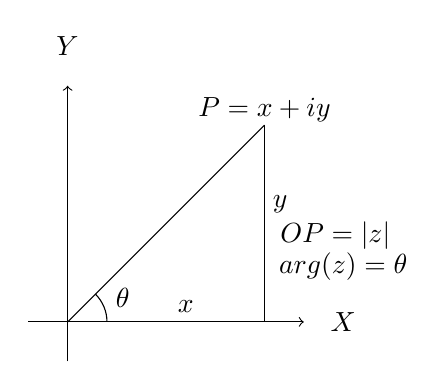
\begin{tikzpicture}
      \draw[->] (-.5,0) -- (3,0);
      \draw[->] (0,-.5) -- (0,3);
      \draw (0, 3.5) node {$Y$};
      \draw (3.5, 0) node {$X$};
      \draw (2.5,0) -- (2.5,2.5);
      \draw (0,0) -- (2.5, 2.5);
      \draw (.5,0) arc(0:45:.5);
      \draw (.7,.3) node{$\theta$};
      \draw (1.5, 0.2) node {$x$};
      \draw (2.7, 1.5) node {$y$};
      \draw (3.4, 1.1) node {$OP=|z|$};
      \draw (3.5, 0.7) node {$arg(z)=\theta$};
      \draw (2.5, 2.7) node{$P=x+iy$};
    \end{tikzpicture}
    \caption{Complex number in argand plane or complex plane}
  \end{center}
\end{figure}

In the diagram, $\theta$ is known as the \textit{argument} of $z$. This is nothing but angle made with positive direction
(i.e. counter-clockwise) of real axis. Now, this argument is not unique. If $\theta$ is an argument of a complex number $z$ then,
$2n\pi + theta$, where $n\in I$, where I is the set of integers. The value of argument for which $-\pi<\theta\leq \pi$ is called
the \textit{principal value} of \textit{argument} or \textit{principal argument}.

\subsection{Different Arguments of a Complex Number}
In the diagram, the argument is given as $\arg(z) = \tan^{-1}\left(\frac{y}{x}\right)$, this value is for when $z$ in first
quadrant. When $z$ will lie in second, third and fourth quadrants the arguments will be
$$\arg(z) = \pi - \tan^{-1}\left(\frac{y}{|z|}\right), arg(z)= -\pi + \tan^{-1}\left(\frac{|y|}{|z|}\right)\text{~and~} arg(z) =
-\tan^P{-1}\left(\frac{|y|}{x}\right)$$
respecticely.

\subsection{Polar Form of a Complex Number}
If $z$ is a non-zero complex number, then we can write $z = r(\cos\theta + i\sin\theta)$, where $r = |z|$ and $\theta = arg(z)$.

In this case, $z$ is also given by $z = r[\cos(2n\pi  \theta) + i\sin(2n\pi + \theta)]$, where $n\in I$.

\subsubsection{Euler's Formula}
The complex number $\cos\theta + i\sin\theta$ is denoted by $e^{i\theta}$ or $c$ is $\theta$, where $c$ is the complex number.

\subsection{Important Results Involving Arguments}
If $z, z_1$ and $z_2$ are complex numbers, then

\begin{enumerate}
\item $arg(\overline{(z)}) = -arg(z)$. This can be easily proven as if $z = x + iy$, then $\overline{z} = x - iy$ i.e. sign of
  argument will get a -ve sign as $y$ gets one.
\item $arg(z_1z_2) = arg(z_1)  + arg(z_2) + 2n\pi$, where
  $$n = \begin{cases}
   0 \text{~if~} & -\pi<arg(z_1)+arg(z_2)\leq-\pi\\
   1 \text{~if~} & -2\pi<arg(z_1)+arg(z_2)\leq-\pi\\
   -1 \text{~if~} & -\pi<arg(z_1)+arg(z_2)\leq2\pi\end{cases}$$
 \item Similarly, $arg(z_1\overline{z_2}) = arg(z_1) - arg(z_2)$.
 \item $|z_1 + z_2| = |z_2 - z_2| \Leftrightarrow arg(z_1) - arg(z_2) = \pi/2$.
 \item $|z_1 + z_2| = |z_1| + |z_2| \Leftrightarrow arg(z_1) = arg(z_2)$.
 \item $|z_1 + z_2|^2 = r_1^2 + r_2^2 + 2r_1r_2\cos(\theta_1 - \theta_2)$.
 \item $|z_1 - z_2|^2 = r_1^2 +r_2^2 + 2r_1r_2\cos(\theta_1 + \theta_2)$.
\end{enumerate}

\section{Vector Representation}
Complex numbers can also be represented as vectors. Length of the vector is nothing but modulus of complex number and argument is
the angle which the vector makes with read axis. It is denoted as $\overrightarrow{OP}$, where $OP$ represents the vector of the
complex number $z$.

\section{Algebraic Operation's Representation}
Let $z_1 = x_1 + iy_1$ and $z_2 = x_2 + iy_2$ be two complex numbers, which are represented by two point $P_1$ and $P_2$ in the
following diagrams.

\subsection{Addition}
Now, as we know that $z_1 + z_2 = (x_1 + x_2) + i(y_1 + y_2)$. Let us see how it looks using geometrically:
\begin{figure}[h]
  \begin{center}
    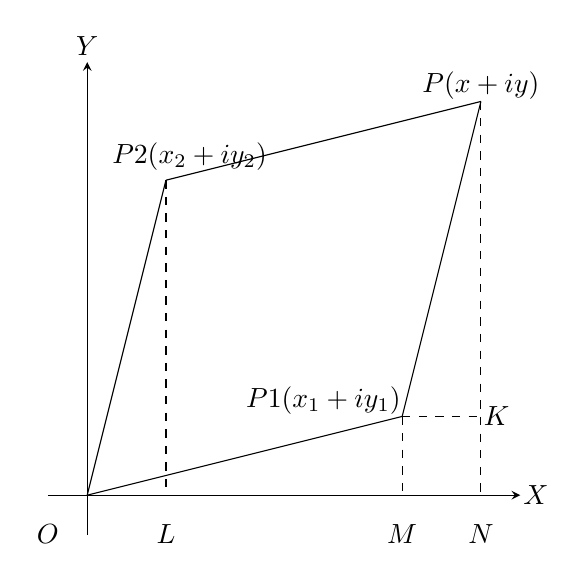
\begin{tikzpicture}
      \draw[->, >=stealth] (-.5,0) -- (5.5,0);
      \draw[->, >=stealth] (0,-.5) -- (0,5.5);
      \draw (5.7, 0) node {$X$};
      \draw (0,5.7) node {$Y$};
      \draw (0,0) -- (4,1);
      \draw (0,0) -- (1,4);
      \draw (1,4) -- (5,5);
      \draw (4,1) -- (5,5);
      \draw[dashed] (4,1) -- (4,0);
      \draw[dashed] (1,4) -- (1,0);
      \draw[dashed] (5,5) -- (5,0);
      \draw[dashed] (4,1) -- (5,1);
      \draw (-.5,-.5) node {$O$};
      \draw (1,-.5) node {$L$};
      \draw (4,-.5) node {$M$};
      \draw (5,-.5) node {$N$};
      \draw (5.2,1) node {$K$};
      \draw (3, 1.2) node {$P1(x_1+iy_1)$};
      \draw (1.3, 4.3) node {$P2(x_2+iy_2)$};
      \draw (5, 5.2) node {$P(x+iy)$};
    \end{tikzpicture}
    \caption{Complex numbers addition}
  \end{center}
\end{figure}
Clearly, $z = z_1 + z_2 = x_1 + x_2 + i(y_1 + y_2)$. Let $P_1M, P_2L$ and $PN$ be parallel to the $y$-axis; $P_1K$ be parallet to
the $x$-axis. This implied that triangle $OP_2L$ and $PP_1K$ are congruent.

We have $P_1K = OL = x_1$ and $P_2L = PK = y_1$

Thus, $ON = OM + MN = OL + P_1K = x_1 + x_2$ and $PN = PK + KN = P_2L + P_1M = y_2 + y_1$

So we can say that coordinates of $P$ are $(x_1 + x_2, y_1 + y_2)$ which represents the complex number $z.$

We also see that this obeys vector addition i.e. $OP_1 + OP_2 = OP_1 + P_1P = OP$

\subsection{Subtraction}
\begin{figure}[h]
  \begin{center}
    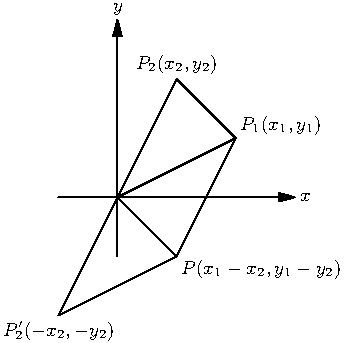
\includegraphics{complex-numbers-subtraction}
    \caption{Complex numbers subtraction}
  \end{center}
\end{figure}
We first represent $-z_2$ by $P_2'$ so that  $P_2P_2'$ is bisected at $O.$ Complete the parallelogram $OP_1PP_2'.$ Then it can be
easily seen that $P$  representd the difference $z_1 - z_2.$

As $OP_1PP_2'$ is a parallelogram so $P_1P = OP_2'.$ Using vetor notation, we have, $z_1 - z_2 = OP_1 - OP_2 = OP_1 + OP_2' = OP_1 + P_1P = P_2P1$

It follows that the complex number $z_1 - z_2$ is represented by the vector $P_1P_2,$ where points $P_1$ and $P_2$ represent the
complex numbers $z_1$ and $z_2$ respectively.

It should be noted that $arg(z_1 - z_2)$ is the angle through which $OX$ must be rotated in the anticlockwise direction to make it
parallel with $P_1P_2.$

\subsection{Multiplication}
\begin{figure}[H]
  \begin{center}
    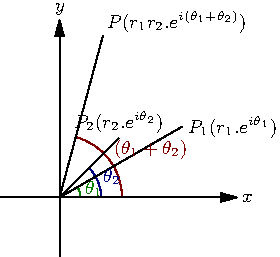
\includegraphics{complex-numbers-multiplication}
    \caption{Complex numbers multiplication}
  \end{center}
\end{figure}
For multiplication it is convenient to use Euler's formula of complex numbers.

Let $z_1 = r_1e^{i\theta_1}$ and $z_2 = r_2e^{i\theta_2},$ then clealry, $z_1z_2 = r_1r_2e^{i(\theta_1 + \theta_2)}$

\chapter{Theory of Equations}
An equation of the form $ax^2 + bx + c = 0$, where $a, b, c\in \mathbb{C}$, the set of complex numbers, is called a \textit{quadratic
  equation}. The numbers $a, b, c$ are called \textit{coefficients} of the equation. The quantity $b^2 - 4ac$ is called the
\textit{discriminant} of the equation. It is represented by $D$ or $\Delta$. A quadratic equation represents a parabola
geometrically.

\noindent\textbf{Examples:}
\begin{enumerate}
\item $4x^2 + 4x + 1 = 0, a = 4, b = 4, c = 1$
\item $7x^3 + 10 = 0$ is not a quadratic equation.
\item $3x^2 -2x^{1/2} + 7 = 0$ is not a quadratic equation.
\item $2x^2 - 4 = 0, a = 2, b = 0, c= -4$
\end{enumerate}

The quadratic equation is called \textit{incomplete} if one of the coefficients $b$ or $c$ is zero. Thus, the last example abpve
represents an incomplete quadratic equation.

An expression of the form $ax^2 + bx + c$ is called a \textit{quadratic expression} while other elements are same as a quadratic
equation.

If two expression in $x$ are equal for all values of $x$ then this statement of equality between the two expression is called an
\textit{identity}.

$f(x) = 0$ is said to be an indentity in $x$ if it is satisfied by all values of $x$ in the domain of $f(x)$. Thus, an indentity in
$x$ is satisfied by all values of $x$ while an equation is satisfied for particular values of $x$.

\noindent\textbf{Example:} $(x + 1)^2 = x^2 + 2x + 1$ is an identity in $x$.

Two equations are called \textit{identical equations} if they have same roots.

\noindent\textbf{Example:} $x^2 - 5x + 4 = 0$ and $2x^2 - 10x + 8 = 0$ are indentical equations because both have same roots $1$ and $4$.

\noindent\textbf{Note:}
\begin{enumerate}
\item Two equations in $x$ are indentical if and only if the coefficients of similar power of $x$ in the two equations are
  proportional. Thus, if $ax^2 + bx + c = 0$ and $a_1x^2 + b_1x + c_1 = 0$ are identical equations, then $\frac{a}{a_1} =
  \frac{b}{b_1} = \frac{c}{c_1}$
\item An equation remains unchanged if it is multiplied or divided by non-zero number.
\end{enumerate}

An expression of the form $a_0x^n + a_1x^{n - 1} + a_2x^{n - 2} + \ldots + a_{n - 1}x + a_0$, where $a_0, a_1, a_2, \ldots, a_n$
are constants $(a_0 \neq 0)$ and $n$ is a positive integer is called a polynomial in $x$ of degree $n$.

As a special case a constant is also called a polynomial of degree zero.

\section{Rational Expression or Rational Function}
An expression of the form $\frac{P(x)}{Q(x)}$, where $P(x)$ and $Q(x)$ are polynomials in $x$, is called a rational expression.

In the particular case, when $Q(x)$ is a non-zero constant, $\frac{P(x)}{Q(x)}$ reduces to a polynomial.Thus, every polynomial is a
rational expression but the converse is not true.

\noindent\textbf{Examples:}
\begin{enumerate}
\item $\frac{x^ - 5x + 4}{x - 2}$
\item $\frac{1}{x - 7}$
\end{enumerate}

\section{Roots of a Quadratic Equation}
The values $x$ for which the equation $ax^2 + bx + c = 0$ are satisfied are called roots of the equation. They are also called
roots of the quadratic expression $ax^2 + bx + c$

Every quadratic equation has at most two roots. Let $ax^2 + bx + c = 0$, where $a\neq 0$

Multiplying both sides of the equation with $a$

$a^2x^2 + abx + ac = 0 \Rightarrow (ax)^2 + 2.ax.\frac{b}{2} + \frac{b^2}{4} + ac - \frac{b^2}{4} = 0$

$\left(ax + \frac{b}{2}\right)^2 = \frac{b^2 - 4ac}{4} \Rightarrow x = \frac{-b \pm\sqrt{b^2 - 4ac}}{2a}$

These are two roots of the quadratic equation. Let us suppose the above quadratic equation has three roots $\alpha, \beta$ and
$\gamma$. These roots will satisfy the above equation. Thus,
$$a\alpha^2 + b\alpha + c = 0, a\beta^2 + b\beta + c = 0, a\gamma^2 + b\gamma + c = 0$$

Subtracting the first two, we get $(\alpha - \beta)[a(\alpha + \beta) + b] = 0$

$\because \alpha \neq \beta \therefore a(\alpha + \beta) + b = 0$

Similarly, $a(\alpha + \gamma) + b = 0$

Subtracting these two, we get $a(\alpha - \gamma) = 0$

$\because a\neq 0 \therefore \alpha = \gamma$

Thus, a quadratic equation has at most two roots.

\section{Sum and Product of the Roots}
From the two obtained  we observe that $\alpha + \beta = -\frac{b}{a}$ and $\alpha\beta = \frac{c}{a}$

\section{Quadratic Expression and its Graph}
Let $f(x) = ax^2 + bx + c$, where $a, b, c\in\mathbb{R}$ and $a\neq 0$.

\begin{equation}
  \label{eq:1}
  f(x) = a\left[\left(x + \frac{b}{2a}\right)^2 + \frac{4ac - b^2}{4a^2}\right]
\end{equation}

\subsection{When a Quadratic Equation is Always Positive/Negative}
It follows from eq. \ref{eq:1}, that $f(x) > 0(< 0)~\forall~x\in\mathbb{R}$ if and only if $a > 0(< 0)$ and $D = b^2 - 4ac <
0$. See Fig. \ref{fig:1}(Fig. \ref{fig:2}). Also, it follows from \ref{eq:1} that $f(x) \geq 0(\leq 0)~\forall~x\in\mathbb{R}$ if
and only if $a > 0(< 0)$ and $D = b^2 - 4ac = 0$. in this case $f(x) < 0(< 0)$ for each $x\in R, x\neq -b/2a$, and the graph of $y
= f(x)$ touches the $x$-axis at $x = -b/2a$.

\begin{figure}[H]
  \begin{center}
    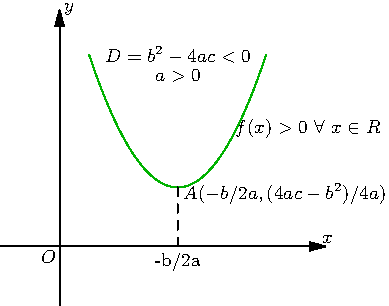
\includegraphics{quadratic-equation-1}
    \caption{When quadratic equation is always positive}
    \label{fig:1}
  \end{center}
\end{figure}

\begin{figure}[H]
  \begin{center}
    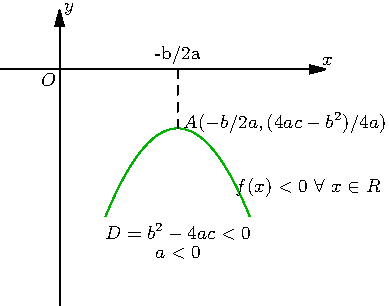
\includegraphics{quadratic-equation-2}
    \caption{When quadratic equation is always negative}
    \label{fig:2}
  \end{center}
\end{figure}

\section{Sign of a Quadratic Equation}
If $D = b^2 - 4ac > 0$, then eq. \ref{eq:1} can be written as

$$f(x) = a\left[\left(x + \frac{b}{2a}\right)^2 - \left(\frac{\sqrt{b^2 - 4ac}}{2a}\right)^2\right]$$
$$= a\left[\left(x + \frac{b + \sqrt{b^2 - 4ac}}{2a}\right)\left(x + \frac{b - \sqrt{b^2 - 4ac}}{2a}\right)\right]$$
$$= a(x - \alpha)(x - \beta)$$

If $D = b^2 - 4ac > 0$ and $a > 0$, then (See Fig. \ref{fig:3})

$$f(x) = \begin{cases}> 0\text{~for~}x <\alpha\text{~or~}x
  >\beta\\>0\text{~for~}\alpha<x<\beta\\=0\text{~for~}x=\alpha,\beta\end{cases}$$

\begin{figure}[H]
  \begin{center}
    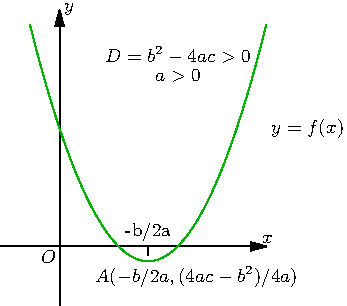
\includegraphics{quadratic-equation-3}
    \caption{When $D > 0$ and $a > 0$}
    \label{fig:3}
  \end{center}
\end{figure}

If $D = b^2 - 4ac > 0$ and $a < 0$, then (See Fig. \ref{fig:4})

$$f(x) = \begin{cases}< 0\text{~for~}x <\alpha\text{~or~}x
  >\beta\\>0\text{~for~}\alpha<x<\beta\\=0\text{~for~}x=\alpha,\beta\end{cases}$$

Note that if $a > 0$, then $f(x)$ attains the least value at $x = -b/2a$, a value which is achieved by differentiating the function
once and at this point the tangent to parabola has slope $0$. The least value is given by
$$f\left(-\frac{b}{2a}\right) = \frac{4ac - b^2}{4a}$$

If $a < 0$, then $f(x)$ is maximum at value $x = -\frac{b}{2a}$ and value of function has the same formula which is for least value
shown above.

\begin{figure}[H]
  \begin{center}
    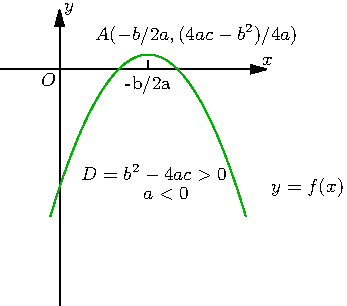
\includegraphics{quadratic-equation-4}
    \caption{When $D > 0$ and $a < 0$}
    \label{fig:4}
  \end{center}
\end{figure}

\section{Position of Roots}
\textbf{Conditions for both roots to be more than a real number $k$}

\begin{figure}[H]
  \begin{center}
    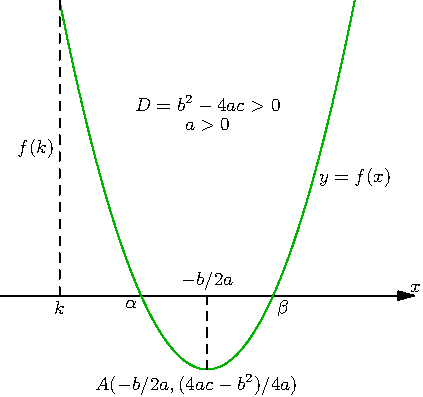
\includegraphics{quadratic-equation-5}
    \caption{When $D > 0$ and $a > 0$}
    \label{fig:5}
  \end{center}
\end{figure}

Form the Fig. \ref{fig:5}, we note that both the roots are more than $k$ if and only if $D>0,~k<-\frac{b}{2a}$ and $f(k)>0$.

In case $a< 0,$ from Fig. \ref{fig:6}, both the roots are more than $k$ if and only if $D>0,~k<-\frac{b}{2a}$ and $f(k)<0$.

\begin{figure}[H]
  \begin{center}
    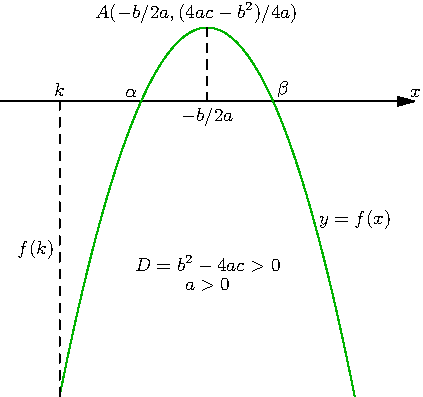
\includegraphics{quadratic-equation-6}
    \caption{When $D > 0$ and $a < 0$}
    \label{fig:6}
  \end{center}
\end{figure}

Combining the above two equations, we get the condition for the roots to be more than a real number $k$ if and only if
$D>0,~k<-\frac{b}{2a}$ and $af(k)>0$. Similarly, condition for the roots to be more than a real number $k$ if and only if
$D>0,~k>-\frac{b}{2a}$ and $af(k)>0$.

\noindent\textbf{Conditions for a real number $k$ to lie between two roots}

Similarly, the real number $k$ lies between the roots of the quadratic equation if and only if $a$ and $f(k)$ are of opposite
signs, i.e. if and only if $a>0,~D>0,~f(k) < 0$ or $a< 0,~D>0,~f(k)>0$.

Combining these two, we get $D>0,~af(k) < 0$ as the condition for $k$ to lie between two roots.

\noindent\textbf{Conditions for exactly one root to lie in between $(k_1, k_2)$ where $k_1<k_2$}

If $a>0$, then exactly one root lies in the interval $(k_1, k_2)$ if and only if $f(k_1)>0$ and $f(k_2)<0$. Also, same is true if
anad only if $f(k_1)<0$ and $f(k_2)>0$. Combining these two we get $f(k_1)f(k_2) < 0$. This condition is also true if $a<0$.

\noindent\textbf{Conditions for both roots to lie in between $(k_1, k_2)$ where $k_1<k_2$}

If $a >0$, both the roots will lies in the interval $(k_1, k_2)$ if and only if $D>0,~k_1<-\frac{b}{2a}<k_2,~f(k_1)>0$ and
$f(k_1)>0$. In case $a<0$, the conditions are $D>0,~k_1<-\frac{b}{2a}<k_2,~f(k_1)<0$ and $f(k_1)<0$.

\noindent\textbf{Conditions for the quadratic equation to have repeated roots}

The quadratic equation $f(x) = ax^2 + bx + c = 0, a\neq 0$ has a repeated root if and only if $f(\alpha) = f'(\alpha) = 0$, where
$\alpha$ is the repeated root. In this case, $f(x) = a(x - \alpha)^2$, In fact, $\alpha = -b/2a$. Geometrically, the $x$-axis will
be a tangent to the parabola at $x = -b/2a$. See Fig. \ref{fig:7} and Fig. \ref{fig:8}.

\begin{figure}[H]
  \begin{center}
    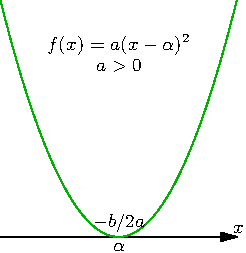
\includegraphics{quadratic-equation-7}
    \caption{$f(\alpha)=0,~f'(\alpha)=0$}
    \label{fig:7}
  \end{center}
\end{figure}

\begin{figure}[H]
  \begin{center}
    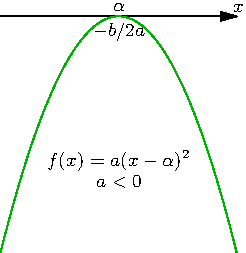
\includegraphics{quadratic-equation-8}
    \caption{$f(\alpha)=0,~f'(\alpha)=0$}
    \label{fig:8}
  \end{center}
\end{figure}

\noindent\textbf{Conditions for two quadratic equations to have one common root}

Consider two quadratic equations $ax^2 + bx + c = 0$ and $a'x^2 + b'x^2 + c' = 0$ having a common root $\alpha$. Clearly, this
common root will satisfy both the equations, i.e. $a\alpha^2 + b\alpha + c = 0$ and $a'\alpha^2 + b'\alpha + c' = 0$.

Solving these two equations, we get

$$\frac{\alpha^2}{bc' - b'c} = \frac{\alpha}{a'c - ac'} = \frac{1}{ab' - a'b}$$
$$\Rightarrow \alpha^2 = \frac{bc' - b'c}{ab' - a'b}, \alpha = \frac{a'c - ac'}{ab' - a'b}$$

Eliminating $\alpha$, we get

$$(a'c - ac')^2 = (bc' - b'c)(ab' - a'b)$$

This is the required condition for two quadratic equations to have one common root.

\begin{figure}[H]
  \begin{center}
    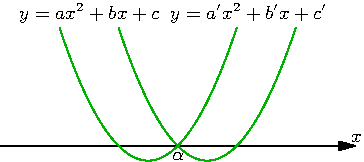
\includegraphics{quadratic-equation-9}
    \caption{Common roots}
    \label{fig:9}
  \end{center}
\end{figure}

\begin{figure}[H]
  \begin{center}
    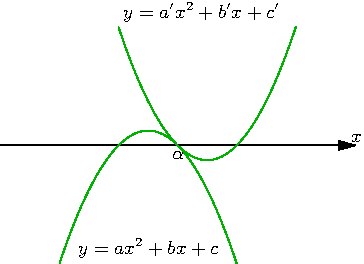
\includegraphics{quadratic-equation-10}
    \caption{Common roots}
    \label{fig:10}
  \end{center}
\end{figure}

To obtain the common root make coefficients of $x^2$ in both the equations same and subtract one equation from the other to obtain
a linear equation in $x$, which you can solve to obtain the common root.

For having both roots common the two equations must be identical i.e. $\frac{a}{a'} = \frac{b}{b'} = \frac{c}{c'}$

\section{General Quadratic Equation in $x$ and $y$}
The general quadratic equation in $x$ and $y$ is given by $ax^2 + 2hxy + by^2 + 2gx + 2fy + c = 0$

$$\therefore x = \frac{-2(hy + g)\pm\sqrt{4(hy + g)^2 - 4a(by^2 + 2fy + c)}}{2a}$$
$$\Rightarrow x + hy + g = \pm \sqrt{(h^2 - ab)y^2 + 2(gh - af)y + g^2 - ac}$$

It can be resolved into two linear factors if $(h^2 - ab)y^2 + 2(gh - af)y + g^2 - ac$ is a perfect square and $h^2 - ab > 0$.

The condition for $(h^2 - ab)y^2 + 2(gh - af)y + g^2 - ac$ to be a perfect square is that its discriminant is $0$, i.e.

$$4(gh - af)^2 - 4(h^2 - ab)(g^2 - ac) = 0$$
$$\Rightarrow abc + 2fgh - af^2 - bg^2 - ch^2 = 0$$

\chapter{Permutations and Combinations}
In this chapter we will study basic principles of counting, permutations and combinations. This study will enable you to further
study the branch of mathematics called combinatorics. You would have certainly encountered a combinatorical problem in your
life. It would be really surprising if you have not. Have you ever solved a Sudoku puzzle or Rubik's cube? Have you ever counted
the number of poker hands that are full houses in order to determine the odds against a full house? Have you ever attempted to
trace through a network without removing your pencil from paper and without tracing any part of network more than once? These are
all combinatorical problems. As you can see that combinatorics has evolved from mathematical games.

With the invention of modern computers, we are enabled to solve more and more problems of combinatorics which were earlier not
feasible due to calculations involved. The computer programs are often based on combinatorical algorithms which determine the speed
and efficiency of the solution. Analysis of these programs and algorithms require sound knowledge of combinatorical mathematics and
thinking. In computer science we write test cases for our programs, and those test cases can be enumerated by applying permutations
and combinations on input data and states produced in the program. Combinatorics is a powerful tool for making sure that the tester
does not miss any test case, which in mission-critical programs is of paramount importance.

The best way to learn combinatorics is to solve a lot of problems. This is in general true for all branches of mathematics but even
more so for combinatorics because a problem which appears simple may be quite difficult to solve or require critical thinking. By
solving problems of different kinds, and by repeating them the concepts will be enforced and discipline will develop.

We start with four basic counting principles and then we will progress into permutations and combinatins. To study the topic of
permutations and combinations it is required to have basic knowledge in set theory which the reader is expected to know.

\section{Four Basic Counting Principles}
Let $S$ be a set. A \textit{partition} of $S$ is a collection of $S_1, S_2, \ldots, S_m$ of subsets of $S$ such that each element
in $S$ is in exactly one of these subsets:
$$S = S_1\cup S_2\cup\ldots\cup S_m$$
$$S_i\cap S_j = \phi(i\neq j)$$
Thus, the sets $S_1, S_2, \ldots, S_m$ are pairwise disjoint sets, and their union is $S$. The subsets $S_1, S_2, \ldots, S_m$ are
called the \textit{parts} of the partition. Note that by this definition a part of the partition may be empty, but usually there is
no advantage in considering partitions with one or more empty sets. The number of objects of a set $S$ is denoted by $|S|$, and is
called the \textit{size} of $S$.

\subsection{Addition Principle}
Suppose that a $S$ is partitioned into pairwise disjoint partys $S_1, S_2, \ldots, S_m$. The number of objects in $S$ can be
determined by finding the number of objects in each of the parts, and adding the numbers so obtained:
$$|S| = |S_1| + |S_2| + \ldots |S_m|$$.
If the sets $S_1, S_2, \ldots, S_m$ are allowed to overlap, then a more profound principle, the inclusion-exclusion principle can
be used to count the number of objects in $S$.

We need to be careful when partitioning $S$ into too many parts. For example, if we partition $S$ into parts in such a way that
each part contains only one element then addition princinple is becomes counting the number of parts, which is basically same as
listing all objects of $S$. Thus the art of applying addition princinple is to partition the set $S$ into not too many parts.

\noindent\textbf{Example:} In a university there are four mathematics courses, two economics courses, and three lietrature
courses. A student is allowed to enroll into one course at most. Thus, we see that a student can take a course in $4 + 2 + 3 = 9$
ways.

Next principle is multiplication principle which will be stated for two sets, but it can be generalized to any finite number of
sets.

\subsection{Multiplication Principle}
Let $S$ be a set of ordered pairs $(a, b)$, where the first object comes from a set of size $p$, and for each choice of object $a$
there are $q$ choices for object $b$. Then the size of $S$ is $p\times q$:
$$|S| = p\times q$$
As in basic arithmetic multiplication is repeated addition, similarly multiplication principle is actuallly a consequence of the
addition principle i.e. repeated addition. Let $a_1, a_2, \ldots, a_p$ be $p$ different choices for the object $a$. We partition
$S$ into parts $S_1, S_2, \ldots, S_p$ where $S_i$ is the set of ordered pairs in $S$ with first object $a_i(i = 1, 2, \ldots,
p)$. The size of each $S_i$ is $q$; hence, by the addition principle,
$$|S| = |S_1| + |S_2| + \ldots + |S_p|$$
$$= q + q + \ldots + q(p q'\text{s})$$
$$= p\times q$$
The multiplication principle can be stated in another way as: If a first task has $p$ outcomes, and no matter what the outcome of of
the first task, a second task has $q$ outcomes i.e. outcomes for two tasks are mutually exclusive, then the two tasks can be
performed in $p\times q$ outcomes.

\noindent\textbf{Example:} Pencil comes in two different lengths, four different hardness, and three different thickness. How many
different types of pencils are there?

The pencil has three different properties, which are exclusive of each other, and thus, we can apply multiplication
principle. Hence, number of different types of pencils is $2\times4\times3 = 24$.

\noindent\textbf{Example:} The number of ways a man, woman, boy, and girl can be selected from three men, three women, five boys and
four girls is $3\times3\times5\times4 = 180$.

\noindent\textbf{Example:} Determine the number of positive integers that are factors of the number
$$2^3\times3^4\times5^5\times7^7$$
The numbers $2, 3, 5,$ and $7$ are prime numbers. By the fundamental theorem of arithmetic, each factor is of the form
$$2^i\times3^j\times5^k\times7^l$$
where $0\leq i\leq2, 0\leq j\leq3, 0\leq k\leq5,$ and $0\leq l\leq7$. There are three choices for $i$, four for $j$, six for $k$, and
eight for $l$. By multiplication principle, the number of factors is $3\times4\times6\times8 = 576$.

In the multiplication principle the $q$ choices for object $b$ may vary with the choices of $a$. The only requirement is that there
be the same number $q$ of choices, not necessarily the same choices.

\noindent\textbf{Example:} How many two-digit numbers have distinct, and nonzero digits?

A two-digit number $ab$ can be regarded as an ordered pair $(a, b)$, where $a$ is the tens digit, and $b$ is the units digit. Both
are not allowed to be $0$, and they must be different. Thus, we see that there are $9$ ways to choose $a$, which are $1, 2, \ldots,
9$. Once $a$ is chosen we cannot use the same digit for $b$, which means we are left with $8$ choices for $b$. Here we see that
choice of $a$ makes a difference on what choices $b$ has. However, for multiplication principle to be applicable what matters is
that the number of choices remain constant which is $8$ in this case. Applying multiplication principle, we arrive at the answer of
the question as $9\times8 = 72$.

There is another way to arrive at the same result. Total number of two-digit number is $90, 10,11, 12, \ldots, 99$. Of these $90$
numbers $9$ have a zero in them$(10, 20, 30, \ldots, 90)$, and $9$ have repeated digits$(11, 22, \ldots, 99)$. Thus, total number of
required numbers equals $90 - 9 - 9 = 72$.

We can derive two important ideas from the previous example. First is that it is possible to solve a counting problem in many
ways. The second idea is that to find the number of objects in a set $A$ (in this csae the set of two-digit numbers with nonzero,
and distinct digits) it may be easier to find the number of objects in a larger set $U$ containing $S$ (the set of all
two-digit numbers), and then subtract the number of objects of $U$ that do not belong to $A$ (the two-digit numbers containing $0$
or repeated digit). This leads us to subtraction principle.

\subsection{Subtraction Principle:}
Let $A$ be a set, and let $U$ be a larger set containing $A$. Let
$$\overline{A} = U\textbackslash A = \{x\in U: x\notin A\}$$
be the complement of $A$ in $U$. Then the numebr $|A|$ of object in $A$ is given by the rule
$$|A| = |U| - |\overline{A}|$$

The set $U$ is usually some natural set containing all the objects under discussion (it is called \textit{universal set}). Using
the subtraction principle should be used only if it is easier to count the number of object in $U$ nd $\overline{A}$ tha to count the
number of objects in $A$.

\noindent\textbf{Example:} Most websites on internet have a lower limit of $8$ characters as password length. Suppose if these
passwordss are to made up of the digits $0, 1, 2, \ldots, 9$, and the lowercase letters $a, b, c, \ldots, z$ then how many passwords
will have a repeated symbol?

There are a total of $10$ digits, and $26$ letters i.e. 36 symbols. So by two applications of multiplication principle, we get
$$|U| = 36^8 = 2,821,109,907,456$$
and
$$|\overline{A}| = 36.35.34.33.32.31.30.29 = 1,220,096,908,800$$
Therefore,
$$|A| = |U| - |\overline{A}| = 1,601,012,998,656$$.

Now we will formulate the last principle of counting principles.

\subsection{Division Principle}
Let $S$ be a finite set that is partitioned into $k$ parts in such a way that each part contains the same number of objects. Then
the number of parts in the partition is given by the rule
$$k = \frac{|S|}{\text{number of objects in a part}}$$

\noindent\textbf{Example;} There are $240$ rats in a collection of cages. If each cage contains $2$ rats, the number of cages
equals $$\frac{240}{2} = 120$$.

Interesting problems of division principle will be found in the problems section.

Most counting problems can be classified as one of the following types:

\begin{enumerate}
\item Count the number of ordered arrangements or ordered selection of objects
  \begin{enumerate}
  \item without repeating any object,
  \item with repetion(perhaps limited) of objects permitted.
  \end{enumerate}
\item Count the number of unordered arrangements or unordered selection of objects
  \begin{enumerate}
    \item without repeating any object,
  \item with repetion(perhaps limited) of objects permitted.
  \end{enumerate}
\end{enumerate}

We can represent repetition, and nonrepetition of objects as selection from a set, and a multiset. The latter might prove to be more
useful in some cases. A \textit{multiset} is like a set except that its members need not be distinct.\footnote{Thus, a cardinal
rule of sets is broken by multisets because a set is not supposed to have duplicates or repeated elements. The set $\{a, a, b\}$ is
same as the set $\{a, b\}$ but not so for multisets} For example, a multiset $M$ with three $a$'s, two $b$'s i.e. $5$ elements of
$2$ different types. We usually indicate a multiset by specifying the number of times different types of elements occur in
it. Thus, $M$ is denoted by $\{3.a,2.b\}$.\footnote{In standard set-theory's notation, we could denote the multiset $M$ using
ordered pairs as $\{(a, 3), (b, 2)\}$}. The numbers $3$, and $2$ are the \textit{repetition members} of the multiset $M$. Thus we
can extrapolate that a set is a multiset with all repetition numbers equal to $1$. Often there is no limit on number of repetitions
i.e. infinite repetitions are allowed.\footnote{In no circumstance, we need to consider different sizes of $\infty$.}

\section{Factorial of $n$}
Factorial of $n$ is denoted by $n!$. In the old style it is written as $\oldfact{n}$. $n!$ is given by the first $n$ natural
numbers, i.e. $$n! = 1.2.3.4\ldots(n - 1).n$$ Also, $0! = 1$, which we will prove later.

Permutation means arrangement of objects along with selection. In the permutation of object order matter. If order of object
changes then their permutation also changes. Combination of objects means selection of objects in such a way that order does not
matter.

\section{Permutation of Sets}
Let $r\in \mathbb{P}$. By an $r$-\textit{permutation} of a set $S$ of $n$ elements has a meaning of an ordered(by definition of
permutation) arrangement of $r$ of the $n$ elements$(r\leq n)$. If $S = \{a, b, c\},$ then the three $1$-permutations of $S$ are
$$a~~~b~~~c,$$
the six $2$-permutations of $S$ are
$$ab~~~ac~~~ba~~~bc~~~ca~~~cb,$$
and the six $3$-permutations of $S$ are
$$abc~~~acb~~~bac~~~bca~~~cab~~~cba.$$

There are no $4$-permutations of $S$ because that will violate the assumption that $r\leq n$.

The $r$-permutations of an $n$-element set is denoted by $P(n, r)$ or ${}_nP_r$ or ${}^nP_r$. If $r > n$ then ${}^nP_r =
0$. Clearly, ${}^nP_1 = n$ for each $n\in \mathbb{P}$.

For $n$ and $r$ positive integers with $r\leq n,$ $${}^nP_r = n\times(n - 1)\times\ldots\times(n - r + 1).$$

Permutation of $n$ objects taken $r$ at a time is equivalent ot filling $r$ different vacant spots from $n$ different objects. We
can fill first spot by $n$ ways, second spot can be filled by remaining objects i.e. $n - 1$ ways, and proceeding this way we find
that $r$th spot can be filled in $n - r + 1$ ways. Thus total number of ways is $$n\times(n - 1)\times\ldots(n - r + 1)$$.

We can rewrite the above as $$\frac{n\times(n - 1)\ldots(n - r + 1)\times(n - r)\times\ldots2\times 1}{(n - r)\times(n - r -
  1)\times\ldots2\times1}$$
$${}^nP_r = \frac{n!}{(n - r)!}$$

Alternatively, first place can be filled in $n$ ways. Rest of $r - 1$ spots from $n - 1$ objects can be filled in ${}^{n - 1}P_{r -
1}$ ways. Thus, ${}^nP_r = n.{}^{n - 1}P_{r - 1}$. Similarly, ${}^{n - 1}P_{r - 1} = (n - 1).{}^{n - 2}P_{r - 2}$. Proceeding this
way we find that ${}^{n - r + 1}P_1 = n - r + 1$. Multiplying and cancelling common factors, we get ${}^nP_r = n\times(n -
1)\times\ldots\times(n - r + 1).$

The number of permutations of $n$ elements is ${}^nP_n = \frac{n!}{0!} = n!$. If we follow first result then it is evident that $0!
= 1.$

\subsection{Meaning of $\frac{1}{(-k)!}, k\in\mathbb{P}$}
We have ${}^nP_r = \frac{n!}{(n - r)!}$. Putting $r = n + k$, we have ${}^nP_{n + k} = \frac{n!}{(-k)!}$. But the number of ways of
arranging $n + 1$ objects out of $n$ different objects $= 0 \Rightarrow \frac{1}{(-k)!} = 0.$

\noindent\textbf{Note:} Although $(-k)!$ has no meaning by the definition of factorial but if we consider the above result then the
formula for permutation becomes valid even for $r > n.$

\subsection{Circular Permutation}
Let us consider arranging objects along a circle. Let us consider that four persons $A, B, C,$ and $D$ are sitting around a table. We
can have following arrangements:

\begin{center}
  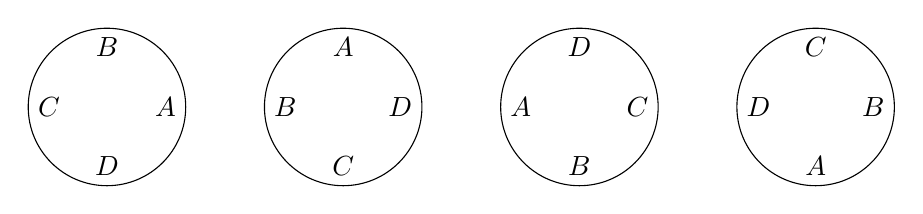
\begin{tikzpicture}
    \draw (0,0) circle (1cm);
    \draw (3cm,0) circle (1cm);
    \draw (6cm,0) circle (1cm);
    \draw (9,0) circle (1cm);
    \draw (1cm, 0) node[anchor=east] {$A$};
    \draw (0, 1cm) node[anchor=north] {$B$};
    \draw (-1cm, 0) node[anchor=west] {$C$};
    \draw (0, -1cm) node[anchor=south] {$D$};
    \draw (4cm, 0) node[anchor=east] {$D$};
    \draw (3cm, 1cm) node[anchor=north] {$A$};
    \draw (2cm, 0) node[anchor=west] {$B$};
    \draw (3cm, -1cm) node[anchor=south] {$C$};
    \draw (7cm, 0) node[anchor=east] {$C$};
    \draw (6cm, 1cm) node[anchor=north] {$D$};
    \draw (5cm, 0) node[anchor=west] {$A$};
    \draw (6cm, -1cm) node[anchor=south] {$B$};
    \draw (10cm, 0) node[anchor=east] {$B$};
    \draw (9cm, 1cm) node[anchor=north] {$C$};
    \draw (8cm, 0) node[anchor=west] {$D$};
    \draw (9cm, -1cm) node[anchor=south] {$A$};
  \end{tikzpicture}
\end{center}

As shown four persons are sitting around a round table, and four anticlockwise rotations have lead to four arrangements. But if
$A,B,C,D$ are sitting in a row, and then are shiftedd such that last occupies the place of first, then the four arrangements will be
different. Thus, if there are $n$ objects then for each circular arrangement there are nn linear arrangements. But for $n$ different
objects total number of linear arrengements are $n!$ so the total number of circular arrangements are $$\frac{n!}{n} = (n - 1)!$$.

Thus, we can say that number of circular $r$-permutations of a set of $n$ elements is given by $$\frac{{}^nP_r}{r} = \frac{n!}{r.(n
  - r)!}$$

\subsection{Clockwise and Anti-Clockwise Arrangements}
When clockwise and anticlockwise arranegemnts are same then total number of permutations will become half of what we computed in
previous case i.e. $$\frac{{}^nP_r}{2r} = \frac{n!}{2r.(n - r)!}$$

\section{Combination of Sets}
Consider a set $S$ having $n$ elements. A \textit{combination} of a set $S$ has a meaning of an unordered selection of the elements
of $S$. The result of each selection is a \textit{subset} $A$ of the elements of $S: A\subset S$. Thus, the terms
\textit{combination} and \textit{subset} are interchangeable.

Now let $r$ be a nonnegative integer. By an $r$-\textit{combination} of a set $S$ of $n$ elements, we understand an unordered
selection of $r$ of the $n$ objects of $S$. The result will be an $r$-subset of $S$.

If $S = \{a, b, c, d\},$ then $$\{a, b, c\}, \{a, b, c\}, \{a, c, d\}, \{b, c, d\}$$ are the four $3$-subsets of $S$. We denote
the number of $r$-subsets or $r$-combinations of an $n$-element set by ${n\choose r}$ or ${}_nC_r$ or ${}^nC_r$. Obviously,
$${n\choose r} = 0~~~~~~\text{if~}r > n.$$
Also,
$${0\choose r} = 0~~~~~~\text{if~}r > 0.$$

The following facts are easy to figure out for each nonnegative integer $n$ $${0\choose 0} = {n\choose 0} = {n\choose n} = 1, {n\choose 1} = n,$$

For $0\leq r\leq n,$ $${}^nP_r = r!{}^nC_r.$$
Hence,
$${}^nC_r = \frac{n!}{r!(n - r)!}$$

Let $S$ be an $n$-element set. Each $r$-permutation of $S$ arises from following tasks
\begin{enumerate}
\item Choose $r$ elements from $S$.
\item Arrange the chose $r$ elements in some order.
\end{enumerate}

The number of ways to carry out first task, by definition, is ${}^nC_r$. The number of ways to carry out second task is ${}^nP_r =
r!$. By the multiplication principle, we have ${}^nP_r = r!{}^nC_r$. Now applying the formula for permutations, we have
$${}^nC_r = \frac{n!}{r!(n - r)!}.$$

\section{Permutation of Multisets}
Let $S$ be a multiset with objects of $k$ different types, where each object can be repeated infinitely. Then the number of
$r$-permutations of $S$ is $k^r$.

To prove this, we can choose the first item to be an object of any one of the $k$ types. Since the number of repetitions are
infinite the second item can be also chose in $k$ ways. In fact, any item can be chosen in $k$ ways due to infinite
repetition. Following, multiplication principle, total number of such permutations is $k^r$.

Let $S$ be a multiset with objects of $k$ different types with finite repetition numbers $n_1, n_2, \ldots, n_k$ respectively. Let
the size of $S$ be $n = n_1 + n_2 + \ldots + n_k.$ Then the number of permutations of $S$ equals $$\frac{n!}{n_!!n_2!\ldots
  n_k!}.$$

We can calculate this by thinking in terms of $n$ places, and we want to put exactly one of the objects of $S$ in each of the
places. We have $n_1$ objects of one type in $S$, so we must choose a subset of $n_1$ places from the set of $n$ places. We can do
this in ${}^nC_{n_1}$ ways. After this we have $n - n_1$ places left, and we have $n_2$ objects of second type. So following
similarly we can do this in ${}^{n - n_1}C_{n_2}$ ways. Following this way invoking multiplication principle, the number of
permutations of $S$ equals
$${}^nC_{n_1}.{}^{n - n_1}C_{n_2}.{}^{n - n_1 - n_2}C_{n_3}\ldots{}^{n - n_1 - n_2 - \ldots - n_{k - 1}}C_{n_k}$$
which gives
$$\frac{n!}{n_1!(n - n_1)!}.\frac{(n - n_1)!}{n_2!(n - n_1 - n_2)!}.\frac{(n - n_1 - n_2)!}{n_3!(n - n_1 - n_2 -n_3)!}\ldots
\frac{(n - n_1 - n_2 - \ldots - n_{k - 1})!}{n_k!(n - n_1 - n_2 - \ldots - n_k)!}$$
which after cancellation, reduces to
$$\frac{n!}{n_1!n_2!\ldots n_k!}$$

Let $n$ be a positive integer, and let $n_1, n_2, \ldots, n_k$ be positive integers with $n = n_1 + n_2 + \ldots + n_k$. The number
of ways to partition a set of $n$ objects into $k$ labeled boxes in which Box 1 contains $n_1$ objects, Box 2 contains $n_2$
objects, $\ldots$, Box $k$ contains $n_k$ objects equals
$$\frac{n!}{n_1!n_2!\ldots n_k!}.$$

If the boxes are not labeled, and $n_1 = n_2 = \ldots = n_k$, then the number of partitions equals $$\frac{n!}{k!n_1!n_2!\ldots
  n_k!}.$$

We can calculate this by direct application of the multiplication principle. So we first choose $n_1$ objects for the first box,
then $n_2$ of the remaining $n - n_1$ objects for the second box and so on. By the multiplication principle, the number of ways is
$${}^nC_{n_1}.{}^{n - n_1}C_{n_2}.{}^{n - n_1 - n_2}C_{n_3}\ldots{}^{n - n_1 - n_2 - \ldots - n_{k - 1}}C_{n_k}$$
which is same as the last result, i.e.
$$\frac{n!}{n_1!n_2!\ldots n_k!}$$

If boxes are not labeled and $n_1 = n_2 = \ldots = n_k,$ then the result has to be divided by $k!$ because for each way of
distributing the objects into the $k$ unalbeled boxes there are $k!$ ways in which we can attach the labels to the boxes. Thus,
using the division principle, we arrive at the result as
$$\frac{n!}{n_1!n_2!\ldots n_k!}.$$

\section{Combination of Multisets}
If $S$ is a multiset, then an $r$-combination of $S$ is an unorndered selection of $r$ of the objects of $S$. Thus, an
$r$-combination of $S$ is itslef a multiset, a \textit{submultiset} of $S$ of size $r$, or, for short, an $r$-submultiset. If $S$
has $n$ objects, then there is only one $n$-combination of $S$, namely, $S$ itself. If $S$ contains objects of $k$ different types,
then there are $k 1$-combinations of $S$.

Let $S$ be a multiset with objects of $k$ types, each with an infinite repetitions, then the number of $r$-combinations of $S$
equals
$${}^{r + k - 1}C_r = {}^{r + k - 1}C_{k - 1}.$$

Let $k$ types of objects of $S$ be $a_1, a_2, \ldots, a_k$ so that
$$S = \{\infty.a_1, \infty.a_2, \ldots, \infty.a_k\}$$

Any $r$-combination of $S$ is of the form $\{x_1.a_1, x_2.a_2, \ldots, x_k.a_k\}$, where $x_1, x_2, \ldots, x_k$ are nonnegative
integers with $x_1 + x_2 + \ldots + x_k = r$. The converse is also true. Thus, the number of $r$-combinations of $S$ equals the
number of solutions of the equation $$x_1 + x_2 + \ldots + x_k = r.$$

We will show that the number of solutions of this equation is given by number of permuations of the multiset
$$T = \{r.1, (k - 1).*\}$$
of $r + k - 1$ objects of two different types. Given a permuation of $T,$ the $k - 1 *$'s divide the $r 1$s into $k$ groups. Let
there be $x_1 1$s to the left of the first $*, x_2 1$s between the first and second $*,\ldots,$ and $x_k 1$s to the right of last
$*$. Clearly, $x_1 + x_2 + \ldots + x_k = r$. The converse of this is also true. Thus, required combination is given by the
formula $${}^{r + k - 1}C_r = {}^{r + k - 1}C_{k - 1}.$$

\section{Some Important Indentities}
\begin{enumerate}
\item ${}^nP_r = r.{}^{n - 1}P_{r - 1} + {}^{n - 1}P_r$.
\item ${}^nC_r = {}^nC_{n - r}$.
\item ${}^nC_{r - 1} + {}^nC_r = {}^{n + 1}C_r$.
\item ${}^nC_r = {}^nC_s \Rightarrow r = s$ or $r + s = n$.
\item ${}^nC_r = \frac{n - r + 1}{r}.{}^nC_{r - 1}~(1\leq r\leq n)$.
\item If $n$ is even, then the greatest value of ${}^nC_r$ is ${}^nC_m$, where $m = n/2$. If $n$ is odd, then the greatet value is
  ${}^nC_m$, where $m = (n - 1)/2$ or $m = (n + 1)/2$.
\item If $n = 2m + 1$, then ${}^nC_0 < {}^nC_1 < {}^nC_2 < \ldots < {}^nC_m = {}^nC_{m + 1}$. ${}^nC_{m + 1} > {}^nC_{m + 2} >
  \ldots > {}^nC_n$.
\item If $n = 2m + 1$, then ${}^nC_0 < {}^nC_1 < {}^nC_2 < \ldots <{}^nC_m > {}^nC_{m + 1} > {}^nC_{m + 1} > \ldots > {}^nC_n$.
\item ${}^nC_0 + {}^nC_1 + {}^nC_2 + \ldots + {}^nC_n = 2^n$.
\item ${}^nC_0 + {}^nC_1 + {}^nC_2 + \ldots = {}^nC_1 + {}^nC_3 + \ldots = 2^{n -1}$.
\item ${}^{2n + 1}C_0 + {}^{2n + 1}C_1 + \ldots + {}^{2n + 1}C_n = {}^{2n + 1}C_{n + 1} = {}^{2n + 1}C_{n + 1} + {}^{2n + 1}C_{n +
  2} + \ldots + {}^{2n + 1}C_{2n + 1} = 2^{2n}$.
\item $r.{}^nC_r = n.{}^{n - 1}C_{r - 1}$.
\end{enumerate}

\section{Some Useful Results}
Number of selections of $r$ objects out of $n$ different objects:

\begin{enumerate}
\item When $p$ paticular objects are always included $= {}^pC_p.{}^{n - p}C_{r - p} = {}^{n - p}C_{r - p}$.
\item When $p$ paticular objects are excluded $= {}^{n - p}C_r$.
\item Number of selections of $r$ objects out of $n$ different objects such that $p$ particular objects are not together in any
  selection $= {}^nC_r = {}^{n - p}C_{r - p}$.
\item Number of selection of $r$ consecutive objects out of $n$ objects in a row $= n - r + 1$.
\item Number of selection of $r$ consecutive objects out of $n$ objects along a circle $= n$ when $r < n, 1$ when $r = n$.
\item Number of selections of zero or more objects out of $n$ different objects $= {}^nC_0 + {}^nC_1 + {}^nC_2 + \ldots + {}^nC_n =
  2^n$.
\item Number of selections of one or more objects out of $n$ different objects $= {}^nC_1 + {}^nC_2 + \ldots + {}^nC_n = 2^n - 1$.
\item Number of selections of zero or more objects out of $n$ identical objects $= n + 1$.
\item Number of selections of one or more objects out of $n$ identical objects $= n$.
\item Number of selection of one or more objects from $(p + q + r)$ objects, out of which $r$ objects are identical and of one
  type, $q$ objects are identical and of second type, $r$ objects are identical and of third type $= (p + 1)(q + 1)(r + 1) - 1$.
\item Number of selection of one or more objects from $(p + q + r + n)$ objects, out of which $r$ objects are identical and of one
  type, $q$ objects are identical and of second type, $r$ objects are identical and of third type and rest $n$ are different $= (p
  + 1)(q + 1)(r + 1)({}^nC_0 + {}^nC_1 + {}^nC_2 + \ldots + {}^nC_n) - 1 = (p + 1)(q + 1)(r + 1)2^n - 1$
\item Number of ways of distributing $n$ different objects among $3$ persons such that they gey $x, y, z$ objects $= {}^nC_x.{}^{n
  - x}C_y.{}^{n - x - y}C_z.3! = \frac{n!}{x!y!z!}.3!$.
\item Number of ways of distributing $n$ different objects in $5$ sets having $a, b, c, d, e$ objects$(a + b + c + d + d = n)$:
  \begin{enumerate}
  \item When two sets have equal number of objects and three sets have equal number of objects $= \frac{n!}{a!b!c!d!e!2!3!}$
  \item When all sets have equal number of objects $= \frac{n!}{a!b!c!d!e!5!}$
  \end{enumerate}
\item Number of ways of distributing $n$ different objects among $5$ persons
  \begin{enumerate}
  \item When all person get different number of objects $= \frac{n!}{a!b!c!d!e!}.5!$.
  \item When two persons get equal number of objects and three get equal number of objects $= \frac{n!}{a!b!c!d!e!2!3!}.5!$.
  \item When all get equal number of objects $= \frac{n!}{a!b!c!d!e!5!}.5! = \frac{n!}{a!b!c!d!e!}$.
  \end{enumerate}
\end{enumerate}

\section{Permutations with Repetitions}
The objective is to find permutation of $r$ objects out of $n$ objects of which $p$ are of one type, $q$ of second type and so on.

Let the different objects be denoted by $a, b, c, \ldots$

Consider the product $$\left(1 + \frac{ax}{1!} + \frac{a^2x^2}{2!} + \ldots + \frac{a^px^p}{p!}\right)\left(1 + \frac{bx}{1!} +
\frac{b^2x^2}{2!} + \ldots + \frac{b^qx^q}{q!}\right)\ldots$$

Required number of permutations $=$ sum of all possible terms of the form $= \frac{r!}{p!q!\ldots}a^pb^q\ldots$ where $p + q + \ldots
= r$

$= r!$. coeff. of $x^r$ in $\left[\left(1 + \frac{x}{1!} + \frac{x^2}{2!} + \ldots + \frac{x^p}{p!}\right)\left(1 + \frac{x}{1!} +
\frac{x^2}{2!} + \ldots + \frac{x^q}{q!}\right)\ldots\right]$

\section{Combinations with Repetitions}
The objective is to find combinations of $r$ objects out of $n$ objects under different cases of repetitions. To begin with we
consider combinations of $r$ objects taken out of $n$ objects of which $p$ are of one type, $q$ of the second type and so on.

Let the different things be denoted by the letters $a, b, \ldots$

Consider the product $(1 + ax + a^2x^2 + \ldots + a^px^2)(1 + bx + b^2x^2 + \ldots + b^qx^2)\ldots$ All the terms in the product
is of the same degree in the letters $a, b, \ldots$ as in $x$. The coefficient of $x^r$ in the product is the number of ways of
taking $r$ of the letters $a, b, \ldots$ with the restriction that maximum number of $a$'s is $p$, maximum number of $b$'s is $q$ and so
on. Coeff. of $x^r$ will not change if $a = b = \ldots = 1$. Thus required number of combinaitons = Coeff. of $x^r$ in $(1 + x + x^2 +
\ldots + x^2)(1 + x + x^2 + \ldots + x^2)\ldots$

Similarly, number of combinaitons of $r$ objects out of $n$ objects of which $p$ are of one type, $q$ are of second type and $(n -
p - q)$ things are all different $=$ Coeff. of $x^r$ in $[(1 + x + x^2 + \ldots + x^p)(1 + x + x^2 + \ldots + x^q)(1 + x)(1 +
  x)\ldots \text{~to~} (n - p - q)\text{factors~}]$

$=$ Coeff. of $x^r$ in $[(1 + x + x^2 + \ldots + x^p)(1 + x + x^2 + \ldots + x^q)(1 + x)(1 + x)^{n - p - q}]$

Similarly, number of combinations of $r$ objects out of $n$ objects of which $p$ are of one type, $q$ are of second type and so on,
when each thing is taken at least once $=$ Coeff. of $x^r$ in $[(x + x^2 + \ldots + x^p)(x + x^2 + \ldots + x^q)\ldots]$

$=$ Coeff. of $x^{r - 3}$ in $[(1 + x + x^2 + \ldots + x^p)(1 + x + x^2 + \ldots + x^q)$

If $n$ is a negative integer, then $(1 + x)^n = 1 + \frac{n}{1!}x + \frac{n(n - 1)}{2!}x^2 + \ldots\text{~to~}\infty$ [this comes
  from binomial theorem]

So if $n$ is a positive inetger then $(1 + x)^{-n} = 1 + \frac{n}{1!}x + \frac{n(n + 1)}{2!}x^2 + \ldots\text{~to~}\infty$

Coeff. of $x^r$ in $(1 - x)^{-n} = {}^{n + r - 1}C_r$ which is number of ways in which $r$ identical objects can be distributed
among $n$ persons can get zero of more objects $=$ Coeff. of $x^r$ in $(1 + x + \ldots + x^r)^n = \left(\frac{1 - x^{r + 1}}{1 -
    x}\right)^n = [(1 - x^{r + 1})(1 - x)^{-n}]$.

$=$ Coeff. of $x^r$ in $(1 - x)^{-n}$ (leaving powers higher than $x^r$) $= {}^{n + r - 1}C_r$.

\section{Integral Solutions of Equations}
As we have proved earlier, for equation $x_1 + x_2 + \ldots + x_r = n$ is equivalent of distributing $r$ identical objects among
$n$ persons when each person getting zero or more things $= {}^{n + r - 1}C_r$

Similarly, number of non-negative integral solutions of equation $x + 2y + 3z + 4w = n$, equals coeff. of $x^n$ in $[(1 - x)^{-1}(1
  - x)^{-2}(1 - x)^{-3}(1 - x)^{-4}]$.

Similarly, number of positive integral solutions of equation $x + 2y + 3z + 4w = n$, equals coeff. of $x^{n -(1 + 2 + 3 + 4})$ in
$[(1 - x)^{-1}(1 - x)^{-2}(1 - x)^{-3}(1 - x)^{-4}]$.

\section{Geometrical Applications of Combinations}
Some basic geometrical results involving combinations are given below:
\begin{enumerate}
\item $n$ non-concurrent and non-parallel straight lines, points of intersection are ${}^nC_2$.
\item The number of straight lines constructed out of $n$ points, when no three points are collinear, are ${}^nC_2$.
\item Given $n$ points, if $m$ are collinear, then number of straight lines possible are ${}^nC_2 - {}^mC_2 + 1$.
\item In a polygon, total number of diagonals out of a $n$ points, when no three points are collinear, are $\frac{n(n - 3)}{2}$.
\item Number of triangles formed from $n$ points, when no three points are collinear, are ${}^nC_3$.
\item Number of triangles formed out of $n$ points in which $m$ are collinear, ${}^nC_3 - {}^mC_3$.
\item Number of triangles constructed out of $n$ points, when none of the side is common with the sides of polygon, are ${}^nC_3 -
  {}^nC_1 - {}^nC_1.{}^{n - 4}C_1$.
\item Number of parallelogram constructed by two system of parallel lines, when first set contains $m$ parallel lines and second
  set contains $n$ parallel lines, are ${}^nC_2\times{}^mC_2$.
\item Number of squares formed by two system of parallel lines in which first set is perpendicular to second set of lines, when
  first set contains $m$ parallel lines and second set contains $n$ parallel lines is $\displaystyle\sum_{r=1}^{m - 1}(m - r)(n -
  r);~m<n$.
\end{enumerate}

\section{Number of Divisors and Sum of Divisors}
Let $n = p_1^{n_1}.p_2^{n_2}\ldots p_n^{n_k}$ where $p_1, p_2, \ldots, p_k$ are distinct prime numbers and $n_1, n_2, \ldots,
n_k\in \mathbb{P}$. Obvously, any divisor of $n$ is of the form $d = p_1^{m_1}.p_2^{m_2}\ldots p_k^{m_k}$ where $m_1, m_2,
\ldots\in\mathbb{N}$ such that $0\leq m_i\leq n_i, i = 1, 2, \ldots, k$. Therefore, the total no. of divisors for $n$ will be equal
to the number of ways of selecting at least one from $n_1$ identical prime numbers $p_1, n_2$ primes $p_2$ and so on. The number of
such ways is $$(n_1 + 1)(n_2 + 1)\ldots(n_k + 1)$$. These divisors will also include $1$ and $n$, so obviously, number of divisors
other than $1$ and $n$ is $$(n_1 + 1)(n_2 + 1)\ldots(n_k + 1) - 2$$

The sum of all divisors for $n$ is given by $$\sum_{r_1=0}^{n_1}\sum_{r_2=0}^{n_2}\ldots\sum_{r_k=0}^{n_k}
p_1^{r_1}p_2^{r_2}\ldots p_k^{r_k}$$

$$=\left(\frac{p_1^{n_1 + 1} - 1}{p_1 - 1}\right)\left(\frac{p_2^{n_2 + 1} - 1}{p_2 - 1}\right)\ldots\left(\frac{p_k^{n_k + 1} - 1}{p_k -
  1}\right)$$

\section{Exponent of Prime $p$ in $n!$}
Let $E_p(m)$ denote the exponent of the prime $p$ in the positive integer $m$. We have $$E_p(n!) = E_p[1.2.3.4\ldots(n - 1).n]$$
The last integer amongst $1, 2, 3, \ldots, (n - 1), n$ which is divisible by $p$ is $[n/p]p$, where $[x]$ denotes the greatest
integer $\leq x$. Therefore, $$E_p(n!) = E_p\left(p.2p.3p\ldots \left[\frac{n}{p}p\right]\right)$$ because the remaining integers
from the set $(1, 2, 3, \ldots, (n - 1), n)$ are not divisible by $p$.

$$E_p(n!) = \left[\frac{n}{p}\right] + E_p\left(1.2.3\ldots \left[\frac{n}{p}\right]\right)$$

The last integer amongst $1, 2, \ldots, [n/p]$ which is divisible by $p$ is $$\left[\frac{[n/p]}{p}\right]p =
\left[\frac{n}{p^2}\right]p$$

$$\Rightarrow E_p(n!) = \left[\frac{n}{p}\right] + \left[\frac{n}{p^2}\right] + E_p\left(1.2\ldots\left[\frac{n}{p^2}\right]\right)$$

Proceeding similarly, $$E_p(n!) = \left[\frac{n}{p}\right] + \left[\frac{n}{p^2}\right] + \ldots \left[\frac{n}{p^s}\right]$$
where $p^s\leq n\leq p^{s+1}$

\section{Inclusion-Exclusion Principle}
We have seen examples of subtraction principle. Inclusion exclusion principle is an extension of subtraction principle. In this
type of problems, it is easier to make an indect coutnt of object in a set rather than to count the objects directly. Consder
following examples:

\noindent\textbf{Example:} Count the permutations $i_1i_2\ldots i_n$ of ${1, 2, \ldots, n}$ in which $1$ is not in the first
position i.e $i_1\neq 1$.

The number of permutations of $\{1, 2, \ldots, n\}$ with $1$ in the first position is the same as the number $(n - 1)!$ of
permutations of $2, 3, \ldots, n$. Since the total umber permutations is $n!$, required number of permutations is $n! - (n - 1)! =
(n - 1).(n - 1)!.$

\noindent\textbf{Definition:} The number of objects of the set $S$ that have none of the properties $P_1, P_2, \ldots, P_m$ is
given by the alternating expression
$$\displaystyle|\bar{A_1}\cap\bar{A_2}\cap\ldots\cap\bar{A_m}| = |S| - \sum|A_i| + \sum|A_i\cap A_j| -\sum|A_i\cap A_j\cap A_k| +
\ldots + (-1)^m|A_1\cap A_2\cap\ldots A_m|,$$
where the first sum is over all $1$-subsets of $\{i\}$ of $\{1, 2, \ldots,m\},$ the second sum is over all $2$-subsets $\{i, j\}$
of $\{1, 2, \ldots, m\}$ the third sum is all over $3$-subsets $\{i, j, k\}$ of $\{1, 2, \ldots, m\},$ and so until the $m$th sum
over all $m$-subsets of $\{1, 2, \ldots, 2\}$ of which the only one is itself.

The subtraction principle is the simplest instance of inclusion-exclusion principle. As a first generalization of the substraction
principle, let $S$ be a finite set of objects, and let $P_1$ and $P_2$ be two "properties" that each objects in $S$ may or may not
possess. We wish to count the number of object in $S$ that have neither the properties of $P_1$ and $P_2$. Extending the
subtracting principle, we can do this by first including of all objects of $S$ in our count, then excluding all objects that have
property $P1$ and excluding all objects that have property $P_2$, and then noting that we have excluded objects having both
properties twice, readmitting all such objects once. Let $A_1$ be the subset of objects of $S$ that have property $A_1$, and let
$A_2$ be the subset that have property $P_1$. Then $\bar{A_1}$ consists of those which do not have property $P_1$, and similarly
$\bar{A_2}$ consists of those which do not have property $P_2$. The objects of set $\bar{A_1}\cap\bar{A_2}$ are those that have
neither property $P_1$ nor property $P_1$. Thus, we have

$$|\bar{A_1}\cap\bar{A_2}| = |S| - |A_1| - |A_2| + |A_1\cap A_2|.$$

To further prove this, we argue as follows. Consider an object $x$ which has neither the property $P_1$, nor the property $P_2$. In
this case the contribution towards the count by this object would be $1 - 0 - 0 + 0 = 1$. Next, we consider if the object $x$ has
property $P_2$, then its contribution is $1 - 1 - 0 + 0 = 0$. Similarly, if it has property $P_1$, then its contribution is $1 - 0
- 1 + 0 = 0$. For the last possibility when $x$ has both the properties its contribution is $1 - 1 - 1 + 1 = 0$. As it is obvious
any object will fall in either of these four possibilities and the total contribution is $1$ only when it has neither of the
properties. The inclusion-exclusion principle stated above is generalizatio of this two property example. We will now establish the
validity of the general case.

First, we conisder an object $x$ with none of the properties. Its contribution to the right side would be $1 - 0 + 0 - 0 + \ldots +
(-1)^m0 = 1$ since it is in $S$ but in none of the other sets. Now consider an object $y$ with exactly $n\geq 1$ of the
properties. The contribution of $y$ to $|S| = 1 = {}^nC_0$. Its contribution to $\sum|A_i|$ is $n = {}^nC_1$ since it has exactly
$n$ of the properties and so it is a member of exactly $n$ of the sets out of $A_1, A_2, \ldots, A_m$. Similarly, the contribution
of $y$ to $\sum|A_i\cap A_j|$ is ${}^nC_2$ sinc ewe may select a pair of the properties $y$ has in ${}^nC_2$ ways. Following
similarly, the net contribution of $y$ is
$${}^nC_0 - {}^nC_1 + {}^nC_2 - \ldots + (-1)^m{}^nC_m$$
which equal
$${}^nC_0 - {}^nC_1 + {}^nC_2 - \ldots + (-1)^n{}^nC_n$$
because $$n\leq m$$ and ${}^nC_k = 0$ if $k > n$. The last expression is $0$ from binomial theorem. Following similarly, we prove
the inclusion-exclusion principle.

\noindent\textbf{Definition:} The number of objects of $S$ which have at least one of the properties $P_1, P_2, \ldots, P_m$ is
given by $$|A_1\cup A_2\cup \ldots\cup A_m| = \sum|Ai| - \sum|A_i\cap A_j| + \sum|A_i\cap A_j\cap A_k| - \ldots +(-1)^{m +
  1}|A_1\cap A_2\cap \ldots\cap A_m|$$

The set $A_1\cup A_2\cup \ldots\cup A_m$ consiste of all those objects in $S$ which possess at least one of the
properties. Also, $$|A_1\cup A_2\cup \ldots\cup A_m| = |S| - |\bar{A_1\cup A_2\cup \ldots\cup A_m}|.$$

From Demorgan's law $$\bar{|A_1\cup A_2\cup \ldots\cup A_m|} = \bar{A_1}\cap\bar{A_2}\cap\ldots\cap\bar{A_m}$$

Following result from previous definition, we have the required equality.

\section{Derangements}
Consider following problems. At a party $14$ gentlemen check their overcoats. In how many ways can their overcoats be returned so
that no gentleman get their own overcoat? In a cricket team there are $11$ players who bat in a certain order. In how many ways
those can bat so that no player bats at their pre-determined position? This type of problems fall in the category of following
general problem.

Given an $n$-element set $S$ in which each element has a specified position. We have to find the number of permutations of $S$ in
which no element is in its specified position. This can be exemplified by a set $S = \{1, 2, \ldots, n\}$ in which location of each
integer is that specified by its position in the sequence $1, 2, \ldots, n$. A derangement $\{1, 2, \ldots, n\}$ is a permutation
of $i_1i_2\ldots i_n$ of $1, 2, \ldots, n$ sucb that $i_\neq 1, i_2\neq 2, \ldots, i_n\neq n$. Derangement of such an $n$-element
set is denoted by $D_n$

For $n\geq 1$ $$D_n = n!\left(1 - \frac{1}{1!} + \frac{1}{2!} - \frac{1}{3!} + \ldots + (-1)^n\frac{1}{n!}\right).$$

Let $T$ be the set of all $n!$ permutations of $X$. For $j = 1, 2, \ldots, n$ let $P_j$ be the property that, in a permutation, $j$
is in its proper position. Let $A_j$ denote the set of permutations with property $P_j$. Thus, $$D_n = |\bar{A_1}\cap\bar{A_2}\cap\ldots\cap\bar{A_n}|.$$

The permutations in $A_1$ are of the form $1i_2\ldots i_n$, where $i_1\ldots i_n$ is a permutation of $\{2, \ldots, n\}$. Thus,
$|A_1| = (n - 1)!$. We can write the general form as $|A_j| = (n - 1)!$. For $A_j\cap A_k$, two elements have to be in the proper
position. So, $|A_j\cap A_k| = (n - 2)!$. For any integer $k$ with $1\leq k\leq n$, $|A_1\cap A_2\cap \ldots\cap A_k| = (n -
k)!$. Since there are ${}^nC_k$ subsets of $T$, applying the inclusion and exclusion principle, we obtain
$$D_n = n! - {}^nC_1(n - 1)! + {}^nC_2(n - 2)! - \ldots + (-1)^n{}^nC_n0!$$
$$\Rightarrow D_n = n!\left(1 - \frac{1}{1!} + \frac{1}{2!} - \frac{1}{3!} + \ldots + (-1)^n\frac{1}{n!}\right).$$

\section{Problems}
\begin{enumerate}
\item If ${}^nP_4 = 360$, find $n$.
\item If ${}^n_3 = 9240$, find $n$.
\item If ${}^{10}P_r = 720$, find $r$.
\item If ${}^{2n + 1}P_{n - 1}:{}^{2n - 1}P_n = 3:5$, find $n$.
\item If ${}^nP_4 = 12\times{}^nP_2$, find $n$.
\item If ${}^nP_5 = 20\times{}^nP_3$, find $n$.
\item If ${}^nP_4:{}^{n + 1}P_4 = 3:4$, find $n$.
\item If ${}^{20}P_r = 6840$, find $r$.
\item If ${}^{k + 5}P_{k + 1} = \frac{11(k - 1)}{2}.{}^{k + 3}P_k$, find $k$.
\item If ${}^{22}P_{r + 1}:{}^{20}P_{r + 2} = 11:52$, find $r$.
\item If ${}^{m + n}P_2 = 90$ and ${}^{m - n}P_2 = 30$, find $m$ and $n$.
\item If ${}^{12}P_r = 11880$, find $r$.
\item If ${}^{56}P_{r + 6}:{}^{54}P_{r + 3} = 308,000:1$, find $r$.
\item Prove that ${}^1P_1 + 2.{}^2P_2 + 3.{}^3P_3 + \ldots + n.{}^nP_n = {}^{n+1}P_{n + 1} - 1$.
\item If ${}^nC_{30} = {}^nC_4$, find $n$.
\item If ${}^nC_{12} = {}^nC_8$, find ${}^nC_{17}$ and ${}^{22}C_n$.
\item If ${}^{18}C_r = {}^{18}C_{r + 2}$, find ${}^rC_6$.
\item If ${}^nC_{n- 4} = 15$, find $n$.
\item If ${}^{15}C_r:{}^{15}C_{r - 1} = 11:5$, find $r$.
\item If ${}^nP_r = 2520$ and ${}^{n}C_r = 21$, find $r$.
\item Prove that ${}^{20}C_{13} + {}^{20}C_{14} - {}^{20}C_6 - {}^{20}C_7 = 0$.
\item If ${}^nC_{r - 1} = 36, {}^nC_r = 84$ and ${}^nC_{r + 1} = 126$, find $n$ and $r$.
\item How many numbers of four digits can be formed with digits $1, 2, 3, 4$ and $5$ if repetition of digits is not allowed?
\item How many numbrs between $400$ and $1000$ can be made with the digits $2, 3, 4, 5, 6$ and $0$, with no repetitions?
\item Find the number of numbers between $300$ and $3000$ that can be formed with the digits $0, 1, 2, 3, 4$ and $5$ with no
  repetitions.
\item How many numbers of four digits greater than $2300$ can be formed with digits $0, 1, 2, 3, 4, 5$ and $6$ with no repetitions?
\item How many numbers can be formed by using any number of digits $0, 1, 2, 3$ and $4$ with no repetitions?
\item How many numbers of four digits can be formed with the digits $1, 2, 3$ and $4$? Find the sum of those numbers.
\item Find the sum of all four digit numbers that can be formed with the digits $0, 1, 2$ and $3$.
\item Find the sum of all four digits that can be formed with $1, 2, 2$ and $3$.
\item A person has to send invitation to $6$ friends. In how many ways can he send invitations to them if he has $3$ servants?
\item In how many ways $3$ prizes can be given away to $7$ boys when each is eligible for any number of boys?
\item A telegraph has $5$ arms and each arm is capable of $4$ distinct positions, including the position of rest. What is the total
  number of signals that can be made?
\item A letter lock consists of three ring each marked with $10$ different letters. In how many ways is it possible to make an
  unsuccessful attempts to open the lock?
\item How many numbers greater than $1000$ but less than $4000$ can be formed with the digits $0, 1, 2, 3$ and $4$ with
  repretitions allowed?
\item In how many ways can $8$ Indians, $4$ Americans and $4$ Englishmen be seated in a row so that persons of same nationality sit
  together?
\item There are $20$ books of which $4$ are single volume and the other are books of $8, 5$ and $3$ volumes. In how many ways can
  all these books are arranged on a shelf so that volumes of the same book are not separated?
\item A library has two books each having three copies and three other books each having two copies each. In how many ways can all
  these books be arranged in a shelf so that copies of same books are not separated?
\item In how many ways $10$ examination papers be arranged so that the best and worst papers never come together?
\item There are $5$ boys and $3$ girls. In how many ways can they be seated in a row so that not all girls sit together?
\item In how many ways can $7$ I.A. and $5$ I.Sc. students can be seated in a row so that no two of the I.Sc. students sit
  together?
\item In a class there are $7$ boys and $3$ girls. In how many different ways can they cam be seated in a row so that no two of the
  three girls are consecutive?
\item In how many ways $4$ boys and $4$ girls can be seated in a row so that boys and girls alternate?
\item In how many ways $4$ boys and $3$ girls can be seated in a row so that boys and girls alternate?
\item In how many ways can the letters of the word ``civilization'' be rearranged?
\item How any different words can be formed from the word ``university'' so that all vowels are together?
\item In how many ways can the letters of the word director be arranged so that vowles are never together?
\item How many words can be formed by rearranging the letter of the word ``welcome''? How many of them end with `o'?
\item How many words can be formed with the letters of the word ``California'' in such a way that vowels occupy vowels' position
  and consonants occupy consonants' position?
\item How many different words ca be formed with the letters of the word ``pencil'' when vowels occupy even place?
\item How many different words can be formed with five given letters of which three are vowel and two are consonants? How many will
  have no two vowels together?
\item How many numbers greater than a million can be formed with the digits $2, 3, 0, 3, 4, 2$ and $3$ with no repetitions?
\item In how many ways $5$ Indians and $4$ British can be seated at a round table if
  \begin{enumerate}
  \item there is no restriction?
  \item all British sit together?
  \item all $4$ British do not sit together?
  \item no two British sit together?
  \end{enumerate}
\item In how many ways $5$ Indians and $5$ British can be seated along a circle so that they are alternated?
\item A round table conference is to be held between $20$ delegates and $30$ countries. In how many wayss can they be seated if two
  particular delegates are always to sit together?
\item How many numbers of four digits can be formed with the digits $1, 2, 4, 5, 7$ with no repetitions?
\item How many numbers of $5$ digits can be formed with the digits $0, 1, 2, 3$ and $4$?
\item How many numbers between $100$ and $1000$ can be formed with the digits $1, 2, 3, 4, 5, 6$ and $7$; with no repetitions?
\item How many numbers between $100$ and $1000$ can be formed with the digits $0, 2, 3, 4, 8$ and $9$; with no repetitions?
\item Find the total no. of nine digit numbers which have all different digits.
\item How many number between $1000$ and $10000$ can be formed with the digits $0, 1, 2, 3, 4$ and $5$; with no repetitions?
\item How many different numbers greater than $5000$ can be formed with the digits $0, 1, 5$ and $9$; with no repetitions?
\item Find the number of numbers between $300$ and $4000$ that can be formed with the digits $0, 1, 2, 3, 4$ and $5$; with no
  repetitions?
\item How many numbers of four digits divisible by $5$ can be formed with the digits $0, 4, 5, 6$ and $7$; with no repetitions?
\item How many even numbers of $5$ digits can be formed with the digits $1, 2, 3, 4$ and $5$?
\item How many numbers less tht $1000$ and divisible by $5$ can be formed, in which no digit repeats?
\item How many numbers between $100$ and $999$ can be formed with the digits $0, 4, 5, 6, 7$ and $8$? How many of them are odd?
\item Find the number of even numbers that can be formed with the digits $0, 1, 2, 3$ and $4$; with no repetitions?
\item Find the number of numbers of six digits with the digit $1, 2, 3, ,4 ,5$ and $6$, in which $5$ alwyas occupied tens place;
  with no repetitions.
\item A number of four different digit is formed using the digits $1, 2, 3, 4, 5, 6$ and $7$. How many such numbers can be formed?
  How many of them are greter than $3400$?
\item Find the number of numbers of $4$ digits formed with the digits $1, 2, 3, 4$ and $5$, in which $3$ occurs in the thousand's
  place and $5$ occurs in the unit's place.
\item Find the number of numbers of $4$ digits formed with the digits $0, 1, 2, 3, 5$ and $5$; with no repetitions. How many of
  these are greter than $3000$?
\item How many number of numbers can be formed by using any number of digits $0, 1, 2, 3, 5, 7$ and $9$?
\item How many different numbers can be formed with the digits $1, 3, 5, 7$ and $9$; when taken all at a time and what is their
  sum?
\item Find the sum of all four digit numbers that can be foemd with the digits $3, 2, 3, 4$.
\item Find the sum of all numbers greater than $10000$ formed with the digits $0, 2, 4, 6$ and $8$; with no repetitions.
\item Find the sum of all five digit numbers with the digits $3, 4, 5, 6$ and $7$; with no repetitions.
\item Find the sum of all four digit numbers that can be formed with $0, 2, 3$ and $5$.
\item A servant has to post $5$ ketters and there are $4$ letter boxes. In how many ways he can post the letters?
\item In how many ways can $3$ prizes be given to $5$ students, when each student is eligible for any number of prizes?
\item In how many ways can $n$ things be given to $p$ persons? Each person can get any number of things$(n > p)$.
\item There are $m$ men and $n$ monkeys$(m < n)$. If a man can have any number of monkeys, in how many wasy every monkey have a
  master?
\item In how many ways the following $5$ prizes be given to $10$ students? First and second in mathematics; first and second in
  chemistry and first in physics?
\item There are stalls for $12$ animals in a ship. In how many ways the shipload can be made if there are cows, calves and horses
  to transported with each being $12$ in number?
\item In how many ways $5$ delegates be put in $6$ hotels of a city of there is no restriction?
\item Find the numbers of $5$ digits that can be formed with the digits $0, 1, 2, 3$ and $4$ if repetition is allowed.
\item In how many ways rings of $6$ different types can be had in $4$ fingers?
\item Find the number of $4$ digit numbers greater than $3000$ that can be formed with the digits $0, 1, 2, 3, 4$ and $5$ if
  repetition is allowed.
\item In a town tyhe car plate numbers can be of three or four digits without digit $0$. What is the maximum number of cars that
  can be numbered?
\item In how many wyas can a ten question multiple choice examination with one correct answer can be answered if there are four
  choices to each question? If no two consecutive questions are answered the same way, how many wyas are there?
\item There are two books each of three volumes and two books each of two volumes. In how may ways can the ten books be arranged on
  a table so that the volumes of the same book are not separated?
\item A library has $5$ copies of $1$ book, $4$ copies of $2$ books, $6$ copies of $3$ books and single copy of f$8$ books. In how
  many ways all the books can be arranged in so that copies of the same book stay together?
\item In a dinner part there are $10$ Indians, $5$ Americans and $5$ Britishers. In how many ways they can be seated if all persons
  of the same nationality always sit together?
\item In a class there are $4$ girls and $6$ boys. In how many ways can they be seated in a rows so that no two girls are together?
\item Show that the number of ways in which $n$ books can be arranged on a shelf so that two particular books shall not be
  togetheris $(n - 2)(n - 1)!$
\item You are given six balls of different colors (black, white, red, green, violet, yellow). In how many ways can you arraneg them
  in a row so that black and white balls may never come together?
\item In how many different ways can $15$ I.Sc. and $12$ B.Sc. students be arranged in a line so that no two B.Sc. students occupy
  consecutive positions?
\item In how many wyas can $18$ white and $19$ black balls be arranged in a line so that no two white ballls may be together. It is
  given that balls of same color are identical.
\item Show that the number of ways in which $p$ positive and $n$ negative sings mat be placed in a row so that no two negative
  signs may be together is ${}^{p + 1}C_n$.
\item $m$ men and $n$ women are to be seated in a row so that no two women sit together. If $m > n$, then show that the number of
  ways in which they can be seated is $\frac{m!(m + 1)!}{(m - n + 1)!}$
\item $3$ women and $5$men are to sit in a row. Find in how many ways they can be arranged so that no two women sit next to each
  other.
\item Find the number of ways of arranging $5$ a's, $3$ b's, $3$ c's, $1$ d, $2$ e's and $1$ f in a row, if letter $c$'s are
  separated from one another.
\item Find the number of different permutations of the letters of the word ``Banana''.
\item How many words can be formed from the letters of the word ``circumference'' taken all together?
\item There are three copies of each of four different books. In how many ways they can be arranged in a shelf?
\item Find the number of permutations of the letters of the word ``Independence''.
\item How many different words can be formed can be formed with the letters of the word ``Principal'' so that the vowels are
  together?
\item How many words can be formed with the letters of the word ``Mathematics''? In how many of them the vowels are togeter and
  consonants are together?
\item In how many ways can the letters of the word ``Director'' be arranged so that the three vowels are together?
\item In how many ways can the letters of the word ``Plantain'' be arranged so that the three vowels are together?
\item Find the number of words that can be made by arranging the letters of the word ``Intermediate'' so that the relative order of
  vowels and consonants do not change.
\item In how many permutations of the word ``Parallel'' all the $l$s do not come together?
\item Find the number of words formed bythe letters of the word ``Delhi'' which
  \begin{enumerate}
  \item begin with D.
  \item end with I.
  \item the letter L being always in the middle.
  \item begin wit D and end with I
  \end{enumerate}
\item In how many ways can the letters of the word ``Violent'' be arraged so that vowels occupy only the odd places?
\item In how many ways can the letters of the word ``Saloon'' be arraged if consonants and vowels must occupy alternate places?
\item How many words can be formed out of the word ``Article'' so that vowels occupy the even places?
\item How many numbers greater than four million can be formed with the digits $2, 3, 0, 3, 4, 5$ and $5$?
\item How many seven digits can be formed with the digits $1, 2, 2, ,2, 3, 3$ and $5$? How many of them are odd?
\item How many seven digits can be formed with the digits $1, 2, 3, 4, 3, 2$ and $1$, so that odd digits always occupy the odd
  places?
\item How many numbers greater than $10,000$ can be formed with the digits $1, 1, 2, 3, 4$ and $0$?
\item Find the number of numbers of four digits that can be made from the digits $0, 1, 2, 3, 4$ and $5$ if the digits can be
  repeated in the same number. How many of these numbers have at least one digit repeated?
\item How many signals can be made by hoisting $2$ blue, $2$ red and $5$ yllow flags on a flag at the same time?
\item How many signals can be made by hoisting $6$ differently colored flags on above the other when any number of them can be
  hoisted at once?
\item Find the number of arrangements of the letter of the word ``Delhi'' if $e$ always comes before $i$.
\item In how many ways can $5$ men sit around a table?
\item In how many ways $5$ boys and $5$ girls can site around a table, if there is no restriction; if no two girls sit
  side-by-side?
\item In a class of students there are $6$ boys and $4$ girls. In how many ways can they be seated around a table so that all $4$
  girls sit together?
\item $5$ boys and $5$ girls from a line with the boys and girls alternating. Find the number of ways in which line can be made. In
  how many different ways could they form a circle so that boys and girls alternate?
\item In how many ways $6$ boys and $5$ girls can sit at a round table when no two girls sit next to each other?
\item In how many ways $50$ pearls be arranged to form a necklace?
\item A round table conference is to be held between $20$ delegates of $20$ countries. In how many ways they and the host can be
  seated if two particular delegates are always to sit on the either side of the host?
\item Four gentlemen and four ladies are invited to a certain party. Find the number of ways of seating them around a table so that
  only ladies are seated on the two sides of each gentleman.
\item In how many ways can $7$ Englishman and $6$ Indians sit around a table so that no two Indians are together?
\item If ${}^{15}C_{3r} = {}^{15}C_{r + 3}$, find $r$.
\item If ${}^nC_6:{}^{n - 3}C_3 = 33:4$, find $n$.
\item Find the value of the expression $\displaystyle {}^{47}C_4 + \sum_{j=1}^5{}^{52-j}C_3$.
\item Prove that the product of $r$ consecutive integers is divisible by $r!$
\item Find the number of triangles, which can formed by joining the angular points of a polygon of $m$ sides as vertices.
\item A man has $8$ children to take them to a zoon. He takes three of them at a time to the zoo as often as he can without the
  same $3$ children together more than once. How many times will he have to go to zoo? How many times a particularchild will go?
\item On a new year day every student of a class sends a card to every other student. The postman delivers $600$ cards. How many
  students are there in the class?
\item Show that a polygon of $m$ sides has $\frac{m(m- 3)}{2}$ diagonals.
\item Out of $6$ gentelmen and $4$ ladies a committee of $5$ is to be formed. In how many ways can this be done so as to include at
  least one lady in each committee?
\item There are ten point on a plane. Of these ten points four points are in a straight line. With the exception of these four
  points are in the same straight line.Find (a) the number of triangles formed, (b) the number of straight lines formed, and (c)
  the number of quadrilaterals formed, by joining these ten points.
\item There are $4$ oranges, $5$ apples and $6$ mangoes in a fruit basket. In how many ways a person make a selection of fruits
  from the fruits basket.
\item Given $5$ different green dyes, $4$ different blue dyes and $3$ different red dyes, how many combinations of dies can be
  chosen taking at least one green and one blue dye?
\item Find the number of divisors of $216,000$.
\item In an examination a minimum is to be secured in each of $5$ subjects to pass. In how many ways can a student fail?
\item In how many ways $12$ different things can be divided equally among $3$ persons?
\item How many different words of $4$ letters can be formed with the letters of the word ``Examination''?
\item How many quadrilaterals can be formed by joining vertices of a polygon of $n$ sides?
\item A man has $7$ friends and he wants to invite $3$ of them at a party. Find out how many parties to each of his $3$ friends he
  can give and how many times any particular friend will attend the parties.
\item A delegation of $6$ members is to be sent abroad out of $12$ members. In how many ways can the selection be made so that (a)
  a particular member is always included, and (b) a particular member is always exlcluded.
\item There are six students $A, B, C, D, E$ and $F$. (a) In how many ways can they be seated in a line so that $C$ and $D$ do not
  sit together? (b) In how many ways can a committe of $4$ be formed so as to always include $C$? (c) In how many ways can a
  committee of $4$ be formed so as to always include $C$ but exclude $E$?
\item There are $n$ stations in a railway route. The number fo kinds of ticket printed (no return ticket) is $105$. Find the number
  of stations.
\item There are $15$ points in a plane of which $6$ are collinear. How many different staright lines and triangles can be drawn by
  joining them?
\end{enumerate}

\part{Solutions}
\chapter{Logarithm}
\begin{enumerate}
\item $\log_{\sqrt{8}}x = \frac{10}{3} \Rightarrow \log_{2^{\tfrac{3}{2}}}x = \frac{10}{3}\Rightarrow \frac{2}{3}\log_2x = \frac{10}{3}$

  $\Rightarrow \log_2x = 5 \Rightarrow x = 2^5 = 32.$
\item L.H.S. $= \log_ba.\log_cb\log_ac = \frac{\log a}{\log b}.\frac{\log b}{\log c}.\frac{\log c}{\log a} = 1 =$ R.H.S.
\item L.H.S. $= \log_3\log_2\log_{\sqrt{5}}(\sqrt{5})^8 = \log_3\log_28 = \log_33 = 1 =$ R.H.S.
\item Given $a^2 + b^2 = 23ab \Rightarrow (a + b)^2 = 25ab \Rightarrow \frac{a + b}{5} = \sqrt{ab}$

  Taking $\log$ of both sides, we get

  $\log\frac{a + b}{5} = \frac{1}{2}(\log a + \log b)$.
\item L.H.S. $= 7\log\frac{16}{15} + 5\log\frac{25}{24} + 3\log\frac{81}{80} = \log 2$

  $= 7[\log 2^4 - \log 3.5] + 5[\log 5^2 - \log 2^3.3] + 3[\log 3^4 - \log 2^4.5]$

  $= 7[4\log 2 - \log 3 - \log 5] + 5[2\log 5 - 3\log 2 - \log 3] + 3[4\log 3 - 4\log 2 - \log 5]$

  $= \log 2 =$ R.H.S.
\item L.H.S. $= \log\tan1^\circ + \log\tan2^\circ + \ldots + \log\tan89^\circ$

  $= (\log\tan1^\circ + \log\tan89^\circ) + (\log\tan2^\circ + \log\tan88^\circ) + \cdots + \log\tan45^\circ$

  $=(\log\tan1^\circ\cot1^\circ) + (\log\tan2^\circ\cot2^\circ) + \cdots + \log\tan45^\circ [\because \tan(90^\circ - \theta) =
  \cot\theta]$

  $= \log 1 + \log 1 + \cdots + \log 1 = 0 [\because \tan\theta\cot\theta = 1]$
\item Given $\log_9\tan\frac{\pi}{6} = \log_9\frac{1}{\sqrt{3}} = -\log_9\sqrt{3} = -\log_99^{1/4} = -\frac{1}{4}$.
\item Given $\frac{\log_{a^2}b}{\log_{\sqrt{a}}b^2} = \frac{\frac{1}{2}\log_ab}{2.2\log_ab} = \frac{1}{8}$.
\item Given $\log_{\sqrt{5}}.008 = 2\log_6\frac{8}{1000} = 2[\log_58 - \log_51000] = 2[\log_58 - \log 8.125]$

  $= 2[\log_58 - \log_68 - \log_5125] = -2.\log_55^3 = -6$.
\item Given $\log_{2\sqrt{3}}144 = \log_{2\sqrt{3}}(2\sqrt{3})^4 = 4$.
\item L.H.S. $= \log_3\log_2\log_{\sqrt{3}}81 = \log_3\log_2\log_{\sqrt{3}}(\sqrt{3})^8 = \log_3\log_28 = \log_33 = 1 =$ R.H.S.
\item L.H.S. $= \log_ax\log_by = \frac{\log x}{\log a}.\frac{\log y}{\log b} = \frac{\log x}{\log b}.\frac{\log y}{\log a}$

  $= \log_bx\log_ay =$ R.H.S.
\item L.H.S. $= \log_2\log_2\log_216 = \log_2\log_2\log_22^4 = \log_2\log_24 = \log_22 = 1 =$ R.H.S.
\item R.H.S. $= \log_bx\log_cb\ldots\log_nm\log_an = \frac{\log x}{\log b}.\frac{\log b}{\log c}\cdots\frac{\log m}{\log
  n}.\frac{\log n}{\log a}$

  $= \frac{\log x}{\log a} = \log_ax =$ L.H.S.
\item Let $10^x\log_{10}a = z$.

  Taking $\log$ of both sides, we get

  $x\log_{10}a = \log z \Rightarrow \log_{10}a^x = \log z \Rightarrow z = a^x$.
\item Given $a^2 + b^2 = 7ab \Rightarrow a^2 + b^2 + 2ab = (a + b)^2 = 9ab$

  $\Rightarrow \left(\frac{a + b}{3}\right)^2 = ab \Rightarrow \frac{a + b}{3} = \sqrt{ab} = (ab)^{1/2}$

  Taking $\log$ of both sides,

  $\log \frac{a + b}{3} = \frac{1}{2}(\log a + \log b)$.
\item L.H.S. $= \frac{\log_a\log_ba}{\log_b\log_ab}$

  Let $\log_ba = z$, then L.H.S. $= \frac{\log_az}{\log_b\tfrac{1}{z}} = -\frac{\log_az}{\log_bz} = -\frac{\log z}{\log a}.\frac{\log z}{\log b}$

  $= - \frac{\log b}{\log a} = -\log_ab =$ R.H.S.
\item L.H.S. $= \log(1 + 2 + 3) = \log 6 = \log(1.2.3) = \log 1 + \log 2 + \log 3 =$ R.H.S.
\item L.H.S. $= 2\log(1 + 2 + 4 + 7 + 14) = 2\log 28 = \log 784$

  $= \log(1.2.4.7.14) = \log 1 + \log 2 + \log 4 + \log 7 + \log 14 =$ R.H.S.
\item L.H.S. $= \log 2 + 16\log\frac{16}{15} + 12\log\frac{25}{24} + 7\log\frac{81}{80}$

  $= \log 2 + 16[\log 2^4 - \log 3 - \log 5] + 12[\log 5^2 - \log 2^3 - \log 3] + 7[\log 3^4 - \log 2^4 - \log 5]$

  $= \log 2 + 16[4\log 2 - \log 3 - \log 5] + 12[2\log 5 - 3\log 2 - \log 3] + 7[4\log 3 - 4\log 2 - \log 5]$

  $= \log 2[1 + 64 - 36 - 28] + \log 3[28 - 16 -1 12] + \log 5[24 - 7 - 15]$

  $= \log 2 + \log 5 = \log 10 = 1$ [$\because$ default base of $\log$ is $10$.]
\item Given $\frac{\log_911}{\log_513}\div\frac{\log_311}{\log_{\sqrt{5}}13} =
  \frac{\log_{3^2}11}{\log_513}.\frac{\log_{5^{\tfrac{1}{2}}}11}{\log_3 11}$

  $= \frac{\tfrac{1}{2}\log_311}{\log_513}.\frac{2\log_513}{\log_311} = 1$.
\item Given, $3^{\sqrt{\log_32}} - 2^{\sqrt{\log_23}}$

  Taking $\log$ with base $10$,

  $\sqrt{\log_32}\log 3 - \sqrt{\log_23}\log 2 = \sqrt{\frac{\log 2}{\log 2}(\log 3)^2} - \sqrt{\frac{\log 3}{\log 2}(\log 2)^2}$

  $= \sqrt{\log 2\log 3} - \sqrt{\log 3\log 2} = 0$.
\item Given $\log_{10}343 = 2.5353 \Rightarrow \log_{10}7^3 = 2.5353 \Rightarrow \log_{10}7 = o.8451$

  For $7^n > 10^5 \Rightarrow n\log_{10}7 > 5 \Rightarrow n > \frac{5}{0.8451}$

  Thus, least such integer is $6$.
\item Since $a, b, c$ are in G.P., we can write $b^2 = ac$

  Taking $\log$ of both sides, we get

  $2\log b = \log a + \log c \Rightarrow \log a, \log b, \log c$ are in A.P.

  i.e. $\frac{1}{\log a}, \frac{1}{\log b}, \frac{1}{\log c}$ are in H.P.

  Multiplying each term with $\log x$,

  $\frac{\log x}{\log a}, \frac{\log x}{\log b}, \frac{\log x}{\log c}$ are in H.P.

  $\log_ax, \log_bx, \log_cx$ are in H.P.
\item R.H.S. $= 3\log2 + \log\sin x + \log\cos x + \log\cos2x + \log\cos4x$

  $= 2\log 2 + (\log 2.\sin x\cos x) + \log\cos2x + \log\cos4x$

  $= 2\log 2 + \log\sin2x + \log\cos2x + \log\cos4x = \log 2 + (\log 2.\sin2x\cos2x) + \log\cos4x$

  $= \log 2 + \log\sin4x + \cos4x = \log 2.\sin4x\cos4x$

  $= \log\sin8x =$ L.H.S.
\item We have to prove that $xyz + 1 = 2yz \Rightarrow x + \frac{1}{yz} = 2$

  L.H.S. $= x + \frac{1}{yz}$, substituting the values of $x, y$ and $z$,

  $\log_{2a}a + \frac{1}{\log_{3a}2a\log_{4a}3a} = \frac{\log a}{\log 2a} + \frac{\log 3a.\log 4a}{\log 2a.\log 3a}$

  $= \frac{\log a + \log 4a}{\log 2a} = \frac{\log(2a)^2}{\log 2a} = 2 =$ R.H.S.
\item We have to prove that $\log_{c + b}a + \log_{c - b}a = 2\log_{c + a}a\log_{c - b}a$

  Dividing both sides by $\log_{c + b}a\log_{c - b}a$,

  $\frac{1}{\log_{c - b}a} + \frac{1}{\log_{c + b}\log a} = 2$

  $\Rightarrow \log_a(c - b) + \log_a(c + b) = 2$

  $\Rightarrow \log_a(c^2 - b^2) = 2\Rightarrow c^2 = a^2 + b^2$

  which is true because $c$ is hypotenuse and $a$ and $b$ are sides of a right-angle triangle.
\item Let $\frac{\log x}{y - z} = \frac{\log y}{z - x} = \frac{\log z}{x - y} = k$

  $\log x = k(y - z), \log y = k(z - x), \log z = k(x - y)$

  $\Rightarrow x\log x + y\log y + z\log z = k(xy - zx + yz - xy + zx - yz) = 0$

  $\Rightarrow \log x^x + \log y^y + \log z^z = \log x^xy^yz^z = 0$

  $\Rightarrow x^xy^yz^z = 1$.
\item Given $\frac{yz\log(yz)}{y + z} = \frac{zx\log(zx)}{z + x} = \frac{xy\log(xy)}{x + y}$

  Dividing by $xyz, \frac{\log(yz)}{x(y + z)} = \frac{\log(zx)}{y(z + x)} = \frac{\log(xy)}{z(x + y)} = k$ (let)

  $\log y + \log z = k(xy + yz), \log z + \log x = k(yz + xy), \log x + \log y = k(yz + zx)$

  $\Rightarrow x\log x = kyz \Rightarrow x\log x = kxyz = y\log y = z\log z$

  $\Rightarrow x^x = y^y = z^z$.
\item We have to prove that $(yz)^{\log y - \log z}(zx)^{\log z - \log x}(xy)^{\log x - \log y} = 1$

  Taking $\log$ of both sides,

  $\Rightarrow (\log y - \log z)(\log y + \log z) + (\log z - \log x)(\log z + \log x) + (\log x - \log y)(\log x + \log y) = 0$

  $\Rightarrow (\log y)^2 - (\log z)^2 + (\log z)^2 - (\log x)^2 + (\log x)^2 - (\log y)^2 = 0$

  $\Rightarrow 0 = 0$.
\item L.H.S $= \log_N2 + \log_n3 + \cdots + \log_n1988$

  $= \log_N(2.3.4.\ldots1988) = \log_N1988! = \frac{1}{\log_{1988!}N} =$ R.H.S.
\item L.H.S. $= \log(1 + x) + \log(1 + x^2) + \log(1 + x^4)\ldots~{\rm to}~\infty$

  $= \log(1 + x + x^2 + \ldots~{\rm to}~\infty)$

  $= \log\frac{1}{1 - x}[\because 0 < x < 1]$ (from the formula for the sum of an infinite G.P.)

  $= -\log(1 - x) =$ R.H.S.
\item Let $S_n = \frac{1}{\log_2a} + \frac{1}{\log_4a} + \cdots$ up to $n$ terms

  $S_n = \log_a2 + \log_a4 + \log_a8 + \cdots$ up to $n$ terms

  $S_n = (1 + 2 + 3 + \cdots + n)\log_a2 = \frac{n(n + 1)}{2}\log_a2$.
\item L.H.S. $= \frac{1}{x + 1} + \frac{1}{y + 1} + \frac{1}{z + 1}$

  $= \frac{1}{\log_410 + \log_44} + \frac{1}{\log_220 + \log_220} + \frac{1}{\log_58 + \log_55}$

  $= \frac{1}{\log_440} + \frac{1}{\log_240} + \frac{1}{\log_540}$

  $= \log_{40}4 + \log_{40}2 + \log_{40}5 = \log_{40}(4.2.5) = \log_{40}40 = 1 =$ R.H.S.
\item L.H.S. $= \frac{1}{\log_abc + 1} + \frac{1}{\log_bca + 1} + \frac{1}{\log_cab + 1}$

  $= \frac{1}{\log_abc + \log_aa} + \frac{1}{\log_bca + \log_bb} + \frac{1}{\log_cab + \log_cc}$

  $= \frac{1}{\log_aabc} + \frac{1}{\log_babc} + \frac{1}{\log_cabc}$

  $= \log_{abc}a + \log_{abc}b + \log_{abc}c = \log_{abc}abc = 1 =$ R.H.S.
\item Given, $\frac{1}{1 + \log_ba + \log_bc} + \frac{1}{1 + \log_ca + \log_cb} + \frac{1}{1 + \log_ab + \log_ac} = 1$

  L.H.S. $= \frac{1}{\log_ba + \log_ba + \log_bc} + \frac{1}{log_cc + \log_ca + \log_cb} + \frac{1}{\log_aa + \log_ab + \log_ac}$

  $= \frac{1}{\log_babc} + \frac{1}{\log_cabc} + \frac{1}{\log_aabc}$

  Like previous problem the above expression will evaluate to $1$.
\item We have to prove that $x^{\log y - \log z}y^{\log z - \log x}z^{\log x - \log y} = 1$

  Taking $\log$ of both sides,

  $(\log y - \log z)\log x + (\log z - \log x)\log y + (\log x - \log y)\log z = 0$

  $\Rightarrow \log y\log z - \log z\log x + \log z\log y - \log x\log y + \log x\log z - \log y\log z = 0$

  $\Rightarrow 0 = 0$.
\item Let $\frac{\log a}{y - z} = \frac{\log b}{z - x} = \frac{\log c}{x - y} = k$

  $\Rightarrow x\log a = k(xy - zx), y\log b = k(yz - xy), z\log c = k(zx - yz)$

  Adding all,

  $x\log a + y\log b + z\log c = k(xy - zx + yz - xy + zx - yz) = 0$

  $\log a^xb^yx^z = 0\Rightarrow a^xb^yc^z = 1$
\item Let $\frac{x(y + z - x)}{\log x} = \frac{y(z + x - y)}{\log y} = \frac{z(x + y - z)}{\log z} = \frac{1}{k}$

  $\Rightarrow \log x = kx(y + z - x), \log y = ky(z + x - y), \log z = kz(x + y - z)$

  Let $y^zz^y = z^xz^z = x^yy^x$

  Taking $\log$, we have

  $z\log y + y\log z = x\log z + z\log x = y\log x + x\log y$

  $\Rightarrow zky(z + x - y) + ykz(x + y - z) = xkz(x + y - z) + zkx(y + z - x) = ykx(y + z - x) + xky(x + z - y)$

  $\Rightarrow yz^2 + xyz - y^2z + xyz + y^2 - z^2y = x^2z + xyz - xz^2 + xyz + xz^2 - x^2z = xy^2 + xyz - x^2y + x^2y + xyz -
  xy^2$

  $\Rightarrow 2xyz = 2xyz = 2xyz$.
\item Let $\frac{\log a}{b - c} = \frac{\log b}{c - a} = \frac{\log c}{a - b} = k$

  $\Rightarrow \log a = k(b - c), \log b = k(c - a), \log c = k(a - b)$

  $\Rightarrow (b + c)\log a = k(b^2 - c^2), (c + a)\log b = k(c^2 - a^2), (a + b)\log c = k(a^2 - b^2)$

  Adding all, $\log a^{b + c} + \log b^{c + a} + \log c^{a + b} = 0$

  $\Rightarrow a^{b + c}b^{c + a}c^{a + b} = 1$.
\item Let $\frac{\log x}{q - r} = \frac{\log y}{r - p} = \frac{\log z}{p - q} = k$

  $\Rightarrow \log x = k(q - r), \log y = k(r - p), \log z = k(p - q)$

  $\Rightarrow (q + r)\log x = k(q^2 - r^2), (r + p)\log y = k(r^2 - p^2), (p + q)\log z = k(p^2 - q^2)$

  Adding all $\log x^{q + r} + \log y^{r + p} + \log z^{p + q} = 0$

  $\Rightarrow x^{q + r}y^{r + p}z^{p + q} = 1$.

  Similarly, $p\log x = kp(q - r), q\log y = kq(r - p), r\log z = kr(p - q)$

  Adding all, $\log x^p + \log y^q + \log z^r = 0 \Rightarrow x^py^qz^r = 1$.
\item Given $y = a^{\tfrac{1}{1 - \log_ax}}$ and $z = a^{\tfrac{1}{1 - \log_ay}}$

  $\therefore z = a^{\tfrac{1}{1 - \log_aa^{\left(\tfrac{1}{1 - \log_ax}\right)}}} = a^{\tfrac{1}{1 - \tfrac{1}{1 - \log_ax}}}$

  Taking $\log$ of both sides with base $a$,

  $\log_az = \frac{1}{1 - \tfrac{1}{1 - \log_ax}} = \frac{1 - \log_ax}{-\log_ax} = 1 - \frac{1}{\log_ax}$

  $\Rightarrow x = a^{\tfrac{1}{1 - \log_az}}$.
\item Given $f(y) = e^{f(z)}$ and $z = e^{f(x)}$, where $f(x) = \frac{1}{1 - \log_ex}$

  $f(y) = e^{\tfrac{1}{1 - \log_ez}} = e^{\tfrac{1}{1 - \log_ee^{\tfrac{1}{1 - \log_ex}}}} = e^{\tfrac{1}{1 - \tfrac{1}{1 -
      \log_ex}}}$

  Following like above exercie $x = e^{f(y)}$.
\item L.H.S. $= \frac{1}{\log_2n} + \frac{1}{\log_3n} + \frac{1}{\log_4n} + \cdots + \frac{1}{\log_{43}n}$

  $= \log_n2 + \log_n3 + \log_n4 + \cdots + \log_n43 = \log_n(2.3.4\ldots 43)$

  $= \log_n43! = \frac{1}{\log_{43!}n} =$ R.H.S.
\item L.H.S. $= (1 + 2 + 3 + \cdots + n).2\log a = \frac{n(n + 1)}{2}.2\log a = n(n + 1)\log a =$ R.H.S.
\item We will use of the fact that positive characteristics of $n$ of a logarithmm means that there $n + 1$ digits in the number.

  Let $\log y = 12\log 12 = 12\log(2.2.3) = 12[2\times0.301 + 0.477] = 12.96$.

  Thus, number of digits is $13$.
\item We can use the fact that the number of positive integers having base $b$ and characteristics $n$ is $b^{n + 1} - b^n$.

  Thus, number of integer with base $3$ and characteristics $2$ is $3^3 - 3^3 = 18$.
\item Let $y = (0.0504)^{10} \Rightarrow \log_{10}y = 10\log_{10}(0.504) = 10\log_{10}(504\times10^-4)$

  $= -10\log_{10}[-4 + \log(2^3.3^2.7)] = -12.98$.

  Thus, characteristics is $-13$. Therefore, number of zeros after decimal and first significant digit is $12$.
\item Let $x = 72^{15} \therefore \log_{10}x = 15\log_{10}72 = 15\log_{10}(2^3\times3^2) = 15[3\log_{10}2 + 2\log_{10}3]$

  $i = 15[3\times0.301 + 2\times0.477] = 15[0.903 + 0.954] = 15\times1.857 = 27.855$

  So the characteristics is $27$ and hence the number of digits will be $28$.
\item Given $b = 5, n = 2$, therefore the number of integers will be $5^3 - 5^2 - 100$.
\item Let $x = 3^{15}\times 2^{10} \therefore \log_{10}x = 15\log_{10}3 + 10\log_{10}2$

  $= 15\times0.477 + 10\times 0.301 = 10.165$.

  So no. of digits will be $11$.
\item Let $x = 6^{20} \therefore \log_{10}x = 20\log_{10}(2\times3) = 20[\log_{10}2 + \log_{10}3]$

  $= 20[0.301 + 0.477] = 15.56$.

  So no. of digits will be $16$.
\item Let $x = 5^{25} \therefore \log_{10}x = 25\log_{10}\frac{10}{2}= 25[1 - \log_{10}2]$

  $= 25\times 0.699 = 17.475$

  So no. of digits will be $18$.
\item Given $\log_a[1 + \log_b\{1 + \log_c(1 + \log_px)\}] = 0$

  $\Rightarrow 1 + \log_b\{1 + \log_c(1 + \log_px)\} = 1$

  $\Rightarrow \log_b\{1 + \log_c(1 + \log_px)\} = 0$

  $\Rightarrow 1 + \log_c(1 + \log_px) = 1$

  $\Rightarrow \log_c(1 + \log_px) = 0$

  $\Rightarrow 1 + \log_px = 1$

  $\Rightarrow \log_px = 0 \Rightarrow x = 1$
\item Given $\log_7\log_5(\sqrt{x + 5} + \sqrt{x}) = 0 \Rightarrow \log_5(\sqrt{x + 5} + \sqrt{x}) = 1$

  $\Rightarrow \sqrt{x + 5} + \sqrt{x} = 5 \Rightarrow \sqrt{x + 5} = 5 - \sqrt{x}$

  Squaring both sides,

  $x + 5 = 25 + x - 10\sqrt{x}\Rightarrow \sqrt{x} = 2\Rightarrow x = 4$.
\item $\log_2x + \log_4(x + 2) = 2 \Rightarrow \log_2x + \frac{1}{2}\log_2(x + 2) = 2$

  $\Rightarrow 2\log_2x + \log_2(x + 2) = 4 \Rightarrow \log_2x^2(x + 3) = 4$

  $\Rightarrow x^2(x + 2) = 16 \Rightarrow x = 2$
\item $\log_{(x + 2)}x + \log_x(x + 2) = \frac{5}{2} \Rightarrow \frac{1}{\log_x(x + 2)} + \log_x(x + 2) = \frac{5}{2}$

  Let $z = \log_x(x + 2) \Rightarrow \frac{1}{z} + z = \frac{5}{2}$

  $2z^2 + 2 - 5z = 0 \Rightarrow z = 2, \frac{1}{2}$

  $\Rightarrow \log_x(x + 2) = 2, \frac{1}{2}$

  $\Rightarrow x + 2 = 2^2, x + 2 = \sqrt{x}$

  $x = 2, x^2 - 4x + 4 = 0 \Rightarrow x = \frac{3\pm\sqrt{-7}}{2}$

  However, $x$ cannot be a complex number. $\therefore x = 2$.
\item $\frac{\log(x + 1)}{\log x} = 2\Rightarrow \log_x(x + 1) = 2 \Rightarrow x + 1 = x^2$

  $\Rightarrow x = \frac{1\pm \sqrt{5}}{2}$

  $\because x > 0, x = \frac{1 + \sqrt{5}}{2}$.
\item $2\log_xa + \log_{ax}a + 3\log_{a^2x}a = 0 \Rightarrow \frac{2}{\log_ax} + \frac{1}{\log_aax} + \frac{1}{\log_aa^2x} = 0$

  $\Rightarrow \frac{2}{\log_ax} + \frac{1}{\log_aa + \log_ax} + \frac{1}{\log_aa^2 + \log_ax} = 0$

  $\Rightarrow \frac{2}{\log_ax} + \frac{1}{1 + \log_ax} + \frac{1}{2 + \log_ax} = 0$

  Substituting $\log_ax = z, \frac{2}{z} + \frac{1}{1 + z} + \frac{1}{2 + z} = 0$

  $\Rightarrow 6z^2 + 11z + 4 = 0 \Rightarrow z = -\frac{1}{2}, -\frac{4}{3}$

  $\therefore x = a^{-\tfrac{1}{2}}, a^{-\tfrac{4}{3}}$.
\item $x + \log_{10}(1 + 2^2) = x\log_{10}5 + \log_{10}6$

  $\Rightarrow \log_{10}10^x + \log_{10}(1 + 2^x) = \log_{10}5^x + \log_{10}6$

  $\Rightarrow \log_{10}10^x(1 + x^x) = \log_{10}(5^x.6)$

  $\Rightarrow 2^x(1 + 2^x) = 2.3 \Rightarrow 2^x = 2, 1 + 2^x = 3 \Rightarrow x = 1$.
\item $x^{\tfrac{3}{4}(\log_2x)^2 + \log_2x - \tfrac{5}{4}} = \sqrt{2}$

  Taking $\log_2$ of both sides,

  $\left[\frac{3}{4}(\log_2x)^2 + \log_2x - \frac{5}{4}\right]\log_2x = \frac{1}{2}\log_22$

  $\left[\frac{3}{4}(\log_2x)^2 + \log_2x - \frac{5}{4}\right]\log_2x = \frac{1}{2}$

  Let $\log_2x = z, \Rightarrow \left(\frac{3}{4}z^2 + z - \frac{5}{4}\right)z = \frac{1}{2}$

  Solving this qubic equation yields $x = 2, \frac{1}{4}, \frac{1}{\sqrt[3]{2}}$.
\item Given $(x^2 + 6)^{\log_3x} = (5x)^{\log_3x}$

  $\log_3x$ has a possible value of $0$, in that case $x = 1$

  If $\log_3x\neq 0, \Rightarrow x^2 + 6 = 5x \Rightarrow x = 2, 3$.
\item Given, $(3 + 2\sqrt{2})^{x^2 - 6x + 9} + (3 - 2\sqrt{2})^{x^2 - 6x + 9} = 6$

  We observe that $3 + 2\sqrt{2} = \frac{1}{3 - 2\sqrt{2}}$, thus, given equation becomes

  $(3 + 2\sqrt{2})^{x^2 - 6x + 9} + (3 + 2\sqrt{2})^{-(x^2 - 6x + 9)} = 6$

  Let $z = (3 + 2\sqrt{2})^{x^2 - 6x + 9}\Rightarrow z + \frac{1}{z} = 6 \Rightarrow z = 3\pm2\sqrt{2}$

  Thus, $x^2 - 6x + 9 = \pm 1 \Rightarrow x = 2, 4$ because other roots are irrational.
\item Given, $\log_8\left(\frac{8}{x^2}\right)\div(\log_8x)^2 = 3$

  $\Rightarrow \log_88 - \log_8x^2 = 3(\log_8x)^2 \Rightarrow 1 - 2\log_8x = 3(\log_8x)^2$

  Let $z = \log_8x\Rightarrow 1 - 2z = 3z^2 \Rightarrow z = -1, \frac{1}{3}\Rightarrow x = 2, \frac{1}{8}$.
\item Given, $\sqrt{\log_2(x)^4} + 4\log_4\sqrt{\tfrac{2}{x}} = 2$

  $\Rightarrow \sqrt{\log_2(x)^4} + 2\log_2\sqrt{\tfrac{2}{x}} = 2$

  $\Rightarrow \sqrt{4\log_2x} + \log_2\tfrac{2}{x} = 2$

  $\Rightarrow \sqrt{4\log_2x} + 1 - \log_2x = 2 \Rightarrow \sqrt{4\log_2x} = 1 + \log_2x$

  Squaring, $4\log_2x = 1 + 2\log_2x + (\log_2x)^2 \Rightarrow (\log_2x - 1)^2 = 0$

  $\Rightarrow \log_2x = 1 \Rightarrow x = 2$.
\item Given, $2\log_{10}x - \log_x0.01 = 5 \Rightarrow 2\log_{10}x - \log_x(10)^{-2} = 5$

  $\Rightarrow 2\log_{10}x - \log_x(10)^{-2} = 5 \Rightarrow 2\log_{10}x + 2\log_x10 = 5$

  $\Rightarrow 2\log_{10}x + \frac{2}{\log_{10}x} = 5$

  Let $z = \log_{10}x \Rightarrow 2z + \frac{2}{z} = 5 \Rightarrow z = 2, \frac{1}{2}$

  $\Rightarrow x = 100, \sqrt{10}$.
\item Given, $\log_{\sin x}2\log_{\cos x}2 + \log_{\sin x}2 + \log_{\cos x}2 = 0$

  $\Rightarrow \log_{\sin x}2(\log_{\cos x}2 + 1) + \log_{\cos x}2 = 0$

  $\Rightarrow \frac{\ln 2}{\ln \sin x}\left(\frac{\ln 2}{\ln \cos x} + 1\right) + \frac{\ln 2}{\ln \cos x} = 0$

  $\Rightarrow \frac{1}{\ln \sin x}\left(\frac{\ln 2}{\ln \cos x} + 1\right) + \frac{1}{\ln \cos x} = 0$

  $\Rightarrow \frac{1}{\ln \sin x}\left(\frac{\ln 2}{\ln \cos x} + 1\right) = -\frac{1}{\ln \cos x}$

  $\Rightarrow \frac{1}{\ln \sin x}(\ln 2 + \ln\cos x) = -1$

  $\Rightarrow \ln(\sin2x) = 0\Rightarrow x = 2k\pi + \frac{\pi}{4}, k\in\mathbb{I}$.
\item Given, $2^{x + 3} + 2^{x+2} + 2^{x + 1} = 7^x + 7^{x - 1}$

  $\Rightarrow 2^{x + 1}(2^2 + 2 + 1) = 7^{x - 1}(7 + 1) \Rightarrow 2^{x - 2} = 7^{x - 2}$

  Taking $\log$ of both sides

  $(x - 1)\log 2 = (x - 2)(\log 7), \because 2\neq 7 \Rightarrow x = 2$.
\item Given, $\log_{\sqrt{2}\sin x}(1 + \cos x) = 2$

  $\Rightarrow 1 + \cos x = (\sqrt{2}\sin x)^2 = 2\sin^2x = 2 - 2\cos^2 x$

  $\Rightarrow 2\cos^2x + \cos x - 1 = 0 \Rightarrow \cos x = -1, \frac{1}{2}$

  $\Rightarrow x = 2n\pi,\,2n\pi + \frac{\pi}{3}, n\in I$
\item Given, $\log_{10}[98 + \sqrt{x^2 - 12x + 36}] = 2$

  $\Rightarrow 98 + \sqrt{x^2 - 12x + 36} = 10^2 = 100$

  $\Rightarrow x^2 - 12x + 36 = 4 \Rightarrow x^2 - 12x + 32 = 0$

  $\Rightarrow x = 4, 8$.
\item Given, $2^x3^{2x} - 100 = 0 \Rightarrow x\log_{10}2 + 2x\log_{10}3 = \log_{10}100 = 2$

  Substituting values for $\log_{10}2$ and $\log_{10}3$, we get

  $0.30103x + 0.95424x = 2 \Rightarrow x = 1.593$.
\item Given, $\log_x3\log_{\tfrac{x}{3}}3 + \log_{\tfrac{x}{81}}3 = 0$

  $\Rightarrow \frac{1}{\log_3x}.\frac{1}{\log_x\tfrac{x}{3}} + \frac{1}{\log_3\tfrac{x}{81}} = 0$

  $\Rightarrow \frac{1}{\log_3x}.\frac{1}{\log_3x - \log_33} + \frac{1}{\log_3x - \log_381} = 0$

  Let $z = \log_3x, \Rightarrow \frac{1}{z}.\frac{1}{z - 1} + \frac{1}{z - 4} = 0$

  $\Rightarrow z - 4 + z^2 - z = 0 \Rightarrow z^2 - 4 = 0 \Rightarrow z = \pm 2$

  $\Rightarrow x = 9, \frac{1}{9}$.
\item Given, $\log_{(2x + 3)}(6x^2 + 23x + 21) = 4 - \log_{(3x + 7)}(4x^2 + 12x + 9)$

  $\Rightarrow \log_{(2x + 3)}(2x + 3)(3x + 7) = 4 - \log_{(3x + 7)}(2x + 3)^2$

  $\Rightarrow 1 + \log_{(2x + 3)}(3x + 7) = 4 - 2\log_{(3xx + 7)}(2x + 3)$

  Let $z = \log_{(2x + 3)}(3x + 7)$,

  $\Rightarrow 1 + z = 4 - \frac{2}{z}\Rightarrow z = 1, 2 \Rightarrow x = -4, -3, -\frac{1}{4}$.

  For logarithm to be defined, $2x + 3 > 0,\,2x + 3\neq 1$ and $3x + 7 > 0,\,3x + 7 \neq 1$.

  Thus, $x = -\frac{1}{4}$ is the only valid solution.
\item Given, $\log_2(x^2 - 1) = \log_{\tfrac{1}{2}}(x - 1)$

  $\Rightarrow \log_2(x^2 - 1) = \log_{2^{-1}}(x - 1) = -\log_2(x - 1) = \log_2\frac{1}{x - 1}$

  $\Rightarrow x^2 - 1 = \frac{1}{x - 1}\Rightarrow x = 0, x^2 - x - 1 = 0$

  $\Rightarrow x = 0, \frac{1\pm\sqrt{5}}{2}$

  For logarithm to be defined $x^2 - 1 > 0$ and $x - 1 > 0$

  Thus, $x = \frac{1+\sqrt{5}}{2}$ is the only acceptable solution.
\item Given, $\log_5\left(5^{\tfrac{1}{x} + 125}\right) = \log_56 + 1 + \frac{1}{2x}$

  $\Rightarrow \log_5\left(5^{\tfrac{1}{x} + 125}\right) - \log_56 = 1 + \frac{1}{2x}$

  $\Rightarrow \log_5\left(\tfrac{5^{\tfrac{1}{x} + 125}}{6}\right) = 1 + \frac{1}{2x}$

  $\Rightarrow 5^{\tfrac{1}{x} + 125} = 30.5^{\tfrac{1}{2x}}$

  Let $z= 5^{\tfrac{1}{2x}}$

  $\Rightarrow z^2 - 30z + 125 = 0 \Rightarrow z = 5, 25 \Rightarrow x = \frac{1}{2}, \frac{1}{4}$.
\item For $\log_{100}|x + y| = \frac{1}{2} \Rightarrow (x + y)^2 = 100$

  And for $\log_{10}y - \log_{10}|x| = \log_{100}4\Rightarrow \log_{10}\frac{y}{|x|} = \log_{10}2$

  $\Rightarrow y = 2|x| \Rightarrow y^2 = 4x^2 \Rightarrow 5x^2 + 4x|x| = 100$

  When $x > 0,\, x = \frac{10}{3}$ and when $x < 0,\,x = -10$

  $\Rightarrow y = \frac{20}{3}, 20$.
\item Given, $2\log_2\log_2x + \log_{\tfrac{1}{2}}\log_2(2\sqrt{2}x) = 1$

  $\Rightarrow \log_2(\log_2x)^2 - \log_2\log_2(2\sqrt{2}x) = 1$

  $\Rightarrow \log_2\left(\frac{(\log_2)^2}{\log_2(2\sqrt{2}x)}\right) = 1$

  $\Rightarrow \frac{(\log_2x)^2}{\log_2(2\sqrt{2}x)} = 2$

  $\Rightarrow (\log_2x)^2 = \log_2(2\sqrt{2}x)^2$

  $\Rightarrow (\log_2x)^2 - 3 - 2\log_2x = 0$

  Let $z = \log_2x$, then $z^2 - 2z - 3 = 0 \Rightarrow z = -1, 3$

  $\Rightarrow x = \frac{1}{2}, 8$

  For logarithm to be defined $x > 0, 2\sqrt{2}x > 0,\log_2x > 0, \log_2(2\sqrt{2}x) > 0$.

  Thus, $x = 8$ is only acceptable solution.
\end{enumerate}

\backmatter
\chapter*{GNU Free Documentation License}
\phantomsection  % so hyperref creates bookmarks
%\label{label_fdl}

 \begin{center}

       Version 1.3, 3 November 2008


 Copyright \copyright{} 2000, 2001, 2002, 2007, 2008  Free Software Foundation, Inc.

 \bigskip

     \texttt{<http://fsf.org/>}

 \bigskip

 Everyone is permitted to copy and distribute verbatim copies
 of this license document, but changing it is not allowed.
\end{center}


\begin{center}
{\bf\large Preamble}
\end{center}

The purpose of this License is to make a manual, textbook, or other
functional and useful document ``free'' in the sense of freedom: to
assure everyone the effective freedom to copy and redistribute it,
with or without modifying it, either commercially or noncommercially.
Secondarily, this License preserves for the author and publisher a way
to get credit for their work, while not being considered responsible
for modifications made by others.

This License is a kind of ``copyleft'', which means that derivative
works of the document must themselves be free in the same sense.  It
complements the GNU General Public License, which is a copyleft
license designed for free software.

We have designed this License in order to use it for manuals for free
software, because free software needs free documentation: a free
program should come with manuals providing the same freedoms that the
software does.  But this License is not limited to software manuals;
it can be used for any textual work, regardless of subject matter or
whether it is published as a printed book.  We recommend this License
principally for works whose purpose is instruction or reference.


\begin{center}
{\Large\bf 1. APPLICABILITY AND DEFINITIONS\par}
\phantomsection
%\addcontentsline{toc}{section}{1. APPLICABILITY AND DEFINITIONS}
\end{center}

This License applies to any manual or other work, in any medium, that
contains a notice placed by the copyright holder saying it can be
distributed under the terms of this License.  Such a notice grants a
world-wide, royalty-free license, unlimited in duration, to use that
work under the conditions stated herein.  The ``\textbf{Document}'', below,
refers to any such manual or work.  Any member of the public is a
licensee, and is addressed as ``\textbf{you}''.  You accept the license if you
copy, modify or distribute the work in a way requiring permission
under copyright law.

A ``\textbf{Modified Version}'' of the Document means any work containing the
Document or a portion of it, either copied verbatim, or with
modifications and/or translated into another language.

A ``\textbf{Secondary Section}'' is a named appendix or a front-matter section of
the Document that deals exclusively with the relationship of the
publishers or authors of the Document to the Document's overall subject
(or to related matters) and contains nothing that could fall directly
within that overall subject.  (Thus, if the Document is in part a
textbook of mathematics, a Secondary Section may not explain any
mathematics.)  The relationship could be a matter of historical
connection with the subject or with related matters, or of legal,
commercial, philosophical, ethical or political position regarding
them.

The ``\textbf{Invariant Sections}'' are certain Secondary Sections whose titles
are designated, as being those of Invariant Sections, in the notice
that says that the Document is released under this License.  If a
section does not fit the above definition of Secondary then it is not
allowed to be designated as Invariant.  The Document may contain zero
Invariant Sections.  If the Document does not identify any Invariant
Sections then there are none.

The ``\textbf{Cover Texts}'' are certain short passages of text that are listed,
as Front-Cover Texts or Back-Cover Texts, in the notice that says that
the Document is released under this License.  A Front-Cover Text may
be at most 5 words, and a Back-Cover Text may be at most 25 words.

A ``\textbf{Transparent}'' copy of the Document means a machine-readable copy,
represented in a format whose specification is available to the
general public, that is suitable for revising the document
straightforwardly with generic text editors or (for images composed of
pixels) generic paint programs or (for drawings) some widely available
drawing editor, and that is suitable for input to text formatters or
for automatic translation to a variety of formats suitable for input
to text formatters.  A copy made in an otherwise Transparent file
format whose markup, or absence of markup, has been arranged to thwart
or discourage subsequent modification by readers is not Transparent.
An image format is not Transparent if used for any substantial amount
of text.  A copy that is not ``Transparent'' is called ``\textbf{Opaque}''.

Examples of suitable formats for Transparent copies include plain
ASCII without markup, Texinfo input format, LaTeX input format, SGML
or XML using a publicly available DTD, and standard-conforming simple
HTML, PostScript or PDF designed for human modification.  Examples of
transparent image formats include PNG, XCF and JPG.  Opaque formats
include proprietary formats that can be read and edited only by
proprietary word processors, SGML or XML for which the DTD and/or
processing tools are not generally available, and the
machine-generated HTML, PostScript or PDF produced by some word
processors for output purposes only.

The ``\textbf{Title Page}'' means, for a printed book, the title page itself,
plus such following pages as are needed to hold, legibly, the material
this License requires to appear in the title page.  For works in
formats which do not have any title page as such, ``Title Page'' means
the text near the most prominent appearance of the work's title,
preceding the beginning of the body of the text.

The ``\textbf{publisher}'' means any person or entity that distributes
copies of the Document to the public.

A section ``\textbf{Entitled XYZ}'' means a named subunit of the Document whose
title either is precisely XYZ or contains XYZ in parentheses following
text that translates XYZ in another language.  (Here XYZ stands for a
specific section name mentioned below, such as ``\textbf{Acknowledgements}'',
``\textbf{Dedications}'', ``\textbf{Endorsements}'', or ``\textbf{History}''.)
To ``\textbf{Preserve the Title}''
of such a section when you modify the Document means that it remains a
section ``Entitled XYZ'' according to this definition.

The Document may include Warranty Disclaimers next to the notice which
states that this License applies to the Document.  These Warranty
Disclaimers are considered to be included by reference in this
License, but only as regards disclaiming warranties: any other
implication that these Warranty Disclaimers may have is void and has
no effect on the meaning of this License.


\begin{center}
{\Large\bf 2. VERBATIM COPYING\par}
\phantomsection
%\addcontentsline{toc}{section}{2. VERBATIM COPYING}
\end{center}

You may copy and distribute the Document in any medium, either
commercially or noncommercially, provided that this License, the
copyright notices, and the license notice saying this License applies
to the Document are reproduced in all copies, and that you add no other
conditions whatsoever to those of this License.  You may not use
technical measures to obstruct or control the reading or further
copying of the copies you make or distribute.  However, you may accept
compensation in exchange for copies.  If you distribute a large enough
number of copies you must also follow the conditions in section~3.

You may also lend copies, under the same conditions stated above, and
you may publicly display copies.


\begin{center}
{\Large\bf 3. COPYING IN QUANTITY\par}
\phantomsection
%\addcontentsline{toc}{section}{3. COPYING IN QUANTITY}
\end{center}


If you publish printed copies (or copies in media that commonly have
printed covers) of the Document, numbering more than 100, and the
Document's license notice requires Cover Texts, you must enclose the
copies in covers that carry, clearly and legibly, all these Cover
Texts: Front-Cover Texts on the front cover, and Back-Cover Texts on
the back cover.  Both covers must also clearly and legibly identify
you as the publisher of these copies.  The front cover must present
the full title with all words of the title equally prominent and
visible.  You may add other material on the covers in addition.
Copying with changes limited to the covers, as long as they preserve
the title of the Document and satisfy these conditions, can be treated
as verbatim copying in other respects.

If the required texts for either cover are too voluminous to fit
legibly, you should put the first ones listed (as many as fit
reasonably) on the actual cover, and continue the rest onto adjacent
pages.

If you publish or distribute Opaque copies of the Document numbering
more than 100, you must either include a machine-readable Transparent
copy along with each Opaque copy, or state in or with each Opaque copy
a computer-network location from which the general network-using
public has access to download using public-standard network protocols
a complete Transparent copy of the Document, free of added material.
If you use the latter option, you must take reasonably prudent steps,
when you begin distribution of Opaque copies in quantity, to ensure
that this Transparent copy will remain thus accessible at the stated
location until at least one year after the last time you distribute an
Opaque copy (directly or through your agents or retailers) of that
edition to the public.

It is requested, but not required, that you contact the authors of the
Document well before redistributing any large number of copies, to give
them a chance to provide you with an updated version of the Document.


\begin{center}
{\Large\bf 4. MODIFICATIONS\par}
\phantomsection
%\addcontentsline{toc}{section}{4. MODIFICATIONS}
\end{center}

You may copy and distribute a Modified Version of the Document under
the conditions of sections 2 and 3 above, provided that you release
the Modified Version under precisely this License, with the Modified
Version filling the role of the Document, thus licensing distribution
and modification of the Modified Version to whoever possesses a copy
of it.  In addition, you must do these things in the Modified Version:

\begin{itemize}
\item[A.]
   Use in the Title Page (and on the covers, if any) a title distinct
   from that of the Document, and from those of previous versions
   (which should, if there were any, be listed in the History section
   of the Document).  You may use the same title as a previous version
   if the original publisher of that version gives permission.

\item[B.]
   List on the Title Page, as authors, one or more persons or entities
   responsible for authorship of the modifications in the Modified
   Version, together with at least five of the principal authors of the
   Document (all of its principal authors, if it has fewer than five),
   unless they release you from this requirement.

\item[C.]
   State on the Title page the name of the publisher of the
   Modified Version, as the publisher.

\item[D.]
   Preserve all the copyright notices of the Document.

\item[E.]
   Add an appropriate copyright notice for your modifications
   adjacent to the other copyright notices.

\item[F.]
   Include, immediately after the copyright notices, a license notice
   giving the public permission to use the Modified Version under the
   terms of this License, in the form shown in the Addendum below.

\item[G.]
   Preserve in that license notice the full lists of Invariant Sections
   and required Cover Texts given in the Document's license notice.

\item[H.]
   Include an unaltered copy of this License.

\item[I.]
   Preserve the section Entitled ``History'', Preserve its Title, and add
   to it an item stating at least the title, year, new authors, and
   publisher of the Modified Version as given on the Title Page.  If
   there is no section Entitled ``History'' in the Document, create one
   stating the title, year, authors, and publisher of the Document as
   given on its Title Page, then add an item describing the Modified
   Version as stated in the previous sentence.

\item[J.]
   Preserve the network location, if any, given in the Document for
   public access to a Transparent copy of the Document, and likewise
   the network locations given in the Document for previous versions
   it was based on.  These may be placed in the ``History'' section.
   You may omit a network location for a work that was published at
   least four years before the Document itself, or if the original
   publisher of the version it refers to gives permission.

\item[K.]
   For any section Entitled ``Acknowledgements'' or ``Dedications'',
   Preserve the Title of the section, and preserve in the section all
   the substance and tone of each of the contributor acknowledgements
   and/or dedications given therein.

\item[L.]
   Preserve all the Invariant Sections of the Document,
   unaltered in their text and in their titles.  Section numbers
   or the equivalent are not considered part of the section titles.

\item[M.]
   Delete any section Entitled ``Endorsements''.  Such a section
   may not be included in the Modified Version.

\item[N.]
   Do not retitle any existing section to be Entitled ``Endorsements''
   or to conflict in title with any Invariant Section.

\item[O.]
   Preserve any Warranty Disclaimers.
\end{itemize}

If the Modified Version includes new front-matter sections or
appendices that qualify as Secondary Sections and contain no material
copied from the Document, you may at your option designate some or all
of these sections as invariant.  To do this, add their titles to the
list of Invariant Sections in the Modified Version's license notice.
These titles must be distinct from any other section titles.

You may add a section Entitled ``Endorsements'', provided it contains
nothing but endorsements of your Modified Version by various
parties---for example, statements of peer review or that the text has
been approved by an organization as the authoritative definition of a
standard.

You may add a passage of up to five words as a Front-Cover Text, and a
passage of up to 25 words as a Back-Cover Text, to the end of the list
of Cover Texts in the Modified Version.  Only one passage of
Front-Cover Text and one of Back-Cover Text may be added by (or
through arrangements made by) any one entity.  If the Document already
includes a cover text for the same cover, previously added by you or
by arrangement made by the same entity you are acting on behalf of,
you may not add another; but you may replace the old one, on explicit
permission from the previous publisher that added the old one.

The author(s) and publisher(s) of the Document do not by this License
give permission to use their names for publicity for or to assert or
imply endorsement of any Modified Version.


\begin{center}
{\Large\bf 5. COMBINING DOCUMENTS\par}
\phantomsection
%\addcontentsline{toc}{section}{5. COMBINING DOCUMENTS}
\end{center}


You may combine the Document with other documents released under this
License, under the terms defined in section~4 above for modified
versions, provided that you include in the combination all of the
Invariant Sections of all of the original documents, unmodified, and
list them all as Invariant Sections of your combined work in its
license notice, and that you preserve all their Warranty Disclaimers.

The combined work need only contain one copy of this License, and
multiple identical Invariant Sections may be replaced with a single
copy.  If there are multiple Invariant Sections with the same name but
different contents, make the title of each such section unique by
adding at the end of it, in parentheses, the name of the original
author or publisher of that section if known, or else a unique number.
Make the same adjustment to the section titles in the list of
Invariant Sections in the license notice of the combined work.

In the combination, you must combine any sections Entitled ``History''
in the various original documents, forming one section Entitled
``History''; likewise combine any sections Entitled ``Acknowledgements'',
and any sections Entitled ``Dedications''.  You must delete all sections
Entitled ``Endorsements''.

\begin{center}
{\Large\bf 6. COLLECTIONS OF DOCUMENTS\par}
\phantomsection
%\addcontentsline{toc}{section}{6. COLLECTIONS OF DOCUMENTS}
\end{center}

You may make a collection consisting of the Document and other documents
released under this License, and replace the individual copies of this
License in the various documents with a single copy that is included in
the collection, provided that you follow the rules of this License for
verbatim copying of each of the documents in all other respects.

You may extract a single document from such a collection, and distribute
it individually under this License, provided you insert a copy of this
License into the extracted document, and follow this License in all
other respects regarding verbatim copying of that document.


\begin{center}
{\Large\bf 7. AGGREGATION WITH INDEPENDENT WORKS\par}
\phantomsection
%\addcontentsline{toc}{section}{7. AGGREGATION WITH INDEPENDENT WORKS}
\end{center}


A compilation of the Document or its derivatives with other separate
and independent documents or works, in or on a volume of a storage or
distribution medium, is called an ``aggregate'' if the copyright
resulting from the compilation is not used to limit the legal rights
of the compilation's users beyond what the individual works permit.
When the Document is included in an aggregate, this License does not
apply to the other works in the aggregate which are not themselves
derivative works of the Document.

If the Cover Text requirement of section~3 is applicable to these
copies of the Document, then if the Document is less than one half of
the entire aggregate, the Document's Cover Texts may be placed on
covers that bracket the Document within the aggregate, or the
electronic equivalent of covers if the Document is in electronic form.
Otherwise they must appear on printed covers that bracket the whole
aggregate.


\begin{center}
{\Large\bf 8. TRANSLATION\par}
\phantomsection
%\addcontentsline{toc}{section}{8. TRANSLATION}
\end{center}


Translation is considered a kind of modification, so you may
distribute translations of the Document under the terms of section~4.
Replacing Invariant Sections with translations requires special
permission from their copyright holders, but you may include
translations of some or all Invariant Sections in addition to the
original versions of these Invariant Sections.  You may include a
translation of this License, and all the license notices in the
Document, and any Warranty Disclaimers, provided that you also include
the original English version of this License and the original versions
of those notices and disclaimers.  In case of a disagreement between
the translation and the original version of this License or a notice
or disclaimer, the original version will prevail.

If a section in the Document is Entitled ``Acknowledgements'',
``Dedications'', or ``History'', the requirement (section~4) to Preserve
its Title (section~1) will typically require changing the actual
title.


\begin{center}
{\Large\bf 9. TERMINATION\par}
\phantomsection
%\addcontentsline{toc}{section}{9. TERMINATION}
\end{center}


You may not copy, modify, sublicense, or distribute the Document
except as expressly provided under this License.  Any attempt
otherwise to copy, modify, sublicense, or distribute it is void, and
will automatically terminate your rights under this License.

However, if you cease all violation of this License, then your license
from a particular copyright holder is reinstated (a) provisionally,
unless and until the copyright holder explicitly and finally
terminates your license, and (b) permanently, if the copyright holder
fails to notify you of the violation by some reasonable means prior to
60 days after the cessation.

Moreover, your license from a particular copyright holder is
reinstated permanently if the copyright holder notifies you of the
violation by some reasonable means, this is the first time you have
received notice of violation of this License (for any work) from that
copyright holder, and you cure the violation prior to 30 days after
your receipt of the notice.

Termination of your rights under this section does not terminate the
licenses of parties who have received copies or rights from you under
this License.  If your rights have been terminated and not permanently
reinstated, receipt of a copy of some or all of the same material does
not give you any rights to use it.


\begin{center}
{\Large\bf 10. FUTURE REVISIONS OF THIS LICENSE\par}
\phantomsection
%\addcontentsline{toc}{section}{10. FUTURE REVISIONS OF THIS LICENSE}
\end{center}


The Free Software Foundation may publish new, revised versions
of the GNU Free Documentation License from time to time.  Such new
versions will be similar in spirit to the present version, but may
differ in detail to address new problems or concerns.  See
\texttt{http://www.gnu.org/copyleft/}.

Each version of the License is given a distinguishing version number.
If the Document specifies that a particular numbered version of this
License ``or any later version'' applies to it, you have the option of
following the terms and conditions either of that specified version or
of any later version that has been published (not as a draft) by the
Free Software Foundation.  If the Document does not specify a version
number of this License, you may choose any version ever published (not
as a draft) by the Free Software Foundation.  If the Document
specifies that a proxy can decide which future versions of this
License can be used, that proxy's public statement of acceptance of a
version permanently authorizes you to choose that version for the
Document.


\begin{center}
{\Large\bf 11. RELICENSING\par}
\phantomsection
%\addcontentsline{toc}{section}{11. RELICENSING}
\end{center}


``Massive Multiauthor Collaboration Site'' (or ``MMC Site'') means any
World Wide Web server that publishes copyrightable works and also
provides prominent facilities for anybody to edit those works.  A
public wiki that anybody can edit is an example of such a server.  A
``Massive Multiauthor Collaboration'' (or ``MMC'') contained in the
site means any set of copyrightable works thus published on the MMC
site.

``CC-BY-SA'' means the Creative Commons Attribution-Share Alike 3.0
license published by Creative Commons Corporation, a not-for-profit
corporation with a principal place of business in San Francisco,
California, as well as future copyleft versions of that license
published by that same organization.

``Incorporate'' means to publish or republish a Document, in whole or
in part, as part of another Document.

An MMC is ``eligible for relicensing'' if it is licensed under this
License, and if all works that were first published under this License
somewhere other than this MMC, and subsequently incorporated in whole
or in part into the MMC, (1) had no cover texts or invariant sections,
and (2) were thus incorporated prior to November 1, 2008.

The operator of an MMC Site may republish an MMC contained in the site
under CC-BY-SA on the same site at any time before August 1, 2009,
provided the MMC is eligible for relicensing.


\begin{center}
{\Large\bf ADDENDUM: How to use this License for your documents\par}
\phantomsection
%\addcontentsline{toc}{section}{ADDENDUM: How to use this License for your documents}
\end{center}

To use this License in a document you have written, include a copy of
the License in the document and put the following copyright and
license notices just after the title page:

\bigskip
\begin{quote}
    Copyright \copyright{}  YEAR  YOUR NAME.
    Permission is granted to copy, distribute and/or modify this document
    under the terms of the GNU Free Documentation License, Version 1.3
    or any later version published by the Free Software Foundation;
    with no Invariant Sections, no Front-Cover Texts, and no Back-Cover Texts.
    A copy of the license is included in the section entitled ``GNU
    Free Documentation License''.
\end{quote}
\bigskip

If you have Invariant Sections, Front-Cover Texts and Back-Cover Texts,
replace the ``with \dots\ Texts.''\ line with this:

\bigskip
\begin{quote}
    with the Invariant Sections being LIST THEIR TITLES, with the
    Front-Cover Texts being LIST, and with the Back-Cover Texts being LIST.
\end{quote}
\bigskip

If you have Invariant Sections without Cover Texts, or some other
combination of the three, merge those two alternatives to suit the
situation.

If your document contains nontrivial examples of program code, we
recommend releasing these examples in parallel under your choice of
free software license, such as the GNU General Public License,
to permit their use in free software.

\printindex
\end{document}
